 %%%%%%%%%%%%%%%%%%%%%%%%%%%%%%%%%%%%%%%%%
% Thesis 
% LaTeX Template
% Version 1.3 (21/12/12)
%
% This template has been downloaded from:
% http://www.latextemplates.com
%
% Original authors:
% Steven Gunn 
% http://users.ecs.soton.ac.uk/srg/softwaretools/document/templates/
% and
% Sunil Patel
% http://www.sunilpatel.co.uk/thesis-template/
%
% License:
% CC BY-NC-SA 3.0 (http://creativecommons.org/licenses/by-nc-sa/3.0/)
%
% Note:
% Make sure to edit document variables in the Thesis.cls file
%
%%%%%%%%%%%%%%%%%%%%%%%%%%%%%%%%%%%%%%%%%

%----------------------------------------------------------------------------------------
%	PACKAGES AND OTHER DOCUMENT CONFIGURATIONS
%----------------------------------------------------------------------------------------

%\documentclass[draft]{article} %no mostrar las imagenes%
\documentclass[11pt, a4paper, oneside]{Thesis} % Paper size, default font size and one-sided paper
\usepackage{multirow}
\usepackage{url}
\usepackage[spanish,es-tabla]{babel}
\providecommand{\abs}[1]{\lvert#1\rvert}
\usepackage[spanish]{babel}
\selectlanguage{spanish} 
%\usepackage[spanish,onelanguage,ruled,linesnumbered]{algorithm2e}
\usepackage{algorithm}
\usepackage{algpseudocode}


%\SetKwFor{For}{para}{hacer}{fin}
\usepackage[table,xcdraw]{xcolor}

\usepackage{titlesec}






\graphicspath{{./Pictures/}} % Specifies the directory where pictures are stored
\usepackage{listings}
\usepackage{graphicx}
\usepackage{float}

\usepackage{subfigure}
\usepackage{enumerate}
\usepackage{pdfpages}
\usepackage{verbatim} 
\usepackage{enumerate}

\usepackage{color}
\newcommand{\hilight}[1]{\colorbox{yellow}{#1}}
\usepackage{amsmath}
\usepackage[intoc]{nomencl}

\makenomenclature
\renewcommand{\nomname}{\'Indice de s\'imbolos}
\usepackage{program}
\setcounter{secnumdepth}{4}




%\renewcommand{\nomname}{Nomenclatura}
%------Bibliografía------------


%\usepackage{apacite} %Uno de los esfectos es elimina los números de la bibliografía.
\usepackage[square, numbers, comma, sort]{natbib} % Use the natbib reference package - read up on this to edit the reference style; if you want text (e.g. Smith et al., 2012) for the in-text references (instead of numbers), remove 'numbers' 
%\usepackage[square, numbers, comma, sort]{biblatex}
\usepackage[utf8]{inputenc}
\hypersetup{urlcolor=blue, colorlinks=true} % Colors hyperlinks in blue - change to black if annoying
\title{\ttitle} % Defines the thesis title - don't touch this
\usepackage{etoolbox}
\makeatletter
\patchcmd{\@makecaption}
  {\scshape}
  {}
  {}
  {}
\makeatletter
\patchcmd{\@makecaption}
  {\\}
  {.\ }
  {}
  {}
\makeatother
\def\tablename{Tabla}


\begin{document}
%\renewcommand\tablename{Tabla}
%\renewcommand{\figurename}{Figura}
\frontmatter % Use roman page numbering style (i, ii, iii, iv...) for the pre-content pages
\setstretch{1.3} % Line spacing of 1.3

% Define the page headers using the FancyHdr package and set up for one-sided printing
\fancyhead{} % Clears all page headers and footers
\rhead{\thepage} % Sets the right side header to show the page number
\lhead{} % Clears the left side page header

\pagestyle{fancy} % Finally, use the "fancy" page style to implement the FancyHdr headers

\newcommand{\HRule}{\rule{\linewidth}{0.5mm}} % New command to make the lines in the title page

% PDF meta-data
\hypersetup{pdftitle={\ttitle}}
\hypersetup{pdfsubject=\subjectname}
\hypersetup{pdfauthor=\authornames}
\hypersetup{pdfkeywords=\keywordnames}
%----------------------------------------------------------------------------------------
%	TITLE PAGE
%----------------------------------------------------------------------------------------

\begin{titlepage}
\begin{center}
%\includegraphics{Logo} % University/department logo - uncomment to place it
%\textsc{\LARGE Universidad Nacional de Asunci\'on}\\[1.5cm] % University name
%\textsc{\Large Facultad Politécnica}\\[0.5cm] 
%\textsc{\Large Facultad Politécnica}\\[0.5cm] 

\includegraphics[scale=1]{./Figures/logo.png} % University/department logo - uncomment to place it
%\textbf{\rmfamily \textsc{\LARGE Universidad Nacional de Asunci\'on} \\ \textsc{\LARGE Facultad Politécnica}}\\[1.5cm] % University name

\large \textit{INGENIERÍA EN INFORMÁTICA}\\[0.3cm]

\HRule \\[0.4cm] % Línea Horizontal
{\huge \bfseries Metodolog\'ia autom\'atica para estimar p\'erdida de
	carbono a trav\'es de procesamiento de im\'agenes
	satelitales. Caso de uso Chaco Paraguayo}\\[0.4cm] % Thesis title
\HRule \\[1.5cm] % Línea Horizontal
 
\large \textit{PROYECTO FINAL DE GRADO}\\[0.3cm]
 

 \vfill
 
\vfill

\vfill

\begin{minipage}{0.4\textwidth}
\begin{center} \large
\emph{Autor:}\\
{Santiago Smael Vera Aquino}
\end{center}
\end{minipage} 
%Using a minipage:
 \hfill\begin{minipage}{0.4\textwidth}
\begin{center} \large
\emph{Tutor:}\\ 
{Dr. Horacio Legal Ayala} \\
{MSc. Jos\'e L. V\'azquez Noguera} \\
\end{center}
\end{minipage}\\[3cm]


 
\textsc{\LARGE San Lorenzo - Paraguay}\\[1.5cm]
\textsc{\LARGE Octubre - 2015}\\[1.5cm]
 
%{\large \today}\\[4cm] % Date
\vfill
\end{center}
\end{titlepage}





%----------------------------------------------------------------------------------------
%	DEDICATORIA
%----------------------------------------------------------------------------------------
\clearpage % Start a new page
\setstretch{1.3} % Return the line spacing back to 1.3
\pagestyle{empty} % Page style needs to be empty for this page
\dedicatory{

A mis familiares, profesores, compañeros y amigos por su apoyo, aliento y comprensión incondicional. 

} 
\addtocontents{toc}{\vspace{2em}} % Add a gap in the Contents, for aesthetics


%----------------------------------------------------------------------------------------
%	AGRADECIMIENTO
%----------------------------------------------------------------------------------------
\clearpage % Start a new page
\setstretch{1.3} % Reset the line-spacing to 1.3 for body text (if it has changed)
\acknowledgements{\addtocontents{toc}{\vspace{1em}} % Add a gap in the Contents, for aesthetics
A todos los que conocen


}


%----------------------------------------------------------------------------------------
%	RESUMEN
%----------------------------------------------------------------------------------------
\clearpage % Start a new page
\addtotoc{Resumen} % Add the "Abstract" page entry to the Contents
\resumen{\addtocontents{toc}{\vspace{1em}} % Add a gap in the Contents, for aesthetics



El cambio clim\'atico es un problema de carácter mundial, que engloba distintos factores ligadas a las actividades humanas. Los bosques constituyen un medio principal de conservaci\'on de carbono, donde la deforestaci\'on y degradaci\'on contribuyen al aumento de los Gases de efecto invernadero (GEI). En los \'ultimos 50 a\~{n}os la explotaci\'on Forestal y el cambio en el uso de la tierra, produjo la p\'erdida del 90\% de los bosques en la región Oriental del Paraguay, generados por degradaciones y deforestaciones en los suelos con destino a una progresiva desertificaci\'on que atenta contra la biodiversidad y los sumideros de carbono. A diferencia de la regi\'on oriental,  en el occidente o Chaco Paraguayo aplicar mecanismos de control ambiental implica elevados costo, por lo que el empleo de metodolog\'ias que ayuden a determinar zonas de riesgos disminuir\'an en cierta proporci\'on los gasto en monitoreos. \\~\\
Esta investigaci\'on elabora una metodolog\'ia practica y din\'amica para identificar focos de perdidas de carbono forestal empleando procesamiento digital de im\'agenes satelitales. Una vez identificado focos de riesgos, permitir\'a fortalecer planes y estrategias en los controles, con acciones mas optimas y rigurosas en base a las estimaciones hechas.\\~\\
La metodolog\'ia propuesta cuenta con tres procedimientos generales, donde las bandas infrarroja cercana y roja de las im\'agenes satelitales para dos fechas, constituyen entradas en la generaci\'on de un mapa de perdida forestal (degradaci\'on y deforestaci\'on) con su correspondiente estimaci\'on de carbono, en toneladas por hect\'area, perdidos en el \'area evaluada. Los procedimientos son los siguientes:
\begin{itemize}
	\item Correcci\'on de im\'agenes satelitales: permite que los pixeles de las im\'agenes posean una correspondencia geogr\'afica en su ubicaci\'on, como tambi\'en corregir errores provenientes de los sensores remotos en el momento que la informaci\'on es capturada. 
	\item Detecci\'on de cambio Forestal: mediante an\'alisis estad\'isticos previos hechos a indices de vegetaci\'on y algoritmos basados en par\'ametros estad\'isticos para la detecci\'on del cambio, nos permiten obtener una mascara de perdida forestal.
	\item Estimaci\'on de Perdida de cambio forestal: se hallo una correlaci\'on moderada $ (r^{2}=0.509125) $ entre el mapa global de carbono y el indice de vegetaci\'on, proporcionando una ecuaci\'on lineal que transforma en toneladas de carbono por hect\'area el indice.
\end{itemize}
En el chaco paraguayo, espec\'ificamente parte del distrito de Filadelfia, departamento de Boquer\'on, fueron determinadas \'areas en base a la presencia forestal (urbano, rural y h\'umedo), de manera a evaluar la metodolog\'ia propuesta con distintos tipos de uso del suelo, sum\'andole un criterio de fiabilidad a la detecci\'on del cambio. Zonas rurales obtuvieron precisiones globales mayores al 85\% y coeficientes Kappa moderadas como tambi\'en considerables, siendo la m\'as satisfactorias en las pruebas experimentales. Estas pruebas fueron hechas a trav\'es de comparaciones entre resultados y estudios de perdida boscosa realizado al Paraguay, por The Global Land Cover Facility de University of Maryland Institute for Advanced Computer Studies.\\~\\
La metodolog\'ia propuesta nos brinda una herramienta valida en la generaci\'on de indicadores ambientales para monitoreos de \'areas extensas. Estos indicadores representan  alertas en \'areas donde la deforestaci\'on y degradaci\'on forestal transforman los sumideros de carbono a zonas des\'erticas o productivas, contribuyendo as\'i al cambio clim\'atico. \\~\\
\textbf{ Palabras claves: } Cambio clim\'atico, Gases de efecto invernadero, Sumideros de carbono, Procesamiento digital de im\'agenes satelitales, Sensores remotos, Precisi\'on Global, Coeficiente kappa. 
 


%----------------------------------------------------------------------------------------
%	ABSTRACT
%----------------------------------------------------------------------------------------


\clearpage % Start a new page
\abstract{\addtocontents{toc}{\vspace{1em}} % Add a gap in the Contents, for aesthetics

xxxxx



%----------------------------------------------------------------------------------------
%	LIST OF CONTENTS/FIGURES/TABLES PAGES
%----------------------------------------------------------------------------------------
\clearpage % Start a new page
\pagestyle{fancy}
\lhead{\emph{Contenido}} % Set the left side page header to "Contents"


%--------------INICIO CONFIGURACION DE INDICE-----------------------

\setcounter{tocdepth}{5} %El numero es el nivel que mostrará en el índice
\tableofcontents % Write out the Table of Contents

%--------------FIN DE CONFIGURACION DE INDICE-----------------------

\lhead{\emph{Indice de figuras}} % Set the left side page header to "List of Figures"
\listoffigures % Write out the List of Figures

\clearpage % Start a new page
%\setstretch{1.5} % Set the line spacing to 1.5, this makes the following tables easier to read
\lhead{\emph{Lista de s\'imbolos}} % Set the left side page header to "Abbreviations"

\printnomenclature

%\lhead{\emph{Lista de Tablas}} % Set the left side page header to "List of Tables"
\listoftables % Write out the List of Tables




%----------------------------------------------------------------------------------------
%	ABBREVIATIONS
%----------------------------------------------------------------------------------------
\clearpage % Start a new page
\setstretch{1.5} % Set the line spacing to 1.5, this makes the following tables easier to read
\lhead{\emph{Indice de abreviaciones}} % Set the left side page header to "Abbreviations"
\listofsymbols{ll} % Include a list of Abbreviations (a table of two columns)
{
\textbf{GEI} & \textit{Gases de Efecto Invernadero.}\\
\textbf{CO2} & \textit{Di\'oxido de carbono.}\\
\textbf{C} & \textit{Carbono.}\\
\textbf{SIG} & \textit{Sistemas de Informaci\'on Geogr\'aficas.}\\
\textbf{REDD+} & \textit{Reducción de GEI por la Deforestación y Degradación de bosques.}\\
\textbf{RMSE} & \textit{Error cuadr\'atico medio.}\\
\textbf{ParLu} & \textit{Paraguay Land Use.}\\
\textbf{WWF} & \textit{World Wildlife Fund.}\\
\textbf{ENPAB} & \textit{Estrategia nacional y plan de acción para la conservacion de la Biodiversidad.}\\
\textbf{VD} & \textit{Valor Digital.}\\
\textbf{FMAM} & \textit{Fondo para el Medio Ambiente Mundial.}\\
\textbf{PDD} & \textit{Programa de Peque\~{n}as Donaciones.}\\
\textbf{LiDAR} & \textit{Detecci\'on \'area de luz y medidas de rango.}\\
\textbf{NDVI} & \textit{\'Indice de vegetaci\'on diferencial normalizada.}\\
\textbf{UTM} & \textit{Universal Transverse Mercator.}\\
\textbf{RMS} & \textit{Root Mean Squared Error.}\\
\textbf{NASA} & \textit{National Aeronautics and Space Administration.}\\
\textbf{MSS} & \textit{Multi-spectral Scanner.}\\
\textbf{TM} & \textit{Thematic Mapper.}\\
\textbf{ETM+} & \textit{Enhanced Thematic Mapper Plus.}\\
\textbf{OLI} & \textit{Operational Land Imager.}\\
\textbf{TIRS} & \textit{Thermal Infrared Sensor.}\\
\textbf{VCF} & \textit{Vegetation Continuous Fields.}\\
\textbf{MODIS} & \textit{MODerate-resolution Imaging Spectroradiometer.}\\
\textbf{PFCP} & \textit{Paraguay Forest Change Product.}\\
\textbf{USGS} & \textit{United States Geological Survey.}\\
\textbf{L1T} & \textit{Level 1 Terrain Corrected.}\\
\textbf{GPL} & \textit{General Public License.}\\
\textbf{GA} & \textit{Global Acurrancy.}\\
\textbf{WRS-2} & \textit{Landsat Worldwide Reference System-2.}\\
\textbf{PFCP} & \textit{Forest Change Produc.}\\
\textbf{Km} & \textit{Kil\'ometros.}\\
\textbf{Has} & \textit{Hect\'areas.}\\
\textbf{GCP} & \textit{Global Control Points .}\\


 



 






}






%----------------------------------------------------------------------------------------
% CAPÍTULOS DE LA TESIS
%----------------------------------------------------------------------------------------
\mainmatter % Begin numeric (1,2,3...) page numbering
\pagestyle{fancy} % Return the page headers back to the "fancy" style
\newpage{\ } 
\thispagestyle{empty} 

\chapter{Introducción}
\lhead{Capítulo 1. \emph{Introducción}} % This is for the header on each page - perhaps a shortened title

De entre los servicios ambientales que proporcionan los bosques, la captura de carbono ser\'a determinante para disminuir el calentamiento global y estabilizar el cambio clim\'atico producidos por el incremento en la atmósfera de los llamados Gases de Efecto Invernadero (GEI). El di\'oxido de carbono (CO2) es el gas mas abundante, contribuyendo con un 76\% al GEI \cite{avila2001almacenamiento} debido principalmente al cambio de paisajes de bosques tropicales maduros a paisajes agr\'icolas.\\~\\
Los bosques tropicales en condiciones naturales contienen m\'as carbono a\'ereo por unidad de superficie que cualquier otro tipo de cobertura terrestre. Por esto, cuando los bosques se convierten a otros usos del suelo, ocurre una gran liberaci\'on neta de carbono a la atm\'osfera. El cambio en el uso del suelo y la silvicultura son responsables del 15-20\% de las emisiones totales de gases de efecto invernadero\cite{peralta2013analisis}.\\~\\
El \textbf{ciclo de carbono} son las transformaciones qu\'imicas de compuestos que contienen carbono en los intercambios entre biosfera, atm\'osfera, hidrosfera y litosfera. La fotosíntesis de las plantas constituye un proceso fundamental en el ciclo ya que permite separar  el CO2 en oxigeno que consumimos y carbono en materia \'organica, actuando en forma de almacenes de C, por periodos prolongados, como biomasa en función a la composición flor\'istica, la edad y la densidad de cada estrato por comunidad vegetal\cite{acosta2003diseno}.\\~\\
De manera general el t\'ermino biomasa se refiere a toda la materia org\'anica que proviene de \'arboles, plantas y desechos de animales que pueden ser convertidos en energ\'ia. En nuestro caso utilizaremos la definici\'on de biomasa forestal como la cantidad total de materia org\'anica a\'erea presente en los \'arboles incluyendo hojas, ramas, tronco principal y corteza\cite{garzuglia2003wood}.



\section{Justificación y Motivación}
Los aspectos principales que motivan esta área de investigación y por ende a este trabajo final de grado son los siguientes:
\begin{itemize}


\item Según la Organización Mundial de la Salud (OMS) un gran número de  personas con diabetes sufren algún tipo de deterioro o pérdida de la visión  \cite{oms}. 

\item La  Asociación  Americana  de  la  Diabetes  (American  Diabetes  Association)  recomienda  la exploración del fondo de ojo en los pacientes con  diabetes una vez al año y cada 4 meses en caso de que presente Retinopatía Diabética \cite{cigna}.

\item La retinopatía diabética es considerada como la principal causa de ceguera en la población económicamente activa,  ya  que  afecta  a  personas  entre  los 20  y  74  años  de  edad \cite{fong2004retinopathy,browning2010diabetic}.

\item La diabetes no tiene cura \cite{kindberg1999supporting,kleinfield2006diabetes}.
\end{itemize}

\section{Antecedentes}

A partir de la  conferencia \textit{Screening for Diabetic Retinopathy in Europe} celebrada en Liverpool, Reino Unido en el año 2005, el uso de técnicas de procesamiento digital de imágenes para \textit{screening} de retinopatía diabética ha ido en aumento \cite{iqbal2006automatic}.

Jagadish Nayak et al. \cite{nayak2008automated} proponen un método de detección de retinopatía diabética basada en técnicas de pre-procesamiento digital, técnicas morfológicas de procesamiento y métodos de análisis de textura. Como clasificador utilizaron redes neuronales artificiales. Las pruebas fueron realizadas a partir de una base de imágenes propia, obteniendo un 90\% de sensibilidad, 100\% de especificidad y 93\% de exactitud.



Gardner et al. \cite{gardner1996automatic} proponen técnicas de mejoras de contraste y suavizado en la detección de retinopatía. Como clasificador utilizaron redes neuronales artificiales. Las pruebas fueron realizadas a partir de una base de imágenes propia de 179 imágenes, de las cuales 32 eran normales y 147 con retinopatía diabética, obteniendo 83,5\% de especificidad, 88,4\%  de sensibilidad y 87\% de exactitud.

%Gardner et al. \cite{gardner1996automatic} realizan sus pruebas en su propia base de datos de 179 imágenes, de las cuales 32 eran normales y 147 con retinopatía diabética, para las segmentaciones hacen , para la clasificación utilizaron un clasificador basado en redes neuronales obteniendo una 83.5\% de especificidad, 88.4\%  de sensibilidad y 87\% de exactitud.
   

  %  Zohra et al. \cite{zohra2009automated} proponen un método de pre-procesamiento morfológico de imágenes, las segmentaciones fueron realizadas por umbralización. Para la clasificación de imágenes emplearon el support vector machine,  utilizaron como banco de imágenes 81 imágenes de base de datos pública MESSIDOR \cite{messidor}, sus resultados obtenidos fueron 93\% de sensibilidad, 95\% de exactitud y 93\% de especificidad.



%Sinthanayothin et al. \cite{sinthanayothin2003automated} plantean un sistema de \textit{screening} que tiene como base de pre-procesamiento la ecualización del histograma y técnicas de mejora de contraste, además se emplea la detección de bordes y segmentación por crecimiento de regiones. Las pruebas fueron realizadas a partir de una base de imágenes propia de 179 imágenes, de las cuales 32 eran normales y 147 con retinopatía diabética, obteniendo 83.5\% de especificidad, 88.4\%  de sensibilidad y 87\% de exactitud. 

Sinthanayothin et al. \cite{sinthanayothin2003automated} proponen un sistema de \textit{screening} que tiene como base de pre-procesamiento la ecualización del histograma y técnicas de mejora de contraste, además se emplea la detección de bordes y segmentación por crecimiento de regiones. Como clasificador utilizaron redes neuronales artificiales.  Las pruebas fueron realizadas a partir de una base de imágenes propia de 484 imágenes. El sistema realizó la clasificación  redes neuronales artificiales obteniendo 80,21\% de sensibilidad y 70,66\% de especificidad.  


%MI Iqbal et al. \cite{iqbal2006automatic} se usó estimación basada en formas y técnicas de procesamiento morfológicas para las segmentaciones de vasos, sanguíneos, microaneurismas, para su base de datos imágenes hicieron uso de su propia base de datos e hicieron uso de un clasificador basado en la teoría bayesiana, en sus resultados obtuvieron 98\% de sensibilidad y 61\% de especificidad.

Mi Iqbal et al. \cite{iqbal2006automatic} utilizaron estimación basada en formas y técnicas de procesamiento morfológicas para la detección y segmentación. Utilizaron un clasificador basado en la teoría bayesiana. Emplearon una base de imágenes propia, en sus resultados obtuvieron 98\% de sensibilidad y 61\% de especificidad.


\section{Planteamiento del problema}
La mayoría de los pacientes diagnosticados con diabetes en algún momento de su vida desarrollarán retinopatía diabética, por lo que la exploración del fondo de ojo y el examen visual juegan un papel determinante en la detección oportuna de la enfermedad. 

%El examen completo  de  la  vista  incluye:  revisión  optométrica,  revisión  de  la  visión  binocular,  revisión  del estado  de  salud  ocular;  destacando  la  revisión de  la presión  intraocular  (PIO)  y el examen  o exploración  del  fondo  de  ojo  \cite{cigna}.%

 La exploración de fondo de ojo con la cámara digital realizada a los pacientes proporciona un gran número de imágenes, las mismas  deben ser revisadas por los profesionales de la salud visual, empleando una gran cantidad de tiempo por paciente, limitando así el número de consultas por día \cite{selvathi2012automated}.
 
 %Según la guía de diabetes de Reino Unido \cite{guide} un método de \textit{screening} debe cumplir con al menos de 80\% de sensibilidad y 95\% de especificidad, es decir la probabilidad de diagnosticar correctamente una persona enferma debe ser mayor o igual al  80\% y la probabilidad de diagnosticar correctamente una persona sana debe ser mayor o igual al  95\%.
 
 Según la guía de diabetes de Reino Unido \cite{guide} un método de \textit{screening} debe cumplir con al menos  80\% de sensibilidad, es decir la probabilidad que se clasifique correctamente a un individuo enfermo y 95\% de especificidad, esto es que se diagnostique correctamente a un individuo sano.
 
 
 
%Un método de \textit{screening} de retinopatía debe cumplir ciertos requerimientos para considerarse válido por eso la guía de diabetes de Reino Unido \cite{guide} establece que cualquier procedimiento usado para \textit{screening} de retinopatía diabética debe tener al menos 80\% de sensibilidad y 95\% de especificidad.
 


\section{Objetivos}
Atendiendo la naturaleza sensible  de esta investigación en el campo de la medicina,  los  objetivos delineados son los siguientes.

\subsection{Objetivos Generales}

\begin{itemize}
\item Construir una herramienta válida de asistencia al profesional de salud en el diagnóstico de la enfermedad basada en técnicas de visión por computadora que alcance al menos 80\% de sensibilidad y 95\% de especificidad en la detección de la retinopatía diabética.
\end{itemize}
\subsection{Objetivos Específicos}
Para el logro de los objetivos generales los siguientes objetivos específicos son propuestos:
\begin{itemize}


\item Diseño de un esquema para la detección y segmentación automática de características de imágenes de retina.

   
    
%\item Detección y segmentación automática de patologías de imágenes de retina.
    

\item Aplicación de la técnicas de extracción de características de estructuras y patologías del ojo a partir de las imágenes segmentadas.
    
\item Entrenamiento de un clasificador binario competitivo para diferenciar imágenes de retina con o sin retinopatía diabética.



\end{itemize}





\section{Organización de la Tesis}

%La distribución de capítulos del presente trabajo final de grado se encuentra distribuido en 6 capítulos.
%en este capítulo se da una breve introducción al tema, se describe el problema de manera precisa para lograr su mejor entendimiento, también se citan los objetivos trazados tanto específicos como generales finalmente se habla de los antecedentes.
%en el capítulo 2  se realiza una breve introducción sobre la diabetes y los tipos existentes, 
%\begin{comment} luego hablaremos de la enfermedad de los ojos que se da en las personas con diabetes que es conocida como  retinopatía diabética, de la misma se menciona las causas, factores de riesgos y los síntomas. Además se menciona las etapas en cuales la enfermedad se va desarrollando, las anormalidades que se van dando dentro de los ojos, así como también los tratamientos usados para combatir esta enfermedad: fotocoagulación con láser, terapia médica intravítrea y tratamiento quirúrgico. 
%\end{comment} 
%en el capítulo 3  se presenta el marco teórico de las técnicas de  visión por computadora, %\begin{comment} desde los espacios de colores utilizados para representar las imágenes de fondo de ojo hasta los algoritmos se mencionan con detalle el funcionamiento del algoritmo de normalización utilizado,  en los procesos de segmentación, extracción de características y clasificación.
%\end{comment} 
%en el capítulo 4  se detallan  los algoritmos de detección y segmentación utilizados en el sistema de diagnóstico, además  se menciona las sub-segmentaciones utilizadas en estos procesos,
%Luego tenemos la extracción de características cuya importancia radica en el hecho de que reduce la cantidad de datos a procesar. Al final de la metodología tenemos al clasificador de máquina de vector de soporte el cual dará el diagnóstico final. 
%en el capítulo 5  se presenta las métricas  utilizadas para medir el desempeño, luego se evalúa los resultados obtenidos y se realiza  la comparación con respecto al estado del arte y por último en el capítulo 6 se presentan las conclusiones finales tras los experimentos y análisis de resultados del proyecto, por último los trabajos futuros que podrían dar continuidad al trabajo final de grado.


La distribución de capítulos del presente trabajo final de grado se encuentra organizado en 6 capítulos.
%en este capítulo se da una breve introducción al tema, se describe el problema de manera precisa para lograr su mejor entendimiento, también se citan los objetivos trazados tanto específicos como generales finalmente se habla de los antecedentes.
\begin{itemize}

\item En el capítulo 2  se realiza una breve introducción sobre la diabetes y los tipos existentes.
%\begin{comment} luego hablaremos de la enfermedad de los ojos que se da en las personas con diabetes que es conocida como  retinopatía diabética, de la misma se menciona las causas, factores de riesgos y los síntomas. Además se menciona las etapas en cuales la enfermedad se va desarrollando, las anormalidades que se van dando dentro de los ojos, así como también los tratamientos usados para combatir esta enfermedad: fotocoagulación con láser, terapia médica intravítrea y tratamiento quirúrgico. 
%\end{comment} 
\item En el capítulo 3  se presenta el marco teórico de las técnicas de  visión por computadora. %\begin{comment} desde los espacios de colores utilizados para representar las imágenes de fondo de ojo hasta los algoritmos se mencionan con detalle el funcionamiento del algoritmo de normalización utilizado,  en los procesos de segmentación, extracción de características y clasificación.
%\end{comment} 
\item En el capítulo 4  se detallan  los algoritmos de detección y segmentación utilizados en el sistema de diagnóstico, además  se menciona las sub-segmentaciones utilizadas en estos procesos.
%Luego tenemos la extracción de características cuya importancia radica en el hecho de que reduce la cantidad de datos a procesar. Al final de la metodología tenemos al clasificador de máquina de vector de soporte el cual dará el diagnóstico final. 
\item En el capítulo 5  se presentan las métricas  utilizadas para medir el desempeño, luego se evalúa los resultados obtenidos y se realiza  la comparación con respecto al estado del arte.

\item En el capítulo 6 se presentan las conclusiones finales tras los experimentos y análisis de resultados del proyecto, por último los trabajos futuros que podrían dar continuidad al trabajo final de grado. 
\end{itemize}

\newpage{\ } 
\thispagestyle{empty} 

\chapter{Cambio Clim\'atico}
\lhead{Capítulo 2. \emph{Cambio Clim\'atico}} % This is for the header on each page - perhaps a shortened title


El cambio clim\'atico es definido como cualquier variaci\'on del clima a lo largo del tiempo, ya sea por variabilidad natural o como resultado de las actividades humanas que altera la composici\'on de la atm\'osfera y que se suma a la variabilidad clim\'atica natural observada en periodos de tiempos comparables \cite{robert2002captura}.\\~\\
En la figura \ref{fig:cambioClimatico} podemos observar como la tierra esta cubierta por una capa de gases que deja penetrar energ\'ia solar que calienta la superficie terrestre. Algunos de los gases en la atm\'osfera, llamados gases de efecto invernadero (GEI), impiden el escape de este calor hacia el espacio . El escape de calor  mantiene a la tierra a una temperatura promedio arriba del punto de congelaci\'on del agua y permite la vida. A pesar de esto, las actividades humanas est\'an produciendo un exceso de gases que est\'an potencialmente calentando el clima de la tierra \cite{almando2014estimacion}.
    \begin{figure}[!hbtp]
    	\centering
    	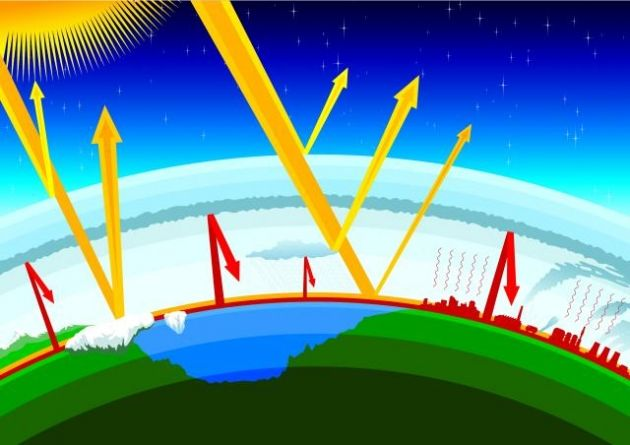
\includegraphics[width=0.5	\textwidth]{./Figures/cap2/calentamientoGlobal.jpg}
    	\caption{Calentamiento Global \cite{calent2015global}.}
    	\label{fig:cambioClimatico}
    \end{figure}


\section{Ciclo de carbono} 
Las plantas absorben el dióxido de carbono existente en el aire o el agua, acumul\'andolos en los tejidos vegetales en forma de materia org\'anica, mediante la fotos\'intesis \cite{natur2015PW}. Posteriormente, los animales herb\'ivoros se alimentan de estos vegetales para transferir esa energ\'ia a los dem\'as niveles (carnívoros que se alimentan de los herb\'ivoros).
La energía transferida sigue varios caminos: por un lado es devuelto a la atm\'osfera como di\'oxido de carbono mediante la respiraci\'on; por otro lado se deriva hacia el medio acu\'atico, donde puede quedar como sedimentos org\'anicos, o combinarse con las aguas para producir carbonatos y bicarbonatos (suponen el 71\% de los recursos de carbono de la Tierra). La acumulaci\'on de carbono en zonas h\'umedas genera turba (Carb\'on ligero y esponjoso), resultado de una descomposición incompleta, lo que da lugar a la formaci\'on de dep\'ositos de combustibles f\'osiles como petr\'oleo, carb\'on y gas natural.\\~\\
El ciclo del carbono queda completado gracias a los organismos des\-componedores, los cuales llevan a cabo el proceso de mineralizar y descomponer los restos org\'anicos, cad\'averes, excrementos, entre otros. Adem\'as de la actividad que llevan a cabo el reino vegetal y animal en el ciclo, tambi\'en liberan carbono la putrefacci\'on y la combusti\'on \cite{natur2015PW}. La figura \ref{fig:ciclocarbono} nos presenta el ciclo completo del carbono.
    \begin{figure}[!hbtp]
    	\centering
    	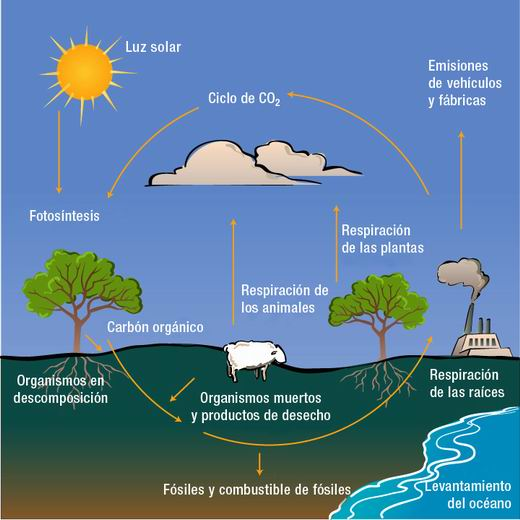
\includegraphics[width=0.5	\textwidth]{./Figures/cicloCarbono.jpg}
    	\caption{Ciclo de carbono \cite{ciclot2015carbo}.}
    	\label{fig:ciclocarbono}
    \end{figure}


\subsection{Secuestro de carbono}
El CO2 y otros gases invernaderos actúan atrapando la energ\'ia cal\'orica (radiación solar de onda corta) reflejada de la superficie de la tierra y las nubes \cite{encaptura}. Este calor retenido puede conducir al calentamiento global en el planeta. Los niveles del di\'oxido de carbono atmosf\'erico pueden reducirse en la misma medida que los niveles de carbono org\'anico del suelo aumentan a trav\'es del secuestro de carbono. Si el carbono org\'anico del suelo no es alterado, puede permanecer en el suelo por muchos a\~{n}os como materia org\'anica estable. Este carbono es entonces secuestrado o removido de la atm\'osfera para ser reciclado. De esta forma se pueden reducir los niveles de CO2, disminuyendo las probabilidades de calentamiento global \cite{castillo2003manejo}.
\subsection{P\'erdida de Carbono}
P\'erdida de carbono se refiere a aquella porci\'on de carbono que no pudo ser almacenada o capturada en el intercambio normal que ocurre entre la superficie terrestre y la atm\'osfera en el ciclo de carbono \cite{marquezestimacion}, contribuyendo al calentamiento global mediante la emisión de di\'oxido de carbono que compone el grupo de gases de efectos invernaderos.
\subsection{Secuestro de carbono en Paraguay}
El Fondo para el Medio Ambiente Mundial (FMAM) y el Programa de Peque\~{n}as Donaciones (PDD), en nuestro pa\'is, nos dice que el uso de hidrocarburos para generar energ\'ia el\'ectrica, el uso de biomasa como fuente de energ\'ia, las emisiones industriales, la deforestaci\'on, los incendios forestal, la actividad pecuaria, el manejo y disposici\'on de residuos y la actividad del transporte son los que presentan mayores emisiones de carbono \cite{cecilia2010Proyecto}, en consecuencia contribuyen al cambio clim\'atico.
\subsection{Gran Chaco Americano}
En el territorio del Gran Chaco Americano, se detecta una tendencia de importante aumento de las tasas de deforestaci\'on diaria por encima de las 1.400 hect\'areas, siendo el promedio del per\'iodo 15 de junio al 10 de julio de 2.011, de 1.042 hect\'areas por d\'ia, y del per\'iodo 10 de julio al 13 de agosto de 2.011 de 1.408 hect\'areas por d\'ia en toda la regi\'on, dando un total de 47.856 hect\'areas de \'areas boscosas que registraron cambio a uso agropecuario, en 34 d\'ias. Entre los pa\'ises que componen el Gran Chaco Americano,  Paraguay  registr\'o el mayor porcentaje de la deforestaci\'on (86\%), seguido por Argentina (13\%) y Bolivia (1\%). En Brasil, no se detectaron caso de deforestaci\'on para la regi\'on. En el caso espec\'ifico de Paraguay, la tasa de deforestaci\'on diaria ha aumentado, pasando de 998 hect\'areas por d\'ia a 1.210 hect\'areas por d\'ia \cite{fao2003revista}, perdi\'endose por consiguiente en gran medida sumideros de carbono, lo cual va aportando al desequilibrio del ciclo. En la tabla \ref{tab:chacoamericano} podemos observar los principales problemas ambientales que afronta el Gran Chaco Americano, en cada pa\'is que lo compone.
\begin{table}[!hbtp]
	\centering
	\caption{Problem\'atica que afrontan los países del gran chaco americano \cite{gustavo2012deteccion}.}
	\label{tab:chacoamericano}
	\begin{tabular}{|p{4cm}|p{4cm}|p{4cm}|}
		\hline
		{\bf Argentina} & {\bf Bolivia} & {\bf Paraguay} \\ \hline
		Deforestaci\'on de los bosques nativos. & Deforestaci\'on de los bosques nativos. & Deforestaci\'on de los bosques nativos. \\ \hline
		Excesiva dependencia dela producci\'on ganadera y explotaci\'on forestal. & Sobrepastoreo. & Sobrepastoreo. \\ \hline
		Sobrepastoreo. & Incendios de bosques y pastizales. & Incendios de bosques y pastizales. \\ \hline
		Incendios de bosques y pastizales. & P\'erdida de biodiversidad. & Manejo no sustentable de los recursos h\'idricos. \\ \hline
		Perdida de labiodiversidad. & Cambio clim\'atico. & P\'erdida de biodiversidad. \\ \hline
		Cambio clim\'atico. &  & Cambio clim\'atico. \\ \hline
	\end{tabular}
\end{table}


\section{Biomasa}
La biomasa es aquel material org\'anico biodegradable y no fosilizado originado de plantas, animales y microorganismos; incluye productos, subproductos, residuos y desechos de la agricultura, forester\'ia e industrias afines, as\'i como las fracciones org\'anicas y no fosilizadas de los desechos industriales y municipales. La biomasa tambi\'en incluye los gases y l\'iquidos recuperados de la descomposici\'on de materiales org\'anicos biodegradables y no fosilizados \cite{salinas2008guia}.
La biomasa es considerada como la masa total de organismos vivos en una zona o volumen determinado (a menudo también se incluyen los restos de plan que han muerto recientemente). La cantidad de biomasa se expresa mediante su peso en seco o su contenido de energ\'ia de carbono o de nitr\'ogeno \cite{garciduenas1987produccion}.
\subsection{Biomasa Forestal}
La biomasa forestal se define como el peso (o estimaci\'on equivalente) de materia org\'anica que
se encuentra en un determinado ecosistema forestal por encima y por debajo del suelo \cite{schlegel2000manual}, normalmente es
cuantificada en toneladas por hect\'area de peso verde o seco. La biomasa forestal es frecuentemente separada en
componentes, donde los m\'as t\'ipicos corresponden a la masa del fuste, ramas, hojas, corteza,
ra\'ices, hojarasca y madera muerta. \\~\\
En t\'erminos de p\'erdida y secuestro, representa la cantidad potencial de carbono que puede ser liberada a la atm\'osfera, debida a la deforestaci\'on, o la conservada en superficies terrestres cuando los bosques son correctamente gestionados \cite{lu2005exploring}.

\section{Medici\'on de balances de carbono}
La din\'amica del balance de carbono en un ecosistema forestal es muy compleja de medir, ya que es necesario determinar la captura de carbono por crecimiento de biomasa en los \'arboles y otros componentes en la vegetaci\'on como las p\'erdidas ocasionadas por disturbios, sean naturales o por actividades humanas; descomposici\'on de madera muerta; y la transferencia entre los compartimentos vivos, muertos y el suelo \cite{angelsen2008moving}.\\~\\
Existen metodolog\'ias que permiten medir y monitorear cambios en reservorios promedios de carbono por unidad de \'area. A continuaci\'on podemos citar algunos de ellos:

\begin{itemize}
	
	\item \textbf{Inventarios forestales:} se establecen relaciones alom\'etricas con mediciones de terreno en funci\'on al di\'ametro o volumen de arboles con las reservas de carbono forestal. La desventaja que presenta es su lentitud al realizar en \'areas grandes y costo elevado que presenta \cite{asner2005selective}. Definiendo alom\'etria como los cambios de dimensi\'on relativa de las partes corporales correlacionados con los cambios en el tama\~{n}o total. 
	\item \textbf{Sensores remotos:} existen diferentes tipos de sensores que permiten monitorear cambios en reservorios de carbono vegetal con mayor dinamismo y a gran escala \cite{libro2012Tsuyuki}:
	\begin{enumerate}
	\item \textbf{Sensores remotos \'opticos (pasivos):} capturan luz solar o artificial reflejada desde el objeto, detectando la intensidad de luz visible e infrarroja en una o mas longitudes de ondas.
	\item  \textbf{Sensores remotos activos:} este sensor se encuentra montado en un sat\'elite, el cual emite pulsos de microondas oblicuamente detectando y registrando la intensidad, fase y tiempo de los impulsos reflejados desde la superficie terrestre.
	\item  \textbf{Sensores remotos l\'aser como LiDAR (detecci\'on \'area de luz y medidas de rango):} mide la distancia entre el sensor y el objeto usando el tiempo que tarda el pulso en viajar y la intensidad del pulso reflejado del objeto.
	\end{enumerate}
	La figura \ref{fig:sensores} nos muestra como la informaci\'on es capturada, por medio de los 3 tipos de sensores descriptos.  
	    \begin{figure}[!hbtp]
	    	\centering
	    	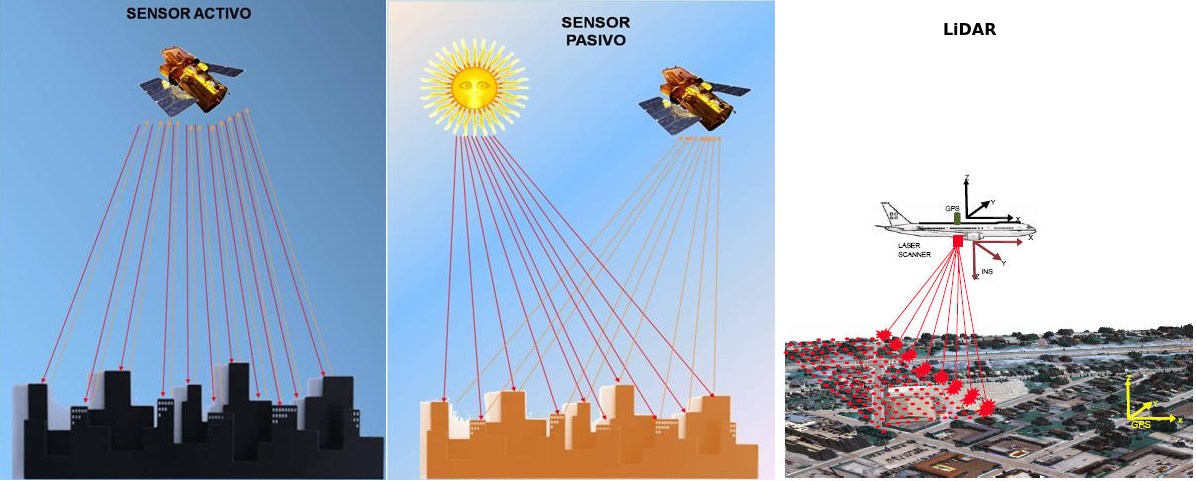
\includegraphics[width=0.9	\textwidth]{./Figures/sensores.png}
	    	\caption{Tipos de sensores.}
	    	\label{fig:sensores}
	    \end{figure}
\end{itemize}

\section{Teledetecci\'on en el medio ambiente}
El t\'ermino teledetecci\'on esta definida como la ciencia y arte de obtener informaci\'on referente a la superficie terrestre sin entrar en contacto con ella. Esto se realiza detectando y grabando la energ\'ia emitida o reflejada para su procesamiento, an\'alisis y aplicaci\'on de esa informaci\'on \cite{salinero2002teledeteccion}.\\~\\
En los \'ultimos a\~{n}os se han desarrollado bastantes aplicaciones en casi todas las \'areas que involucra la tierra, debido a las grandes posibilidades y ventajas que presenta con la localizaci\'on de espacios geogr\'aficos, observaci\'on de fen\'omenos temporales e integraci\'on de resultados a los sistemas de informaci\'on geogr\'afica, reduciendo los costos en dinero y tiempo empleados en estudios sobre el terreno \cite{baker2006mapping}. La aplicaci\'on de la teledetecci\'on en los recursos naturales se fundamenta en que los elementos del mismo tienen un respuesta espectral propia a los sensores remotos. Por ello, la teledetecci\'on espacial es empleada como complemento y no como sustituto a estudios ambientales por permitir realizarlos a escalas espaciales y temporales distintas a las que se acceden desde experimentos controlados, lo cuales son tambi\'en necesarios e imprescindibles pero a veces insuficientes \cite{perez2011aplicaciones}.\\~\\
En la figura \ref{fig:tele}, podemos observar todo el proceso que implica el uso de la teledetecci\'on.

	\begin{figure}[H]
		\centering
		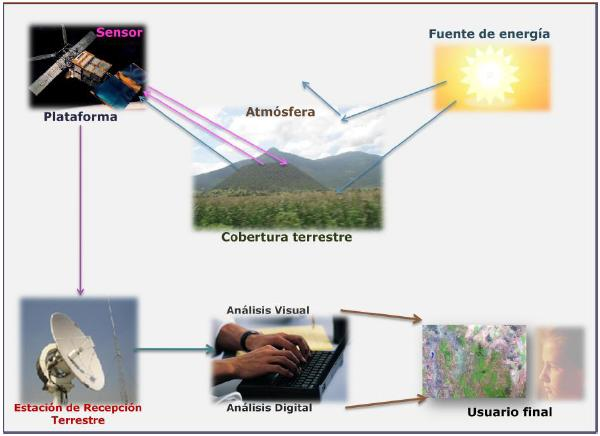
\includegraphics[width=0.7	\textwidth]{./Figures/cap3/teledeteccion.png}
		\caption{Teledetecci\'on \cite{teledet2015perce}.}
		\label{fig:tele}
	\end{figure}

\section{Resumen}

La perdida de los bosques provocan da\~{n}os con consecuencias exponenciales al medio ambiente, ya que representan un factor fundamental en la estabilidad clim\'atica de la tierra. Las tierra esta cubierta por gases que dejan penetrar la energ\'ia solar, manteniendo temperaturas optimas para la vida. Algunos de los gases impiden el escape del calor hacia el espacio, a estos gases se los llaman gases de Efecto Invernadero (GEI). Las actividades humanas producen en exceso los GEI, principalmente con di\'oxido de carbono (CO2) a trav\'es de la deforestaci\'on y degradaci\'on en los bosques. La fotos\'intesis compone un elemento fundamental en el proceso natural denominado ciclo del carbono, mitigando el CO2 de la atm\'osfera con transformaciones del gas a materia org\'anica en las plantas (biomasa), a esto se lo conoce como secuestro de carbono. El chaco paraguayo presenta una tendencia importante en el aumento de las tasas de deforestaci\'on, siendo entre los pa\'ises que componen el Gran chaco americano el que presenta mayor porcentaje (86\%). 
En el 2011, el chaco paraguayo registro un promedio diario de 1402 hect\'areas de bosques deforestados a causa de actividades humanas ligadas a la agricultura, silvicultura y ganadería, por ello la medici\'on del balance de carbono en nuestro pa\'is resulta importante para controles del manejo del medio ambiente. Los inventarios forestales establecen relaciones entre reservas de carbono forestal y variables alom\'etricas de los arboles  para medir el contenido de carbono, presentando como principal dificultad la lentitud en el estudio de \'areas extensas. En cambio, el empleo de procesamiento digital de im\'agenes satelitales junto con la teledetecci\'on nos brindan un dinamismo en el monitoreo a gran escala.

\newpage{\ } 
\thispagestyle{empty} 

\chapter{Procesamiento de im\'agenes satelitales}
\lhead{Capítulo 3. \emph{Procesamiento de im\'agenes satelitales}} % This is for the header on each page - perhaps a shortened title
La teledetecci\'on presenta un principio base similar al de la visi\'on, permitiendo mediante una fuente de energ\'ia, un objetivo o escena y un sensor, generar im\'agenes digitales que posibilitan resaltar aquellos elementos dif\'iciles de percibir o ser distinguidos directamente a trav\'es de una imagen normal. A todo esto sum\'andole el comportamiento caracter\'istico que poseen los recursos naturales a sensores espaciales, nos posibilita el empleo amplio de t\'ecnicas de procesamiento de im\'agenes provechosos para el logro de los objetivos en la investigaci\'on. Este capitulo consiste en brindar conceptos espec\'ificos utilizados por la metodolog\'ia, posibilitando comprender la influencia de cada factor en el empleo de im\'agenes satelitales para la estimaci\'on de p\'erdida del contenido de carbono forestal.

\section{Sensores Remotos}
Los sensores remotos nos permiten obtener informaci\'on de la superficie terrestre, soportados en diferentes plataformas (terrestre, \'area y satelital), mediante la captura de energ\'ias reflejadas o radiadas proveniente del sol (sensores pasivos) o del mismo sensor (sensores activos) para luego ser transformadas en productos con diversos y diferentes especificaciones, siendo fotografi\'as \'areas e im\'agenes de sat\'elites los m\'as conocidos.
\subsection{El espectro electromagn\'etico}
A pesar de que las longitudes de ondas son continuas, se establece un serie de bandas donde las radiaciones manifiestan un comportamiento similar organizando las de este modo, en un espectro electromagn\'etico\cite{remote2010abdulrahman}.
Las bandas m\'as empleadas son las siguientes\cite{salinero2002teledeteccion}:
	\begin{itemize}
		\item \textbf{Espectro visible:} (400 nm a 700 nm) se denomina as\'i por tratarse de la \'unica radiaci\'on electromagn\'etica que pueden percibir nuestros ojos, coincidiendo con las longitudes de onda en donde es m\'axima la radiaci\'on solar. Dentro de esta se distinguen tres bandas fundamentales: Azul (400 nm a 500 nm), verde (500 nm a 600 nm) y rojo (600 nm a 700 nm).
		\item \textbf{Infrarrojo pr\'oximo:} (700 nm a 1300 nm) se utiliza para discriminar masas vegetales y concentraciones de humedad.
		\item \textbf{Infrarrojo medio:} (1,3 um a 8 um) en esta franja se entremezclan los procesos de reflexi\'on de la luz solar y de emisi\'on de la superficie terrestre. Se utiliza para estimar contenido de humedad en la vegetaci\'on y los focos de alta temperatura.
		\item \textbf{Infrarrojo lejano o térmico:} (8 um a 14 um) se detecta el calor de la mayor\'ia de las cubiertas terrestres.
		\item \textbf{Microondas:} (a partir de 1 um) de gran inter\'es por ser un tipo de energ\'ia transparente a la cubierta nubosa.
	\end{itemize}
	\begin{figure}[H]
		\centering
		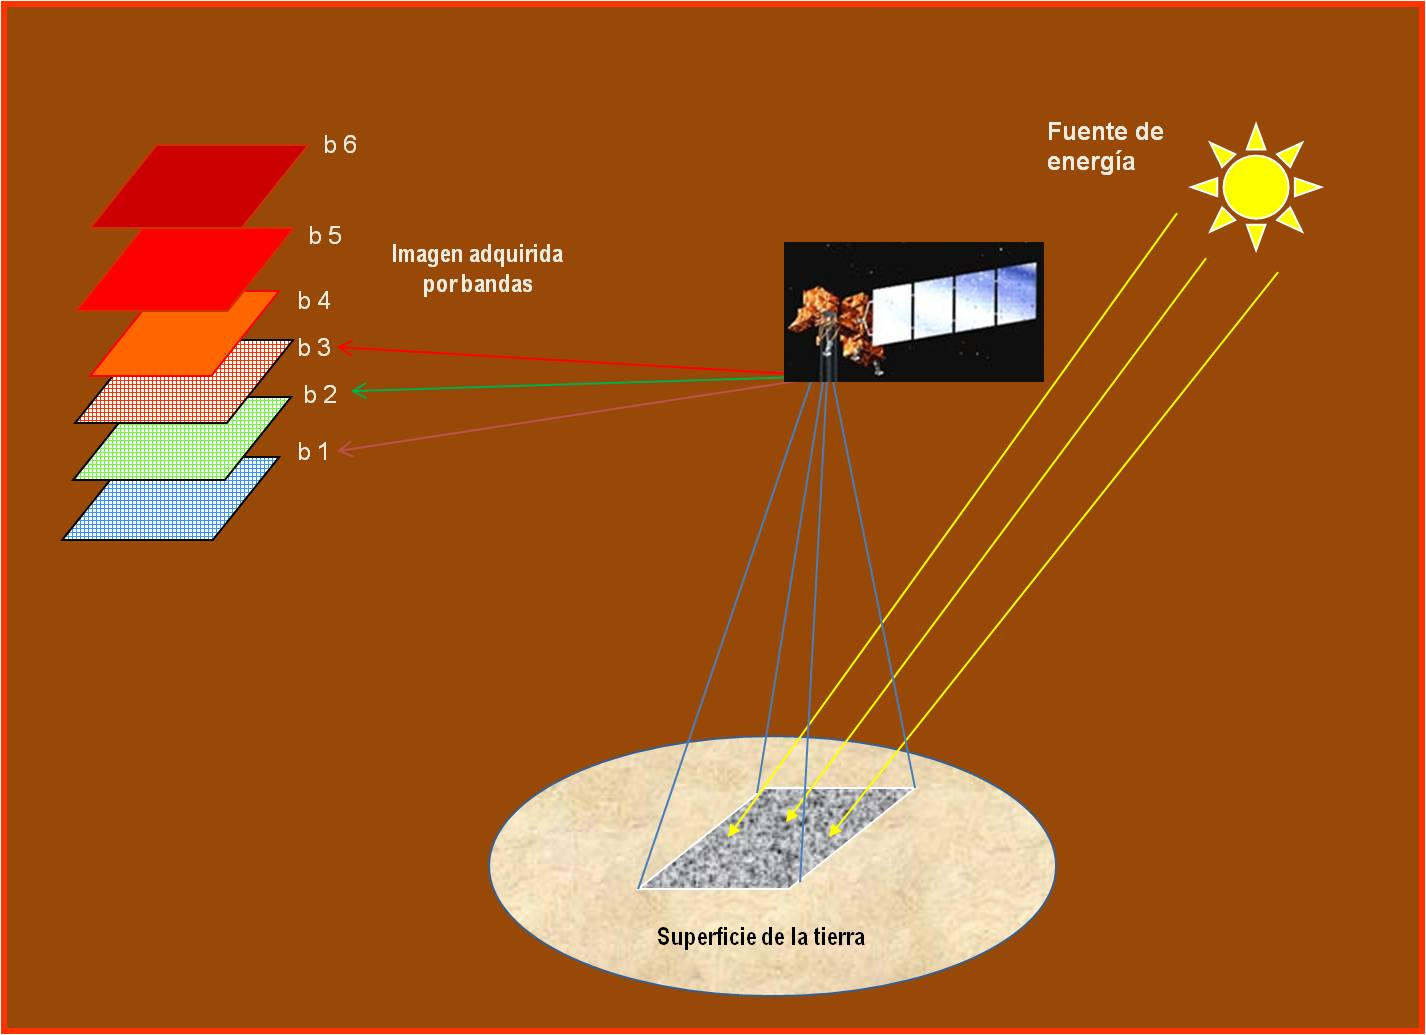
\includegraphics[width=0.7	\textwidth]{./Figures/cap3/bandas_imagen.png}
		\caption{Bandas capturadas por un sat\'elite.}
		\label{fig:bandasIs}
	\end{figure}

\subsection{Firmas espectrales}
Las firmas espectrales consisten en la representaci\'on de energ\'ia reflejada con relaci\'on a las longitudes de ondas, consideradas sin el efecto atmosf\'erico y medida en condiciones ideales del \'angulo incidente. Ayudan a identificar los objetos en la superficie terrestre debido a que cada uno presenta una respuesta espectral \'unica\cite{sivakumar2004satellite}.\\~\\
En la siguiente figura se observa como cada objeto difiere de los dem\'as en sus firmas espectrales:

\begin{figure}[H]
	\centering
	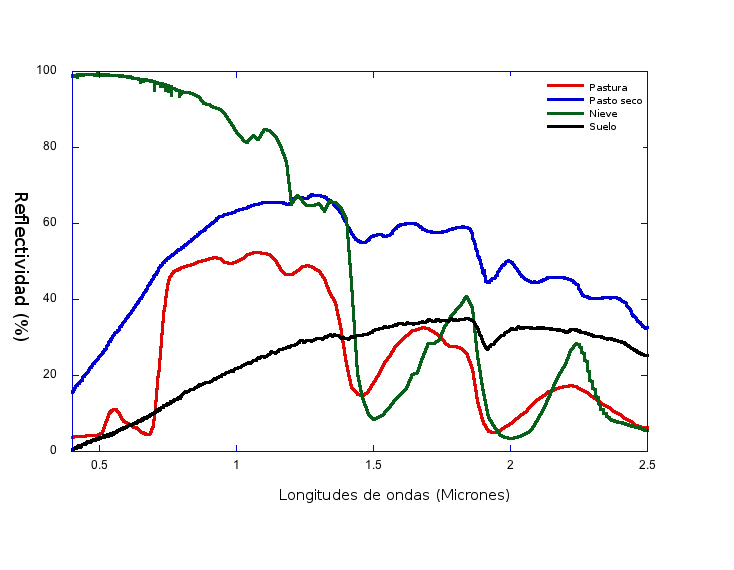
\includegraphics[width=0.9	\textwidth]{./Figures/cap3/firmaEspectral.jpg}
	\caption{Firmas espectrales de diferentes coberturas.}
	\label{fig:firmaEspectral}
\end{figure}

\subsection{Resoluciones de un sensor}

Se define a la resoluci\'on de un sensor como el menor cambio en la magnitud de entrada que puede ser apreciada en la magnitud de salida. El concepto de resoluci\'on implica al menos cuatro manifestaciones \cite{peralta2013analisis}: 
	\begin{itemize}
		
		\item \textbf{Resolución espacial:} Es el tamaño que representa en el terreno una unidad de pixel de la imagen. Tiene mucha importancia en la interpretaci\'on pues marca el nivel de detalle que ofrece, cuanto menor sea el tama\~{n}o del pixel, menor ser\'a tambi\'en la probabilidad de que corresponda a un compuesto de dos o m\'as \'areas fronterizas.
		\begin{figure}[H]
			\centering
			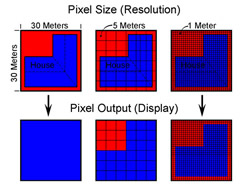
\includegraphics[width=0.4	\textwidth]{./Figures/cap3/espatialRes.jpg}
			\caption{Resoluci\'on espacial.}
			\label{fig:espatialRes}
		\end{figure}
			\item \textbf{Resoluci\'on espectral:} Indica el n\'umero y anchura de las bandas espectrales que puede discriminar el sensor. Un sensor ser\'a tanto m\'as id\'oneo cuanto mayor n\'umero de bandas proporcione, ya que facilita la caracterizaci\'on espectral de las distintas cubiertas.
				\begin{figure}[H]
					\centering
					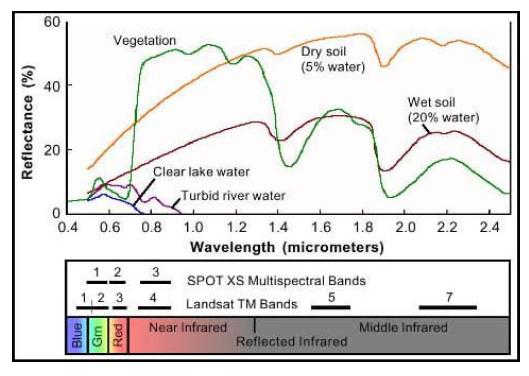
\includegraphics[width=0.6	\textwidth]{./Figures/cap3/resolucionespectral.jpg}
					\caption{Resoluci\'on espectral igual a 3 para el sensor SPOT y 7 en el sensor Landsat.}
					\label{fig:espectralRes}
				\end{figure}
		\item \textbf{Resoluci\'on radiom\'etrica:} Es la sensibilidad del sensor para detectar variaciones en la cantidad de energ\'ia espectral recibida. La sensibilidad se expresa en bits e indica el n\'umero de los distintos niveles radiom\'etricos $ r $ que puede detectar un sensor.
		\nomenclature[10]{$ r $}{Bits o Niveles radiom\'etricos de la imagen satelital.}	
						\begin{figure}[H]
							\centering
							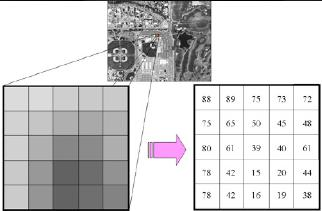
\includegraphics[width=0.6	\textwidth]{./Figures/cap3/resolucionradiometrica.jpg}
							\caption{Resoluci\'on radiom\'etrica de 8 bits (0 a 255 niveles digitales).}
							\label{fig:radioRes}
						\end{figure}
		\item \textbf{Resoluci\'on temporal:} Este tipo de resoluci\'on se refiere al intervalo de tiempo entre muestras sucesivas de la misma zona de la cobertura terrestre. El ciclo de cobertura est\'a en funció\'on de las caracter\'isticas orbitales de la plataforma, su velocidad, el ancho de barrido del sensor y las caracter\'isticas de construcci\'on del sistema.
			\begin{figure}[H]
					\centering
					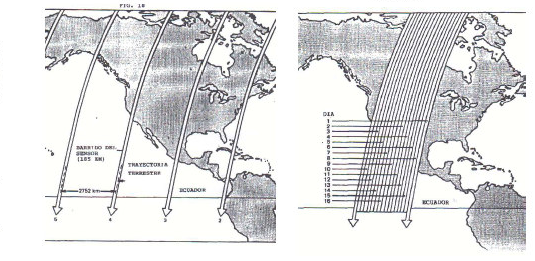
\includegraphics[width=0.6	\textwidth]{./Figures/cap3/resolucion_temporal_land.png}
					\caption{Resoluci\'on temporal de 16 d\'ias.}
					\label{fig:temporaRes}
				\end{figure}
		

		
	\end{itemize}

\section{Im\'agenes satelitales}
%Una imagen satelital o imagen de sat\'elite $ S $ se puede definir como la representaci\'on visual de la informaci\'on capturada por un sensor montado en un sat\'elite artificial. Est\'an organizados en un arreglo matricial bidimensional $ l \times c $ de elementos llamados p\'ixeles, donde cada p\'ixel representa un \'area de superficie sobre la tierra con un valor de intensidad o nivel digital $ f(x,y) $, dentro del dominio $ D=[0,2^{r}] $, y una ubicación en la imagen  $(x,y)$, tambi\'en son conocidas como im\'agenes r\'aster \cite{acosta2003experiencia}. 
%		\nomenclature[11]{$ S $}{Imagen satelital.}	
%\begin{equation}
%\label{eq:imagenDigital}
%f(x,y)=\begin{bmatrix}
%f(0,0) &f(0,1)  & \cdots & f(0,c-1) \\ 
%f(1,0) & f(1,1) & \cdots  & f(1,c-1)\\ 
%\vdots & \vdots & & \vdots \\ 
%f(l-1,0) & f(l-1,1)  &\cdots  & f(l-1,c-1)
%\end{bmatrix}
%\end{equation}
Una imagen satelital se puede definir como la representaci\'on visual de la informaci\'on capturada por un sensor montado en un sat\'elite artificial \cite{acosta2003experiencia}. \\~\\
Sea $ \mathbb{Z} $ un conjunto de enteros. Una imagen satelital es una funci\'on $ f:\mathbb{Z}^{3} \longrightarrow \{0,...,2^{r}\} $. Cada $ (x,y,i) $ se los conoce como coordenadas espaciales de la banda $ i $, donde $ i \in \{1,...,k\} $, $ x \in \{0,...,m\} $ e $ y \in \{0,...,n\} $ para una matriz $ m \times n $, siendo $ k $ el numero de bandas y $ r $ la resoluci\'on radiom\'etrica en la imagen. Las im\'agenes satelitales son conocidos tambi\'en como raster.
  \begin{figure}[H]
  	\centering
  	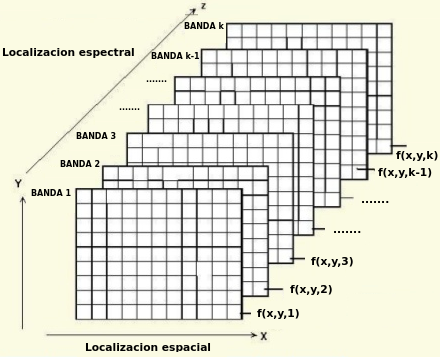
\includegraphics[width=0.8	\textwidth]{./Figures/cap3/imagen_satelital.png}
  	\caption{Imagen satelital.}
  	\label{fig:imagenMultiespectral}
  \end{figure}
  	\nomenclature[11]{$\mathbb{Z}$}{Conjunto de enteros.}
  	\nomenclature[12]{$i$}{ Banda de la imagen satelital.}
  	\nomenclature[13]{$f$}{ Imagen satelital.}
  	\nomenclature[13]{$(x,y)$}{ Coordenadas espaciales.}
  	\nomenclature[16]{$(x,y,i)$}{Coordenadas espaciales de la banda $ i $ en la imagen satelital.}
  	\nomenclature[17]{$k$}{ N\'umero de bandas que posee una imagen satelital.}
  	\nomenclature[18]{$f(x,y,i)$}{ Nivel digital, en la posici\'on $ (x,y) $ de la banda $ i $, de la imagen satelital.}
La ilustraci\'on \ref{fig:imagenMultiespectral} nos muestra los ejes de coordenadas espaciales $ (x,y) $ para cada plano que representan las bandas, pudiendo acceder a valor de la intensidad o nivel digital mediante la funci\'on $ f(x,y,i) $.


\subsection{Histogramas}
El histograma es una representaci\'on gr\'afica \'util de la informaci\'on contenida por las im\'agenes obtenidas a trav\'es de la percepci\'on remota. Los analistas, a menudo despliegan el histograma ya que proporciona una apreciaci\'on de la calidad de los datos que presenta una imagen. Por ejemplo si el contraste es bajo o muy alto (histogramas estrechos y amplios); si son multimodales responden a distintos tipos de coberturas detectadas (agua, humedales, tipos de vegetaci\'on, etc.), si el histograma se encuentra desplazado hacia la izquierda, la imagen tendr\'a una tonalidad oscura y si esta desplazada hacia la derecha tendr\'a una tonalidad mas clara; entre otras interpretaciones.

\subsection{Combinaci\'on de bandas}
Las im\'agenes satelitales suelen ser multiespectrales, es decir que son registradas simult\'aneamente en varias regiones del espectro electromagn\'etico (Bandas). Estas im\'agenes pueden ser estudiadas individualmente en escalas de grises o en im\'agenes coloreadas obtenidas a partir de las primeras. Las im\'agenes coloreadas se generan seg\'un el modelo de color RGB ( Red, Green, Blue). Este hace referencia a la composici\'on del color en t\'erminos de la intensidad de los colores primarios con los que se forma: el rojo, el verde y el azul. Es un modelo de color basado en la s\'intesis aditiva, es decir basado en la mezcla por adici\'on de dichos primarios\cite{teledet2015Combi}.
Mediante el estudio en cada banda, y la combinaci\'on de ellas, es posible resaltar variaciones de color, tonalidad, textura de las rocas, etc. A continuaci\'on se describe algunas combinaciones posibles con im\'agenes Landsat para la identificacion visual de aspectos terrestres\cite{lillesand2014remote}:
	\begin{itemize}
		\item \textbf{Bandas 3,2,1 (RGB):} Es una imagen de color natural. Refleja el \'area tal como la observa el ojo humano en una fotograf\'ia a\'erea a color.
		\item  \textbf{Bandas 7,4,2 (RGB):} Permite discriminar los tipos de rocas. Ayuda en la interpretaci\'on estructural de los complejos intrusivos asociados a los patrones volcano - tect\'onicos.
		\item  \textbf{Bandas 5,4,2 (RGB):} Es una imagen que no refleja los patrones en colores naturales (falso color), por lo tanto las carreteras pueden ser rojas, el agua amarilla y la vegetaci\'on azul.
		\item \textbf{Bandas 7,3,1 (RGB):} Ayuda a diferenciar tipos de rocas, definir anomal\'ias de color que generalmente son de color amarillo claro algo verdoso, la vegetaci\'on es verde oscuro a negro, los r\'ios son negros y con algunas coloraciones azules a celestes.		
	\end{itemize}
 
  \begin{figure}[H]
  	\centering
  	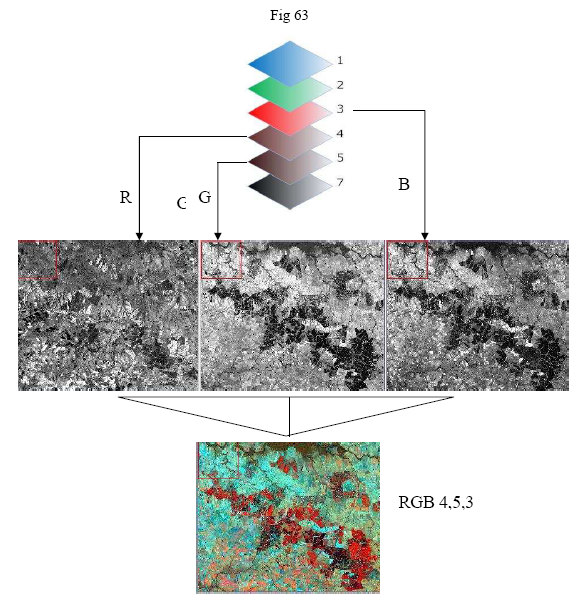
\includegraphics[width=0.8	\textwidth]{./Figures/cap3/combinacionColor.jpg}
  	\caption{Combinaci\'on de bandas espectrales a trav\'es de los canales RGB.}
  	\label{fig:combinacionColor}
  \end{figure}

 
\section{\'Indices de vegetaci\'on}
Los \'indices de vegetaci\'on son transformaciones que implican efectuar una combinaci\'on matem\'atica, entre los niveles digitales almacenados en dos o m\'as bandas espectrales de la misma imagen, teniendo en cuenta el comportamiento radiom\'etrico de la vegetaci\'on vigorosa para la elecci\'on de bandas\cite{speranza2005potencialidad}. \\~\\
El estudio de las cubiertas vegetales mediante la teledetecci\'on se aborda tradicionalmente mediante la utilización de los denominados “índices de vegetaci\'on”, siendo el m\'as utilizado el \'Indice de vegetaci\'on diferencial normalizada (NDVI) \cite{sader2000estimacion}.

\subsection{\'Indice de vegetaci\'on diferencial normalizada}\label{subsec:ndvi}
El NDVI es un \'indice usado para estimar la cantidad, calidad y desarrollo de la vegetaci\'on por medio de sensores remotos instalados com\'unmente desde la plataforma espaciales, es decir mide las condiciones de vigor vegetal de la planta, principalmente su contenido en clorofila \cite{salinero2002teledeteccion}. El objetivo del NDVI es la reducci\'on de m\'ultiples bandas a una sola, condensando la informaci\'on m\'as importante, en este caso la vegetaci\'on.\\~\\
Chuvieco \cite{salinero2002teledeteccion} menciona que la principal ventaja del NDVI es su f\'acil interpretaci\'on, ya que sus
valores var\'ian entre -1 y +1, permitiendo conocer el estado de vigor vegetal en grandes superficies y detecta fen\'omenos de amplio rango.\\~\\
Sea $ ndvi:(x,y) \longrightarrow [-1,1] $ una funci\'on que determina la imagen con los NDVI en cada coordenada espacial, $ R \in \{1,...,k\}$ representa la banda roja del espectro visible y $ IRc \in \{1,...,k\}$ la banda infrarroja cercana del espectro infrarrojo, queda definida la siguiente expresi\'on:
	\begin{equation}
	\label{e:ndvi}
	ndvi(x,y)=\dfrac{f(x,y,IRc)-f(x,y,R)}{f(x,y,IRc)+f(x,y,R)}
	\end{equation}
	\nomenclature[19]{$ndvi$}{Imagen del \'indice de vegetaci\'on diferencial normalizada (NDVI).}
	\nomenclature[20]{$ndvi(x,y)$}{ NDVI de las coordenadas $ (x,y) $.}
	\nomenclature[21]{$R$}{ Posici\'on de la banda Roja en la imagen satelital.}
	\nomenclature[22]{$IRc$}{ Posici\'on de la banda Infrarroja cercana en la imagen satelital.}
Las plantas muestran un fuerte pico de absorci\'on causados por los pigmentos fotosint\'eticos en longitudes de onda cercanas a los 700 micrones, hecho que contrasta con una fuerte reflexi\'on de las longitudes de onda del infrarrojo cercano \cite{salinero2002teledeteccion}. Por su parte, los suelos desnudos se caracterizan por un incremento suavemente monot\'onico de la reflectancia, a medida que aumenta la longitud de onda \cite{salinero2002teledeteccion}.

\section{An\'alisis Multitemporal}
B\'asicamente el an\'alisis multitemporal consiste en el estudio de zonas determinadas mediante tomas hechas en diferentes tiempos, Chuvieco \cite{salinero2002teledeteccion} resalta que el factor temporal puede abordarse con un doble objetivo: por un lado reconstruir la variaci\'on estacional de la zona y por otra parte la detecci\'on de cambios, esta \'ultima se enfoca a detectar cambios entre dos o m\'as
fechas alejadas en el tiempo, estudia el dinamismo temporal de una determinada zona, como por ejemplo: el crecimiento urbano, transformaciones agrícolas, entre otras.\\~\\
Sea uno u otro el enfoque aplicado al estudio multitemporal, resulta preciso abordar previamente una serie de tratamientos sobre las im\'agenes satelitales de cara a garantizar su comparabilidad, ya que existen factores, naturales o las del sensor, que influye desde la captura de informaci\'on hasta su transformaci\'on final a niveles digitales que podr\'ian afectar el an\'alisis.


\section{Correciones a las im\'agenes de sat\'elites}
Una imagen de sat\'elite est\'a sometida a una serie de interferencias que hacen que la informaci\'on que quiere obtenerse aparezca perturbada por una serie de errores:
	\begin{itemize}
		\item Fallos en los sensores, generan pixeles incorrectos.
		\item Alteraciones en el movimiento del sat\'elite y el mecanismo de captaci\'on e los sensores, generan
		distorsiones en la imagen global.
		\item Interferencia de la atm\'osfera, alteran de forma sistem\'atica los valores de los pixeles.
	\end{itemize}


\subsection{Correccci\'on geom\'etrica}\label{sec:corrGeometrica}
Una imagen de sat\'elite, al igual que las fotograf\'ias a\'ereas, no proporciona informaci\'on georreferenciada; cada pixel se ubica en un sistema de coordenadas arbitrario de tipo fila-columna como los que manejan los programas de tratamiento digital de im\'agenes.\\~\\
El proceso consiste en dar a cada pixel su localizaci\'on en un sistema de coordenadas estandard (UTM, lambert, coordenadas geogr\'aficas) para poder, de este modo, combinar la imagen de sat\'elite con otro tipo de capas en un entorno SIG. Mediante esto, se obtiene una nueva capa en la que cada columna corresponde con un valor de longitud y cada fila con un valor de latitud. En caso de que la imagen no hubiese sufrido ningún tipo de distorsi\'on, el procedimiento ser\'ia bastante sencillo, sin embargo una imagen puede sufrir diversos tipos de distorsiones.\\~\\
Es necesario localizar puntos comunes de la imagen con puntos de control, como tarea incial para la correcci\'on geom\'etrica, de manera a poder realizar una interpolaci\'on espacial y de los valores radiom\'etricos\cite{deniseCultivos}.

\subsubsection{Interpolaci\'on espacial}
Consiste en la determinaci\'on de la relaci\'on geom\'etrica entre las coordenadas del pixel de la imagen a corregir y las coordenadas correspondientes. Utilizando los puntos comunes localizados, se plantea una ecuaci\'on de transformaci\'on mediante la cual se obtiene la posici\'on de los pixeles en la imagen de salida, ilustrada en la figura \ref{fig:intEspacial}. Este proceso tambi\'en es conocido como Georreferenciaci\'on. El m\'etodo mas utilizado para la transformaci\'on es el de ecuaciones polin\'omicas. 
    \begin{figure}[H]
    	\centering
    	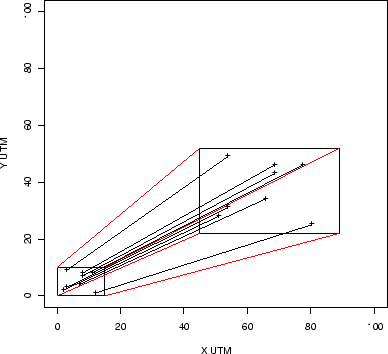
\includegraphics[width=0.9	\textwidth]{./Figures/cap3/inter_spacial.png}
    	\caption{Localizaci\'on de puntos comunes y puntos de referencia.}
    	\label{fig:intEspacial}
    \end{figure}
 
 La transformaci\'on puede expresarse de la siguiente manera:
	\begin{equation}
	x^{'}_{i} = \sum_{j=0}^{l} \sum_{d=0}^{l-j} a_{ij}x^{j}_{i}y^{d}_{i}
	\end{equation} 
		\begin{equation}
		y^{'}_{i} = \sum_{j=0}^{l} \sum_{e=0}^{l-j} b_{ij}x^{j}_{i}y^{e}_{i}
		\end{equation} 


\nomenclature[23]{$ l $}{ Grado del polinomio de ajuste.}
\nomenclature[24]{$ e $}{ Variable de iteraci\'on.}
\nomenclature[25]{$ j $}{ Variable de iteraci\'on.}

Donde $ x^{'}_{i} $ e $ y^{'}_{i} $ indica la coordenada en la imagen corregida para la banda $ i $. El superindice $ l $ indica el grado del polinomio de ajuste, $ a_{i} $ y $ b_{i} $ los coeficientes del polinomio. Siendo la ecuaci\'on lineal las mas simple:
	\begin{equation}
	x^{'}_{i} = a_{0}+a_{1}x_{i}+a_{2}y_{i}
	\end{equation} 
		\begin{equation}
		y^{'}_{i} = b_{0}+b_{1}x_{i}+b_{2}y_{i}
		\end{equation} 
		\nomenclature[26]{$ (x^{'},y^{'}) $}{Coordenadas de la imagen transformada.}
En distorsiones moderadas o en un \'area reducida, se utilizan transformaciones de primer orden, pudiendo corregir efectos de translaci\'on en $ x^{'}_{i} $ e $ y^{'}_{i} $, cambios de escala y rotaci\'on.
En distorsiones m\'as importantes o en \'areas extensas, es necesario una transfomaci\'on de segundo orden. Este tipo de transformaci\'on agregan a diferencia del primer orden, correcciones a deformaciones locales.
    \begin{figure}[H]
    	\centering
    	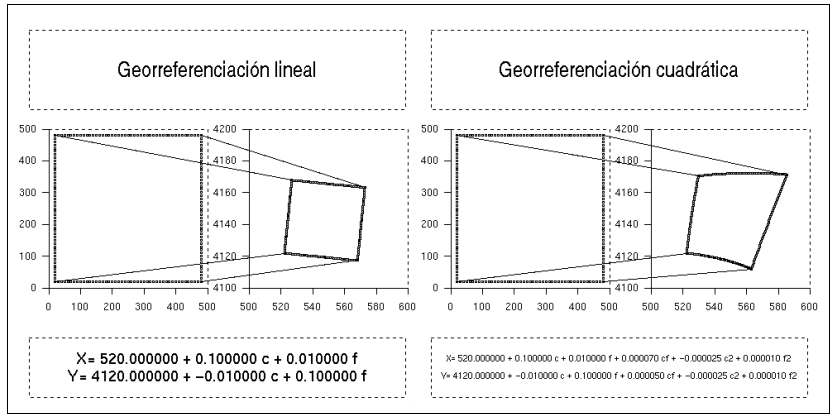
\includegraphics[width=0.9	\textwidth]{./Figures/cap3/ecuacPolinomica.png}
    	\caption{Interpolaci\'on espacial con polinomios de primer y segundo orden.}
    	\label{fig:intPolEcua}
    \end{figure}
 Para calcular la calidad en la interpolaci\'on espacial y los puntos de control seleccionados $ nc $, se utiliza el promedio de los errores cuadráticos medios (RMS), que consiste en la diferencia entre la coordenada re-transformada deseada para un punto de control y la coordenada real obtenida como salida.

 \begin{equation}
 RMS_{i} = \sqrt{\dfrac{\sum_{j=1}^{nc} ((x_{i_{j}}^{'}-x_{i_{j}})^{2}+(y_{i_{j}}^{'}-y_{i_{j}})^{2})}{nc}}
 \end{equation} 
 		\nomenclature[27]{$ RMS_{i} $}{Error cuadr\'atico de la banda $ i $.}
 		\nomenclature[28]{$ nc $}{N\'umero de puntos de control.}

 	Idealmente, el valor de RMS elegido por referencia para corregir una imagen debe ser aproximadamente $ 0.5 $, y en lo posible nunca superar la unidad \cite{guide1999erdas}.
 
 
     \begin{figure}[H]
     	\centering
     	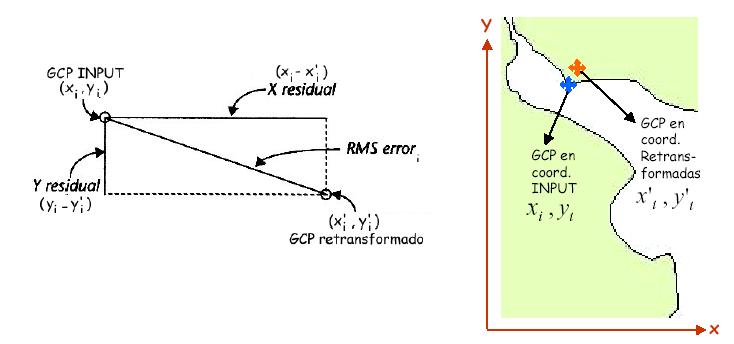
\includegraphics[width=0.9	\textwidth]{./Figures/cap4/rms.png}
     	\caption{Error RMS.}
     	\label{fig:rms}
     \end{figure}



\subsubsection{Interpolaci\'on de los valores radiom\'etricos}
La Interpolaci\'on de los valores radiom\'etricos es el traslado del nivel digital perteneciente a la imagen original, a la imagen corregida. Lo que se pretende es crear una imagen que se corresponda con estas coordenadas, por lo tanto, resulta necesario trasvasar de alguna forma, los niveles digital originales a su nueva posici\'on. Pudi\'endose ser abordada por tres m\'etodos diferentes:
	\begin{itemize}
		\item \textbf{Vecino m\'as pr\'oximo:} situ\'a en cada celda de la imagen corregida el nivel digital $ (ND) $ del pixel m\'as cercano en la imagen original. Constituye la soluci\'on m\'as r\'apida y la que supone menor transformaci\'on en los niveles digitales originales. Su principal inconveniente es que produce una distorsi\'on en rasgos lineales en la imagen(fracturas, carreteras, caminos), que pueden aparecer en la corregida como lineales quebradas. \\~\\
		Sea $ g:(x,y,i) \longrightarrow f$ una imagen interpolada radiom\'etricamente por el m\'etodo de vecino m\'as pr\'oximo en la banda $ i $:
		\nomenclature[30]{$ g $}{Imagen interpolada radiom\'etricamente por el m\'etodo de vecino m\'as pr\'oximo.}
		\nomenclature[31]{$ g(x,y,i) $}{Nivel digital en la posici\'on $ (x,y) $ de $ g $ en la banda $ i $.}
		\begin{equation}
		\Delta x = x^{'}-x
		\end{equation}	
		\begin{equation}
		\Delta y = y^{'}-y
		\end{equation}	
\begin{equation}
	g(x,y,i) = \begin{cases}
		f(x,y,i) & \text{si }\Delta x < 0.5 \text{ y } \Delta y < 0.5\\
		f(x+1,y,i) & \text{si } \Delta x \geq 0.5 \text{ y } \Delta y < 0.5\\
		f(x,y+1,i) & \text{si } \Delta x < 0.5 \text{ y } \Delta y \geq 0.5\\
		f(x+1,y+1,i) & \text{si } \Delta x \geq 0.5 \text{ y } \Delta y \geq 0.5
	\end{cases}
\end{equation}	

		En la ilustraci\'on \ref{fig:vecinoMasCercano2} se observa el procedimiento realizado.
				    \begin{figure}[H]
				    	\centering
				    	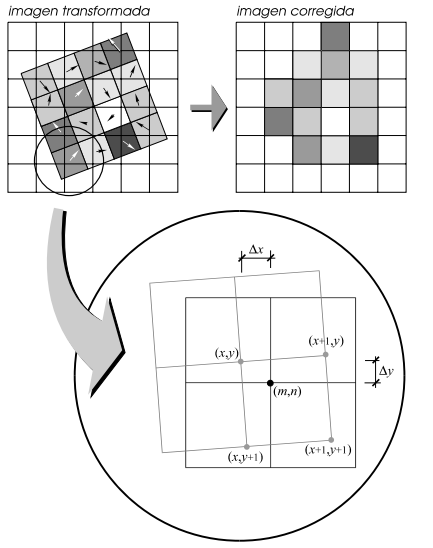
\includegraphics[width=0.6	\textwidth]{./Figures/cap3/vecinoMasCercano2.png}
				    	\caption{Interpolaci\'on Vecino m\'as Cercano.}
				    	\label{fig:vecinoMasCercano2}
				    \end{figure}
		
		\item \textbf{Interpolaci\'on bilineal:} Considera el valor de los 4 pixeles mas cercanos en la imagen de entrada para asignar el nuevo valor de la imagen de salida. Las ventajas son que no existe el efecto de escalones en los bordes pudiendo aparecer en el vecino superior izquierdo y ademas cuenta con mejor exactitud espacial. El m\'etodo es utilizado a menudo cuando se cambia el tama\~{n}o de las celdas en los datos. La desventaja es que como los pixeles son promediados, algunos extremos de los valores de los datos pueden perderse.\\~\\
		Sea $ \rho:(x,y,i) \longrightarrow f$ una imagen interpolada radiom\'etricamente por el m\'etodo bilineal en la banda $ i $:
		\begin{equation}
		\rho(x,y) = \sum_{j=1}^{4}\dfrac{(D-\Delta x_{j})(D-\Delta y_{j})}{D^{2}}f(x,y,i)
		\end{equation}	
				\nomenclature[32]{$ \rho $}{Imagen interpolada radiom\'etricamente por el m\'etodo bilineal.}
				\nomenclature[33]{$ \rho(x,y,i) $}{Nivel digital en la posici\'on $ (x,y) $ de $ \rho $ en la banda $ i $.}
		\nomenclature[33]{$ D $}{Distancia entre dos pixeles consecutivos en el eje $ x $ o $ y $ de la imagen.}
		Donde $ D $ es la distancia entre dos pixeles consecutivos en su coordenada $ x $ o $ y $ de la imagen.
		La siguiente ilustraci\'on \ref{fig:bilineal2} nos presenta gr\'aficamente el muestreo bilineal.
		    \begin{figure}[H]
		    	\centering
		    	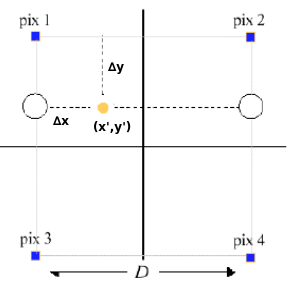
\includegraphics[width=0.7	\textwidth]{./Figures/cap3/bilineal_ecuation.png}
		    	\caption{Interpolaci\'on Bilineal.}
		    	\label{fig:bilineal2}
		    \end{figure}
		    
		    		\item \textbf{Convoluci\'on c\'ubica:} es similar a la interporlaci\'on bilineal pero considera niveles digitales de los 16 pixeles m\'as pr\'oximos. El efecto visual es m\'as correcto, pero supone un volumen de c\'alculo mucho m\'as elevado. \\~\\
					Sea $ d:(p_{x,y,i},p'_{x,y,i})\longrightarrow [0,\infty] $ la distancia euclidiana entre un pixel $ p $ con coordenadas $ (x,y,i) $ y la traslaci\'on del mismo en la imagen corregida $ (x^{'},y^{'},i)$. La funci\'on de convoluci\'on c\'ubica $ \varphi:(x,y,i) \longrightarrow f$ utilizada es la siguiente \cite{guide1999erdas}:
										\begin{align}
										\varphi(x,y,i) = \sum_{j=1}^{4} f(x-1,y+j-2,i)\beta(d(p_{x-1,y+j-2,i},p'_{x-1,y+j-2,i})+1)+ \nonumber \\
										f(x,y+j-2,i)\beta(d(p_{x,y+j-2,i},p'_{x,y+j-2,i}))+ \nonumber \\
										f(x+1,y+j-2,i)\beta(d(p_{x+1,y+j-2,i},p'_{x+1,y+j-2,i})-1)+ \nonumber \\
										f(x+2,y+j-2,i)\beta(d(p_{x+2,y+j-2,i},p'_{x+2,y+j-2,i})-2)
										\end{align}
					Donde la funci\'on $ \beta:(q) \longrightarrow [-\infty,\infty] $, determina los coeficientes de $ \varphi(x,y,i) $ en base a una variable de entrada $ q $ definida por $ d(p_{x,y,i},p'_{x,y,i}) $:
										\nomenclature[34]{$ varphi $}{Imagen interpolada radiom\'etricamente por el m\'etodo de convoluci\'on c\'ubica.}
										\nomenclature[34]{$ \varphi(x,y,i) $}{Nivel digital en la posici\'on $ (x,y) $ de $ \varphi $ en la banda $ i $.}
		    				    		\nomenclature[34]{$ d $}{ Distancia euclidiana.}
		    				    		\nomenclature[35]{$ p_{x,y,i} $}{ Pixel de una imagen con coordenadas $ (x,y) $ de la banda $ i $.}
		    				    		\nomenclature[36]{$ p'_{x,y,i} $}{ Pixel $ p_{x,y,i} $ interpolada espacialmente.}
		    				    		\nomenclature[37]{$ d(p_{x,y,i},p'_{x,y,i}) $}{ Distancia euclidiana entre un pixel $ p_{x,y,i} $ y $ p_{x,y,i} $.}		    		
		    				    		\nomenclature[40]{$ q $}{ Variable de entrada en la funci\'on interpolante $ c $.}
		    				    		\nomenclature[38]{$ \beta $}{ Funci\'on que determina los coeficientes de $ \varphi$.}
		    				    		\nomenclature[40]{$ q $}{ Variable de entrada en $ \beta $ definida por $ d(p_{x,y,i},p'_{x,y,i}) $.}
		    				    		\nomenclature[39]{$ \beta(q) $}{ Coeficiente hallado en base a $ q $.}
		    		\begin{equation}\label{ec:interCubica}
		    		\beta(q) = \begin{cases}
		    		(w+2)\abs{q^{3}}-(w+3)\abs{q^{2}}+1 & \text{si} \abs{q} < 1 \\
		    		w\abs{q^{3}}-5w\abs{q^{2}}2+8w\abs{q}-4w & \text{si} 1 < \abs{q} < 2\\
		    		0 & \text{otra condici\'on}
		    		\end{cases}
		    		\end{equation}
		    		Siendo $ w=-0.5 $ una constante \cite{guide1999erdas}.\\~\\
		    			\nomenclature[41]{$ w $}{ Constante en la funci\'on $ \beta $.}		    				
		    \begin{figure}[H]
		    	\centering
		    	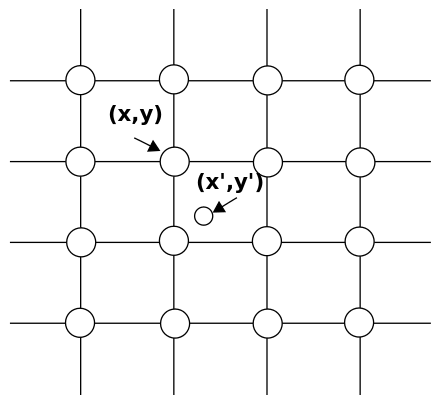
\includegraphics[width=0.9	\textwidth]{./Figures/cap3/convolucionCubica_matriz.png}
		    	\caption{Convoluci\'on c\'ubica.}
		    	\label{fig:convCubica2}
		    \end{figure}
	\end{itemize}


\subsection{Correcci\'on radiom\'etrica}
La correci\'on radiom\'etrica se encarga de minimizar los desajustes producidos en el registro del valor digital en las celdas de la imagen, de hecho en algunos casos las estaciones receptoras llevan a cabo alg\'un tipo de correcci\'on en el momento de recepci\'on de la imagen. La corrección radiom\'etrica implica por una parte la restauraci\'on de lineas o p\'ixeles perdidos y por otra la correcci\'on del bandeado en la imagen \cite{teledUm}.
    \begin{figure}[H]
    	\centering
    	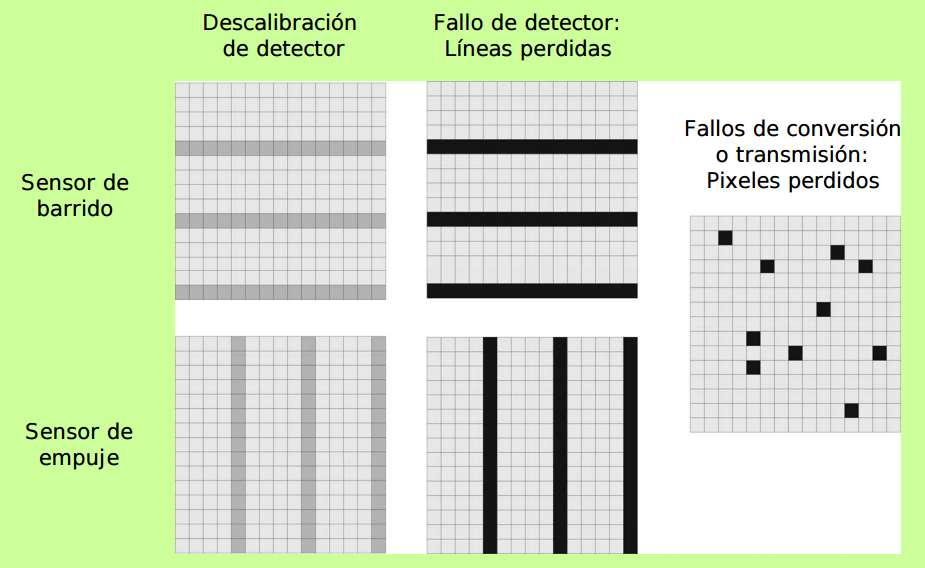
\includegraphics[width=0.9	\textwidth]{./Figures/cap3/correcError.png}
    	\caption{Fallos del sensor en la captura de la imagen.}
    	\label{fig:correcError}
    \end{figure}

\subsubsection{Pixeles o lineas perdidas}\label{subsec:pixelesP}
Si se ha perdido el valor de alg\'un pixel la solución m\'as simple ser\'ia estimarlo como la media de los valores
del mismo pixel en las lineas anterior y posterior (no es recomendable utilizar los pixeles contiguos de la misma linea por que han sido captados por el mismo detector o banda que ha dado el fallo, por tanto son poco fiables).\\~\\
Sea $ f^{'}:(x,y,i)\longrightarrow \{0,...,2^{r}\} $ una funci\'on que corrige los pixeles o lineas perdidas en la coordenadas $ (x,y) $ de la banda $ i $:

		\begin{equation}
		f^{'}(x,y,i) = \ldbrack \dfrac{f(x-1,y,i) + f(x+1,y,i)}{2}) \rdbrack
		\end{equation} 

				\nomenclature[42]{$ \mu $}{Valor de la media.}
				\nomenclature[43]{$ \sigma $}{Desviaci\'on t\'ipica.}
				\nomenclature[44]{$ z $}{Banda de la imagen satelital.}
La bandas de una imagen son de detectores diferentes y est\'an altamente correlacionadas. Sea  $ z $ una banda de la imagen satelital, donde $ z \in [1,k] $, podr\'ia utilizarse el valor del pixel faltante en una banda diferente para mejorar la estimaci\'on:
		\begin{equation}
		f^{'}(x,y,i) = \ldbrack (\dfrac{f(x-1,y,i)-f(x+1,y,i)}{2})+ \dfrac{\sigma_{i}}{\sigma_{z}} +(f(x,y,z)-\dfrac{f(x-1,y,z)-f(x+1,y,z)}{2}) \rdbrack
		\end{equation} 
\nomenclature[45]{$ f^{'}(x,y,i) $}{Nivel digital, con correcci\'on del pixel o linea perdida de las coordenadas $ (x,y) $ en la banda $ i $.}
En caso de que la imagen abarque un territorio amplio y cambiante resulta recomendable calcular las desviaciones t\'ipicas ($ \sigma_{i} $ y $ \sigma_{z} $) en un entorno cercano al pixel perdido.\\~\\
Para detectar lineas perdidas se compara la media de los $ ND $ de una linea con las medias de las lineas anterior y posterior, para detectar pixeles perdidos se compara el valor de un pixel con los de los 8 pixeles.
\subsubsection{Bandeado}\label{subsec:bandeado}
El fen\'omeno del bandeado se debe a una mala calibraci\'on entre detectores y resulta especialmente visible en las zonas de baja radiancia (zonas marinas por ejemplo). El resultado es la aparici\'on peri\'odica de una banda m\'as clara u oscura que las dem\'as.
Para corregir el bandeado se asume que, en caso de no haber error, los histogramas obtenidos por cada uno de los detectores ser\'ian similares entre s\'i y similares al histograma global de la imagen que se toma como referencia.\\~\\
En primer lugar se calculan los coeficientes $ m $ y $ s $ para una correcci\'on lineal de cada uno de las bandas.
		\begin{equation}
		m =\dfrac{\sigma_{i}}{\sigma_{z}}
		\end{equation} 	
				\begin{equation}
				s=\mu_{i} - m\mu_{z}
				\end{equation} 	
				

A continuaci\'on los $ ND $ de la imagen se recalculan a partir de la funcion $ f^{''}:(x,y,i) \longrightarrow \{0,...,2^{r}\} $
				\begin{equation}
				f^{''}(x,y,i) = m f'(x,y,i) + s
				\end{equation} 				
		\nomenclature[46]{$ f^{''}(x,y,i) $}{Nivel digital, con correcci\'on de bandeado, del pixel con coordenadas $ (x,y) $ de la banda $ i $.}

    \begin{figure}[H]
    	\centering
    	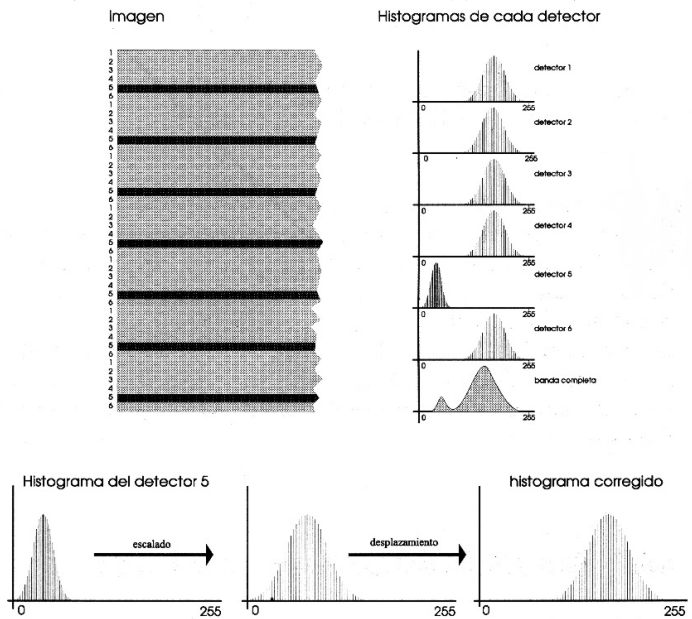
\includegraphics[width=0.9	\textwidth]{./Figures/cap3/bandeo_k.png}
    	\caption{Proceso de correcci\'on del bandeo.}
    	\label{fig:bandeado}
    \end{figure}

\section{Proceso de detecci\'on de cambios}
En los m\'etodos comunes de detecci\'on de cambios se asigna un valor correspondiente al grado de cambio sobre cada celda, independientemente del resto de la imagen. En estos m\'etodos se considera la celda como unidad b\'asica (\'algebra de imagen) para aplicar las correspondientes operaciones matem\'aticas asociadas a cada algoritmo.\\~\\
Los m\'etodos de comparaci\'on, generan una imagen (\'indice de cambios) que representa el grado de cambio entre dos situaciones temporales; las celdas de la imagen resultante, contienen una variable continua de tipo cuantitativo, por lo que se requieren t\'ecnicas que los conviertan en variables cualitativa\cite{martinez2013normalizacion}.
\subsection{Comparaci\'on multitemporal}\label{subsec:compMult}
La comparaci\'on parte de un par de im\'agenes semejantes que abarcan la misma zona de estudio, siguiendo una secuencia multitemporal; cuando los conjuntos de im\'agenes son de car\'acter radiom\'etrico, se recomienda haber aplicado un proceso previo de correcci\'on radiom\'etrica. Singh\cite{singh1989review}, Chuvieco\cite{chuvieco1998factor} y Estornell\cite{estornell2004analisis}, muestran como operaciones más utilizadas:
	\begin{itemize}
		\item \textbf{Diferencia de im\'agenes:} es el m\'etodo m\'as simple, f\'acil de interpretar y directo, ya que consiste en una diferencia algebraica entre los niveles digitales ($ ND $ ) inicial y final para la obtenci\'on de un \'indice ($ I_{dif} $). Normalmente es realizada combinada  con extracciones de \'indices espectrales.
								\begin{equation}
								I_{dif} = ND_{final}-ND_{inicial}
								\end{equation} 	
\nomenclature[47]{$ I_{dif} $}{Indice de cambio por diferencia de im\'agenes.}
\nomenclature[48]{$ I_{ratio} $}{Indice de cambio por el m\'etodo de ratio.}
				\item \textbf{Ratio:} se obtiene aplicando la operación de cociente, entre los niveles digitales ($ ND $ ) inicial y final para la obtenci\'on de un \'indice ($ I_{ratio} $). Podr\'ia  generar mejores resultados pero no se ajusta a una distribución normal.
										\begin{equation}
										I_{ratio} = \dfrac{ND_{final}}{ND_{inicial}}
										\end{equation} 	

		\end{itemize}
Estas dos operaciones generan un \'indice de cambios $ I_{c}$ a partir de cada conjunto de datos multitemporal, dando lugar a tantos mapas de cambios como bandas/capas se consideren; son de gran utilidad cuando se trabaje con im\'agenes pancrom\'aticas o \'indices espectrales/texturales.
\subsection{Criterios de decisi\'on}
La comparaci\'on multitemporal facilita im\'agenes continuas del cambio. En otras palabras, el resultado de los c\'alculos es una imagen en donde el valor de salida indica el grado de cambio, desde la mayor p\'erdida a la mayor ganancia, en una escala gradual. Si se pretende generar una imagen binaria (cambio/estable), es preciso se\~{n}alar un umbral que delimite ambas categor\'ias en las im\'agenes. Ah\'i se plantea un problema de dif\'icil soluci\'on ya que no existen criterios de aplicación general.\\~\\
Si el cambio abarca un sector importante de la imagen, el histograma de la imagen de cambios debiese mostrar un perfil bimodal, lo que permitir\'ia establecer umbrales naturales de cambio, aunque esta situaci\'on no es muy habitual, ya que los cambios en la naturaleza no suelen producirse de modo abrupto\cite{martinez2013normalizacion}.\\~\\
Si es necesario establecer un umbral para separar las \'areas de cambio, puede optarse por se\~{n}alar alg\'un criterio estad\'istico, como la media y la desviaci\'on t\'ipica de una serie de p\'ixeles elegidos aleatoriamente. En ocasiones se ha propuesto utilizar unas \'areas de entrenamiento para calcular que rango de desviaci\'on se pod\'ia considerar l\'imite para p\'ixeles estables, aplicando luego ese valor al conjunto de la imagen\cite{tung1988determination}.

\subsubsection{Discriminaci\'on de las zonas de cambio}\label{sec:discriminacion}
La ecuaci\'on \ref{ec:umbralizacion} genera una m\'ascara binaria de cambios (0, No Cambio; 1, Cambio) aplicando un umbral ($ U $) especifico sobre la imagen resultante del proceso de comparaci\'on multitemporal \cite{singh1989review}. Son f\'acilmente implementables en procesos de car\'acter autom\'atico/semiautom\'atico. Según Estornell \cite{estornell2004analisis}, partiendo de la hip\'otesis de que el porcentaje de cambios es muy reducido, los valores correspondientes se encuentran situados en los extremos del histograma de frecuencias. Para generar una m\'ascara de cambios es preciso se\~{n}alar un umbral que delimite ambas categorías (cambio/no cambio) a partir del \'indice de cambios ($ I_{c} $)\cite{radke2005image}.
Sea $ B:I_{c} \longrightarrow \{0,1\}$ 	una funci\'on que binariza una imagen en base a un Umbral $ U $:
\begin{equation}\label{ec:umbralizacion}
B(I_{c}) = \begin{cases}
1 & \text{si se cumple que } \abs{I_c} \geq U \\
0 & \text{en cualquier otro caso}
\end{cases}
\end{equation}

\nomenclature[49]{$ I_{c} $}{Indice de cambio entre dos im\'agenes.}
\nomenclature[50]{$ B $}{Imagen binaria en el proceso de detecci\'on de cambio.}
\nomenclature[51]{$ B(I_{c}) $}{Nivel digital para el $ I_{c} $.}
\nomenclature[52]{$ U $}{Umbral que binariza una imagen en base a un $ I_{c} $.}

En Rodriguez-Galiano \cite{rodriguez2010analisis} se propone, como criterios de decisi\'on, el m\'etodo de discriminaci\'on basado en los par\'ametros estad\'isticos del \'indice de cambio entre la secuencia temporal de im\'agenes:
\begin{equation}
U=\mu_{I_{c}} \pm n\sigma _{I_{c}}
\end{equation}
\nomenclature[53]{$ n $}{Coeficiente de fiabilidad de los datos.}
\nomenclature[54]{$ \sigma_{I_{c}} $}{Desviaci\'on t\'ipica de la imagen de \'Indices de cambio.}
\nomenclature[55]{$ \mu_{I_{c}} $}{Media de la imagen de \'Indices de cambio.}
Donde, el valor de umbral entre cambio/no cambio $ (U) $ se estima en funci\'on de los par\'ametros estad\'isticos $ (\mu_{I_{c}}, \sigma_{I_{c}}) $ y un coeficiente de tolerancia $ n $ asignado en base a la fiabilidad de los datos. En Estornell \cite{estornell2004analisis} se clasifican los resultados en funci\'on de $ n $; alta probabilidad de cambio $ (n \geq 2) $ y
zonas de media probabilidad de cambio $ (1 < n < 2) $.

\subsection{Filtrado}
Los filtros constituyen unos de los principales m\'etodos del procesamiento digital de im\'agenes . Pueden usarse para distintos fines, pero siempre, el resultado sobre cada pixel depende de los pixeles en su entorno. Tiene como objetivos: 
	\begin{itemize}
		\item \textbf{Suavizar la imagen:} reducir las variaciones de intensidad entre p\'ixeles vecinos.
		\item \textbf{Eliminar ruido:}  modificar aquellos p\'ixeles cuyo nivel de intensidad es muy diferente al de sus vecinos.
		\item \textbf{Realzar la imagen:} aumentar las variaciones de intensidad, all\'i donde se producen.
		\item \textbf{Detectar bordes::} detectar aquellos p\'ixeles donde se produce un cambio brusco en la funci\'on intensidad.	
	\end{itemize}
\subsubsection{Filtro de la mediana}\label{subsec:filMediana}
El filtrado tiene como ventaja de que el valor final del pixel es un valor real presente en la imagen, siendo dicha variable, la mediana entre los niveles digitales pertenecientes a su vecindad. La mediana es el valor para el cual el 50 \% de todos los p\'ixeles en el histograma son mayores y 50 \% son menores, al contrario de la media \'esta no es influenciada por los valores m\'aximos o m\'inimos\cite{mehl1997fundamentos}.

    \begin{figure}[H]
    	\centering
    	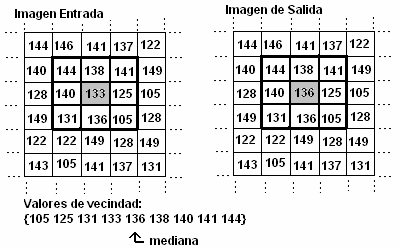
\includegraphics[width=0.8	\textwidth]{./Figures/cap3/FiltrodelaMediana.png}
    	\caption{Proceso del filtro de mediana.}
    	\label{fig:filMediata}
    \end{figure}

\section{Resumen}

La utilizaci\'on de im\'agenes satelitales implica un pre-procesamiento adicional, diferente a las que se le realiza a im\'agenes normales. Estos pre-procesamientos van ligados a resoluciones, firmas espectrales y tipos de im\'agenes satelitales propias del sensor espacial que captura la informaci\'on. En este capitulo se brinda conceptos relacionados a lo descripto en lo anterior, como tambi\'en se describen conocimientos previos para aplicar an\'alisis multitemporales y detecci\'on de cambio en im\'agenes de sat\'elite que componen piezas fundamentales en la metodolog\'ia propuesta.
\newpage{\ } 
\thispagestyle{empty} 

\chapter{Materiales y Metodolog\'ia}
\lhead{Capítulo 4. \emph{Materiales y Metodolog\'ia}} % This is for the header on each page - perhaps a shortened title
En este cap\'itulo se describir\'an los materiales a utilizar en la elaboraci\'on de la metodolog\'ia, as\'i como tambi\'en aquellos a utilizar en las diversas pruebas y validaciones. Adem\'as se presentan las diversas características de las imágenes satelitales a ser empleados en el estudio. La metodolog\'ia nos presenta los diferentes procesos o m\'odulos necesarios para la estimaci\'on de p\'erdida de carbono.
\section{Materiales}
Un grupo de im\'agenes fueron utilizadas para los diferentes estudios y procedimientos de la metodologia, tales como:
\begin{itemize}
	\item Im\'agenes satelitales Landsat.
	\item Im\'agenes Campos Continuos de Vegetación (VCF).
	\item Im\'agen Mapa global de carbono - Paraguay.
	\item Paraguay Forest Change Product.
\end{itemize}
En el procesamiento e implementaci\'on de algoritmos fueron utilizados dos aplicaciones:
\begin{itemize}
	\item GRASS.
	\item Quantum GIS.
\end{itemize}
A continuaci\'on se hablaran con mayor detalle de los elementos citados.
\subsection{Im\'agenes}
En este apartado se pretende brindar las diferentes caracter\'isticas que presentan cada tipo de imagen utilizada en este trabajo..
\subsubsection{Landsat}\label{sec:landsat}
Landsat representa la colecci\'on m\'as larga y continua en el mundo de im\'agenes satelitales con resoluciones moderadas \cite{landsatNasa}. Cuatro d\'ecadas de im\'agenes proporciona un recurso \'unico para personas que trabajan en la agricultura, geolog\'ia, silvicultura, ordenaci\'on territorial, educaci\'on, cartograf\'ia e investigaci\'on del cambio global, como tambi\'en en respuesta de emergencias y operaciones de socorro.\\~\\
Las im\'agenes est\'an disponibles desde 1972 generados por una serie de 6 sat\'elites Landsat. Estos sat\'elites han sido un componente importante del Programa de Observaci\'on de la tierra perteneciente a la NASA, con tres sensores primarios evolucionando a lo largo de treinta años: MSS (Multi-spectral Scanner), TM (Thematic Mapper), y ETM+ (Enhanced Thematic Mapper Plus). 
El 11 de febrero del 2013 fue lanzado el Lansadt 8 correspondiendo al futuro de los sat\'elites Landsat con dos nuevo sensores, Operational Land Imager (OLI) y el Thermal Infrared Sensor (TIRS). La Tabla \ref{t:landsattipos} nos muestra las diferentes resoluciones de los sensores Landsat.

\begin{table}[htb!]
	\centering
	\begin{tabular}{|c|c|c|c|c|c|}
		\hline
		\multirow{2}{*}{\textbf{Landsat}} & \multicolumn{5}{c|}{\textbf{Resoluciones}}                                                             \\ \cline{2-6} 
		& \textbf{Espacial} & \textbf{Espectral} & \textbf{Radiom\'etrica} & \textbf{Temporal} & \textbf{Sensor} \\ \hline
		1                                 & 79x79 m2          & 5 bandas           & 6 bits                  & 18 dias           & MSS             \\ \hline
		2                                 & 79x79 m2          & 5 bandas           & 6 bits                  & 18 dias           & MSS             \\ \hline
		3                                 & 79x79 m2          & 5 bandas           & 6 bits                  & 18 dias           & MSS             \\ \hline
		4                                 & 30x30 m2          & 7 bandas           & 8 bits                  & 16 dias           & TM              \\ \hline
		5                                 & 30x30 m2          & 7 bandas           & 8 bits                  & 16 dias           & TM              \\ \hline
		6                                 & 30x30 m2          & 8 bandas           & 8 bits                  & 16 dias           & ETM+            \\ \hline
		7                                 & 30x30 m2          & 8 bandas           & 8 bits                  & 16 dias           & ETM+            \\ \hline
		8                                 & 30x30 m2          & 9 bandas           & 12 bits                 & 16 dias           & OLI/TIRS        \\ \hline
	\end{tabular}
	\caption{Resoluciones de los sat\'elites Landsat.}
		\label{t:landsattipos}
\end{table}
El Sistema de Referencia Mundial Landsat-2 (WRS-2: Landsat Worldwide Reference System-2) provee un esquema de indexaci\'on para el patr\'on de repetici\'on de la trayectoria orbital terrestre seguida por las plataformas espaciales Landsat 4, 5 y 7 sobre los 16 d\'ias de su repetitivo ciclo orbital \cite{els2015refere}. El original WRS (WRS-1) fue dise\~{n}ado para las misiones Landsat 1, 2, y 3, las cuales se movieron en una \'orbita m\'as alta. El actual WRS-2 fue dise\~{n}ado para la \'orbita a 705 Km usada para las \'ultimas misiones. En la Figura \ref{fig:wrs2Image} podemos observar los \'indices (Path y Row) en el momento de la obtenci\'on de una imagen satelital Landsat para una zona.

\begin{figure}[H]
	\centering
	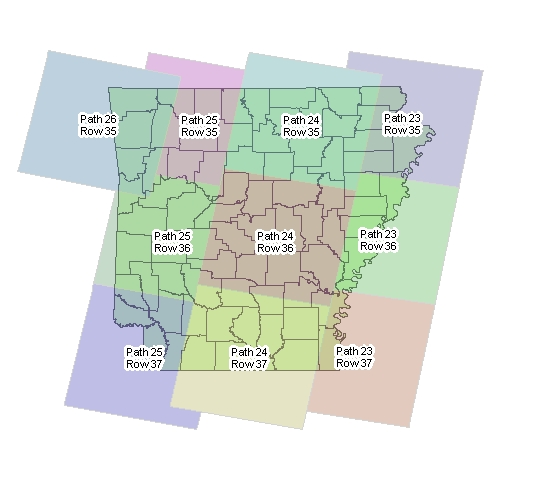
\includegraphics[width=0.8	\textwidth]{./Figures/cap4/wrs2_22.jpg}
	\caption{Ejemplo WRS-2 Path/Row}
	\label{fig:wrs2Image}
\end{figure}

El Servicio Geol\'ogico de los Estados Unidos (USGS) es una agencia cient\'ifica de los Estados Unidos, el cual proveen un producto llamado L1T (Level 1 Terrain Corrected) que implica las im\'agenes Landsat con datos pre-procesados para una correcci\'on radiom\'etrica sistem\'atica y correcci\'on geom\'etrica mediante la incorporaci\'on de puntos de control en tierra. Estos productos est\'an en la Web de forma gratuita \cite{landsatNasa}.


\subsubsection{Campos Continuos de Vegetación (VCF)}\label{sec:vcf}
Las im\'agenes VCF contienen estimaciones proporcionales para los tipos de cobertura vegetal: vegetaci\'on le\~{n}osa, vegetaci\'on herb\'acea y suelo desnudo. El producto se deriva de las siete bandas del sensor MODerate-resolution Imaging Spectroradiometer (MODIS) a bordo del sat\'elite Terra, perteneciente a la NASA. El esquema de clasificaci\'on continuo del VCF puede representar \'areas terrestres heterog\'eneas mejor que los esquemas tradicionales de clasificaci\'on discreta. Los sistemas de clasificaci\'on tradicionales indican donde se concentran los tipos de cobertura del suelo. El VCF posee un resoluci\'on espacial de 250x250 metros cuadrados y la colecci\'on de im\'agenes se encuentra disponible gratuitamente en la Web \cite{gl2015Uni}.
La Figura \ref{fig:vcfImage} nos presenta un imagen, con diferentes tonalidades de color, para los porcentajes de vegetaci\'on y los niveles digitales del agua como pixeles nulos.
\begin{figure}[H]
	\centering
	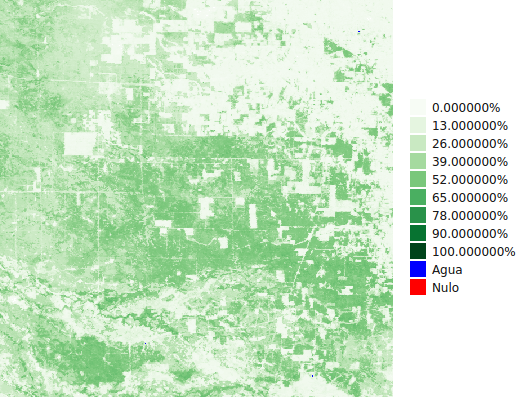
\includegraphics[width=0.8	\textwidth]{./Figures/cap4/vcf_image.png}
	\caption{Imagen VCF con diferentes tonalidades de color de acuerdo al porcentaje de vegetaci\'on.}
	\label{fig:vcfImage}
\end{figure}
\subsubsection{Mapa global de carbono - Paraguay}\label{sec:saatchiMapa}
El mapa global de carbono \cite{saatchi2011benchmark} nos provee la densidad de carbono, expresada en toneladas de carbono por hect\'area, del \'area ocupada por un pixel. El mapa fue elaborado para la d\'ecada de los 2000. En la actualidad existen diferentes mapas de carbono a nivel mundial \cite{saatchi2011benchmark}. La Figura \ref{fig:saatchi} representa el mapa global de carbono disponible para el Paraguay.
\begin{figure}[H]
	\centering
	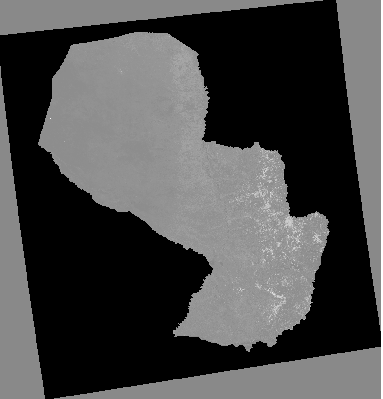
\includegraphics[width=0.8	\textwidth]{./Figures/cap5/saatchi.png}
	\caption{Mapa Global de Carbono - Paraguay}
	\label{fig:saatchi}
\end{figure}


\subsubsection{Paraguay Forest Change Product}\label{sec:fcc}
El Paraguay Forest Change Product (PFCP) muestra donde ocurri\'o la deforestaci\'on en Paraguay durante 1990-2000. El PFCP fue elaborado a partir de las im\'agenes Landsat TM y ETM+, identificando seis clases; bosque atl\'antico, Chaco bosques, el agua, no forestales y la deforestaci\'on. El producto puede ser utilizado para determinar procesos y patrones de cambio en la cubierta forestal. En la Figura \ref{fig:fcc} se puede observar el PFCP (disponible gratuitamente \cite{gl2015Uni}). En la Tabla \ref{t:pfcptab} se describe la representaci\'on de cada nivel digital en dicha imagen. .
\begin{table}[htbp]\centering
\begin{tabular}{|c|c|c|}
	\hline \textbf{Valor digital} &\textbf{ Representaci\'on} & \textbf{Color sugerido} \\ 
	\hline 1 & Bosque Atl\'antico & Verde \\ 
	\hline 2 & Bosque Chaque\~{n}o & Verde Claro \\ 
	\hline 3 & No Bosque & Agua \\ 
	\hline 4 & Agua & Azul \\ 
	\hline 5 & P\'erdida Bosque Atl\'antico & Rojo \\ 
	\hline 6 & P\'erdida Bosque Chaque\~{n}o & Purpura Claro \\ 
	\hline 
\end{tabular} 
\caption{Representaci\'on del valor digital en la imagen PFCP.}
\label{t:pfcptab}
\end{table}

\begin{figure}[H]
	\centering
	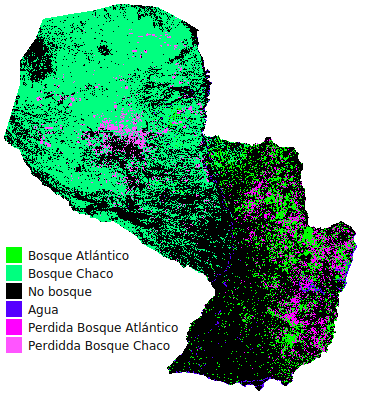
\includegraphics[width=0.7	\textwidth]{./Figures/cap4/fcc_paraguay.png}
	\caption{Paraguay Forest Change Product}
	\label{fig:fcc}
\end{figure}



\subsection{Aplicaciones}
Sistemas de informaci\'on geogr\'afica fueron utilizados para la manipulaci\'on de im\'agenes satelitales, como tambi\'en para dise\~{n}ar e implementar los algoritmos utilizados en la metodolog\'ia propuesta. A continuaci\'on se describen las aplicaciones utilizadas.

\begin{itemize}
	\item \textbf{GRASS: }es un software SIG  bajo licencia GPL (software libre) \cite{osgeoGrass}. El software soporta informaci\'on tanto raster como vectorial y posee herramientas de procesado digital de im\'agenes. Esta disponibles principalmente para plataformas Linux.
	\item \textbf{Quantum GIS: }es un SIG de c\'odigo libre para plataformas GNU/Linux, Unix, Mac OS, Microsoft Windows y Android. La principal diferencia con el GRASS es la interfaz amigable con que cuenta y la facilidad de integraci\'on con nuevas funciones espaciales desarrollados por los usuarios \cite{qgisSIG}.
\end{itemize}

\section{Metodolog\'ia}
Los datos de entrada son las im\'agenes Landsat pre-procesadas (correcciones geom\'etricas y radiom\'etricas) de manera a disminuir los errores de localizaci\'on e intensidad de los niveles digitales causados por distintos factores (secci\'on \ref{sec:correcionesImages}).  
Las im\'agenes Landsat 8 no deben ser mezcladas con im\'agenes de otro sensor del mismo sat\'elite, ya que esta posee una resoluci\'on radiom\'etrica de 16 bits y las dem\'as son capturadas a 8 bits. Las bandas utilizadas corresponde a la infrarroja cercana y roja.\\~\\
En la Figura \ref{fig:metodologiapc} podemos observar que a partir de las banda infrarroja cercana y roja ($ f_{t}(x,y,IRc);f_{t}(x,y,R) $, $ f_{t_{*}}(x,y,IRc);f_{t_{*}}(x,y,R) $) de una secuencia multitemporal, donde $ t < t_{*} $, es posible obtener una mascara de perdida forestal $ MPF $ y su cuantificaci\'on ($ CCP $) en toneladas de carbono perdidos ($ ton $ $ C $) una vez pasado por los procesos de detecci\'on de cambio forestal y estimaci\'on de p\'erdida de carbono Forestal.
\begin{figure}[H]
	\centering
	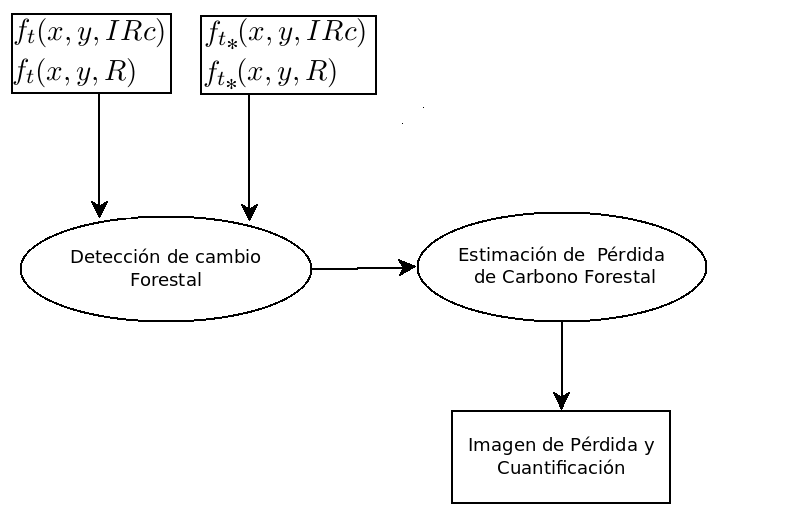
\includegraphics[width=0.8	\textwidth]{./Figures/cap4/metodologiaCarbono_3.png}
	\caption{Diagrama de flujo. Metodolog\'ia propuesta}
	\label{fig:metodologiapc}
\end{figure}

\subsection{Detecci\'on de cambio Forestal}
La detecci\'on de cambio cumple un papel fundamental en la metodolog\'ia ya que nos permite categorizar el cambio en la secuencia temporal estudiada. Este proceso presenta una metodolog\'ia automatizada a trav\'es del calculo de par\'ametros estad\'isticos extra\'ido de las im\'agenes satelitales y el uso de variables determinadas en un previo an\'alisis del comportamiento espectral observados en la cobertura vegetal de prueba.

\subsubsection{Detecci\'on de cambio}
En este proceso se detecta el cambio entre dos tiempos de im\'agenes satelitales. El resultado esperado constituye una mascara de perdida ($ MP $) entre las series temporales de im\'agenes comparadas. 
\paragraph{Comparaci\'on Multitemporal}\mbox{}\\\mbox{}\\
El siguiente paso despu\'es de haber equiparado radiom\'etricamente (secci\'on \ref{sec:capNormalizacion}) las im\'agenes consiste en la comparaci\'on multitemporal, permitiendo obtener un indice de cambio (variable cuantitativa) en cada pixel resultante. El m\'etodo de diferencia de im\'agenes es utilizada debido a que el m\'etodo Ratio no se ajusta a una distribuci\'on normal, se asume que el cambio es reducido y por ende est\'an ubicados hacia los extremos del histograma de la imagen con los \'indices de cambio $ I_{c} $, condici\'on clave para la umbralizaci\'on estad\'istica. La comparaci\'on es realizado sobre la imagen con los NDVI de cada serie temporal a modo a resaltar la vegetaci\'on y simplificar la cantidad de bandas utilizadas, observando a su vez que los datos estables ser\'an pr\'oximos a $ 0 $ gracias a la semejanza existente entre los pixeles. 
\paragraph{Umbral estad\'istico} \label{sec:umbralEstadistico2}\mbox{}\\\mbox{}\\
Los criterios de decisi\'on propuesto en la secci\'on \ref{sec:discriminacion} asignan valores de cambio/no cambio en funci\'on a un umbral. Estos criterios permiten convertir los indices de cambios a valores cualitativos que representan una m\'ascara de cambio ($ MC $). El m\'etodo basados en par\'ametros estad\'isticos es escogido por su sencillez y coherencia con el m\'etodo de comparaci\'on multitemporal aplicada. Los niveles digitales de $ MC $ est\'an definidos por la siguiente expresi\'on:
\begin{equation}\label{ec:umbMetodo}
MC(x,y) = \begin{cases}
1 & \text{si se cumple que } \mu_{I_{c}} - n \times \sigma_{I_{c}} < I_{c}(x,y) < \mu_{I_{c}} + n \times \sigma_{I_{c}}\\
0 & \text{cualquier otro caso}  
\end{cases}
\end{equation}
En la Figura \ref{fig:umbrales} se puede observar una linea roja y verde, que determinan los limites para los cuales los \'indices no son considerados pixeles de cambio (pixeles que no variaron con respecto al tiempo). La variable de fiabilidad $ n $ es elegida en base a la probabilidad de cambio deseado para la detecci\'on (secci\'on \ref{sec:discriminacion}).
	\begin{figure}[H]
		\centering
		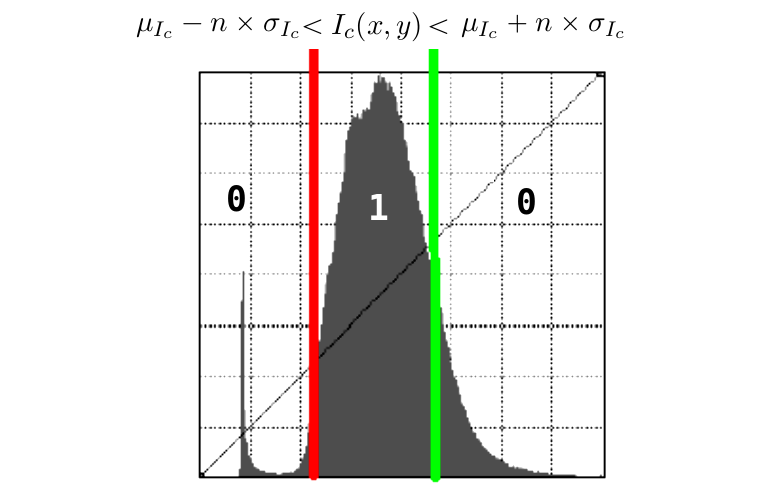
\includegraphics[width=0.8	\textwidth]{./Figures/cap4/umbrales_3.png}
		\caption{Umbrales que binarizan los indices de cambios $ I_{c} $.}
		\label{fig:umbrales}
	\end{figure}
Los pixeles que sufrieron perdida estar\'an definidos por una m\'ascara $ MP $ con las siguiente expresi\'on:
\begin{equation}\label{ec:umbMetodoMP}
MP(x,y) = \begin{cases}
1 & \text{si se cumple que } I_{c}(x,y) < \mu_{I_{c}} - n \times \sigma_{I_{c}} \\
0 & \text{cualquier otro caso}  
\end{cases}
\end{equation}
\paragraph{Iteraci\'on}\label{subsec:iteracion}\mbox{}\\\mbox{}\\
 Si dos im\'agenes se consideran semejantes, los cambios producidos en el terreno afectan a la radiometr\'ia registrada en las im\'agenes, y por tanto, en los par\'ametros estad\'isticos que las definen.\\~\\
En la normalizaci\'on radiom\'etrica los cambios introducen ruido \cite{martinez2013normalizacion}, ya que el proceso busca que los pixeles de una banda de im\'agenes satelitales en diferentes tiempos sean semejantes y el cambio estar\'ia influyendo en la correlaci\'on entre los pixeles que verdaderamente no sufrieron cambio. Si el \'area de todos los pixeles con cambio es mayor, la influencia en la normalizaci\'on ser\'a mayor y por ende afectara la precisi\'on en la detecci\'on de cambios. En vista al problema, mediante una normalizaci\'on radiom\'etrica iterativa se pretende minimizar dicha influencia, donde los par\'ametros estad\'isticos ($ \mu,\sigma $) utilizados constituyen los pixeles sin cambios.\\~\\	
La Figura \ref{fig:deteccionCambio} nos presenta el ciclo de procedimientos para la detecci\'on de cambio, donde a partir de la secuencia de im\'agenes satelitales en las bandas infrarroja cercana y roja ($ f_{t}(x,y,IRc);f_{t}(x,y,R), f_{t_{*}}(x,y,IRc);f_{t*}(x,y,R) $) son calculados los par\'ametros estad\'isticos ($ \mu_{i,t};\sigma_{i,t}, \mu_{i,t_{*}};\sigma_{i,t_{*}} $) para las im\'agenes. Esos par\'ametros son utilizados para normalizar radiom\'etricamente las bandas del tiempo $ t_{*} $, en semejanza a las bandas de la imagen satelital del tiempo $ t $, as\'i determinar la imagen con los \'indices de cambios ($ I_{c} $) una vez calculados los NDVI ($ ndvi_{f_{t}},ndvi_{f_{t_{*}}} $). La m\'ascara de cambio ($ MC $) es el resultado de pasar por los umbrales estad\'isticos (secci\'on \ref{sec:umbralEstadistico2}). La iteraci\'on ($ iter $) continua si la media del $ I_{c} $ actual es de magnitud similar a la registrada en la anterior. Se define la función l\'ogica $ continuar $:
  \begin{equation}\label{ec:continuar}
  continuar(\mu_{I_{c}^{iter}},\mu_{I_{c}^{iter-1}}) = \begin{cases}
  falso & \text{si se cumple que } \mu_{I_{c}^{iter}} - \mu_{I_{c}^{iter-1}} \leq \epsilon \\
  verdadero & \text{en cualquier otro caso }
  \end{cases}
  \end{equation}
  \nomenclature[58]{$ \epsilon $}{Error de cambio.}
  Siendo $ \epsilon $ un error de aproximaci\'on. Si el proceso de iteraci\'on debe continuar, el c\'alculo  de los par\'ametros estad\'isticos debe realizarse seg\'un el Algoritmo \ref{alg:parametros}. Cada valor de pixel, de las bandas en cada imagen satelital, es utilizado en el c\'alculo si no representa un cambio en la m\'ascara de cambio $ MC $.
  \begin{algorithm}[H]
  	\caption{Funci\'on que calcula los par\'ametros estad\'isticos.}
  	\label{alg:parametros}
  	\begin{algorithmic}[1]
  		\Statex
  		\Function {parametros}{$f_{t}(x,y,R),f_{t}(x,y,IRc),MC$}
		\State $sumR =0$ \Comment{Variable auxiliar sumatoria}
		\State $sumIRc =0 $ \Comment{Variable auxiliar sumatoria}
		\State $nT =0 $ \Comment{N\'umero de pixeles sin cambio}
		\Statex
		\For {$x \gets 0, fil$}
			\For {$y \gets 0, col$}
%															\algstore{myalg2}
%														\end{algorithmic}
%													\end{algorithm}
													
%													\begin{algorithm}                     
%														\begin{algorithmic} [1]                   % enter the algorithmic environment
%															\algrestore{myalg2}
				\If{$MC(x,y)=1$}
					\State $sumR=sumR+f_{t}(x,y,R)$
					\State $sumIRc=sumIRc+f_{t}(x,y,IRc)$
					\State $nT=nT++$
				\EndIf
			\EndFor
		\EndFor
	\Statex
		\State $ \mu_{R,t}= sumR/nT$
		\State $ \mu_{IRc,t}= sumIRc/nT$
		\State $ sumR=0$
		\State $ sumIRc=0$
		\Statex
		\For {$x \gets 0, fil$}
			\For {$y \gets 0, col$}
				\If{$MC(x,y)=1$}
					\State $sumR=sumR+(f_{t}(x,y,R)-\mu_{R,t})^{2}$
					\State $sumIRc=sumIRc+(f_{t}(x,y,IRc)-\mu_{IRc,t})^{2}$
				\EndIf
			\EndFor
		\EndFor
		\Statex
		\State $\sigma_{R,t}=\sqrt{\dfrac{1}{nT-1} \times sumR}$
		\State $\sigma_{IRc,t}=\sqrt{\dfrac{1}{nT-1} \times sumIRc}$
  		\Statex
  		\Return $[\mu_{R,t},\mu_{IRc,t},\sigma_{R,t},\sigma_{IRc,t}]$
  		\EndFunction
  	\end{algorithmic}
  \end{algorithm}
El proceso de iteraci\'on finaliza retornando una un m\'ascara de perdida $ MP $ seg\'un la ecuaci\'on \ref{ec:umbMetodoMP}.\\~\\
\begin{figure}[H]
	\centering
	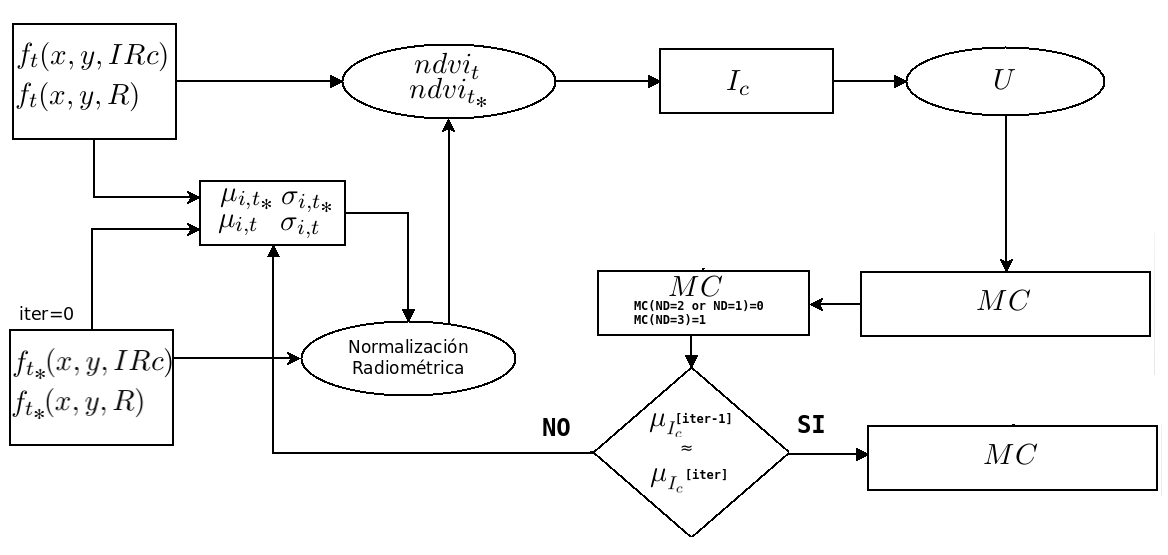
\includegraphics[width=1.0 \textwidth]{./Figures/cap4/deteccionCambio_4.png}
	\caption{Diagrama de flujo. Detecci\'on de Cambio.}
	\label{fig:deteccionCambio}
\end{figure}

En la Figura \ref{fig:iteracionRadiometrica} podemos observar que a partir de la mascara de cambio obtenido en la primera iteraci\'on, los par\'ametros estad\'isticos para la iteraci\'on 2, en la normalizaci\'on iterativa, son realizados sobre los pixeles que no detectaron cambios. 
\begin{figure}[H]
	\centering
	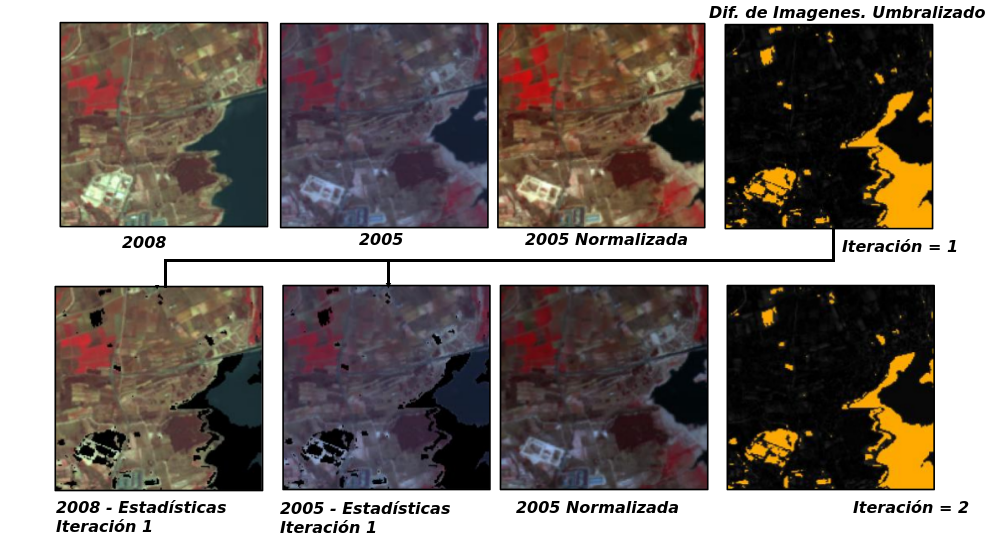
\includegraphics[width=1.0	\textwidth, height=0.5 \textheight]{./Figures/cap4/iteracionUmbra.png}
	\caption{Mascaras de cambio, iteraci\'on de la normalizaci\'on radiom\'etrica.}
	\label{fig:iteracionRadiometrica}
\end{figure}


\subsubsection{Discriminaci\'on Forestal}\label{sec:discrForestalMet}
Las im\'agenes procesadas son aquellas obtenidas en la ultima normalizaci\'on radiom\'etrica, generada por el proceso iterativo y la imagen base para la semejanza en ese proceso. En este procedimiento se busca generar una mascara de vegetaci\'on (MV) de la secuencia temporal.
\paragraph{NDVI}\mbox{}\\\mbox{}\\
El NDVI es calculado para ambas fechas pertenecientes a la secuencia multitemporal evaluada ($ndvi_{f_{t}},ndvi_{f_{t_{*}}}  $). El calculo es hecho teniendo como entradas las bandas infrarroja cercana y roja, donde el vigor vegetal de cada p\'ixel sera determinado por la ecuaci\'on \ref{e:ndvi}. 
\paragraph{Umbral de Vegetaci\'on}\label{sec:uvegetacion}\mbox{}\\\mbox{}\\
El umbral que binariza la vegetaci\'on es determinado a partir de una constante calculada por un previo an\'alisis del comportamiento espectral de la cobertura vegetal y las im\'agenes de NDVI, retornando una imagen binarizada $ ndvi_{f_{t}}^{B} $ dado un $ ndvi_{f_{t}} $. Dicha variable corresponde a la desviaci\'on observada $(\sigma_{c}) $ en la intersecci\'on de puntos de muestreo aleatorios entre im\'agenes VCF y Landsat (secci\'on \ref{subsec:umbralVegetacion}). La ecuaci\'on que determina a $ ndvi_{f_{t}}^{B} $ tiene la siguiente expresi\'on:
  \begin{equation}\label{ec:umbVegetacion}
  ndvi_{f_{t}}^{B}(x,y) = \begin{cases}
  1 & \text{si se cumple que } ndvi_{f_{t}}(x,y) > \mu_{ndvi_{f_{t}}}-n \times \sigma_{c}  \\
  0 & \text{en cualquier otro caso }
  \end{cases}
  \end{equation}
\nomenclature[58]{$ \sigma_{c} $}{Desviaci\'on determinada como constante para la umbralizaci\'on de la cobertura vegetal.}
Donde $ \mu_{ndvi_{f_{t}}} $ representa la media de la imagen $ ndvi_{f_{t}} $ y $ n $ el coeficiente de fiabilidad. En la Figura \ref{fig:ndviUmbral} podemos observar que el umbral del NDVI (linea roja) se situ\'a por debajo de la media (linea fucsia) permiti\'endonos discriminar los pixeles que representan vegetaci\'on/no vegetaci\'on.
\begin{figure}[H]
	\centering
	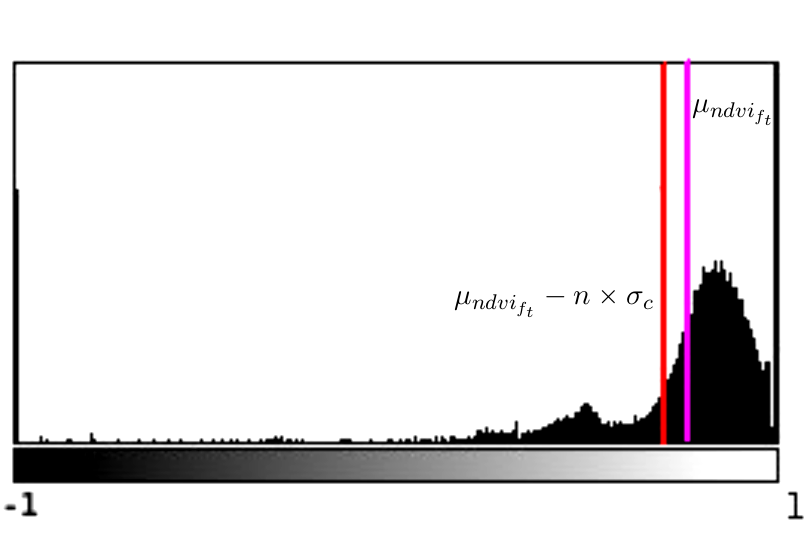
\includegraphics[width=0.8	\textwidth]{./Figures/cap4/ndviUmbral_2.png}
	\caption{Umbral utilizado y la media en el histograma de la imagen con NDVI.}
	\label{fig:ndviUmbral}
\end{figure}

\paragraph{Intersecci\'on \'area boscosa }\mbox{}\\\mbox{}\\
El procedimiento que sigue una vez obtenido los NDVI de las dos fechas es determinar los pixeles que ser\'an evaluados para detectar el cambio, por ello aplicamos una simple operaci\'on de uni\'on ($ ndvi_{f_{t}}^{B} $ OR $ ndvi_{f_{t_{*}}}^{B}$) que generara una mascara de vegetaci\'on $ MV $ correspondiente a los dos tiempos. La Figura \ref{fig:discrimForestal} refleja los pasos realizados para obtener una mascara de vegetaci\'on.
\begin{figure}[H]
	\centering
	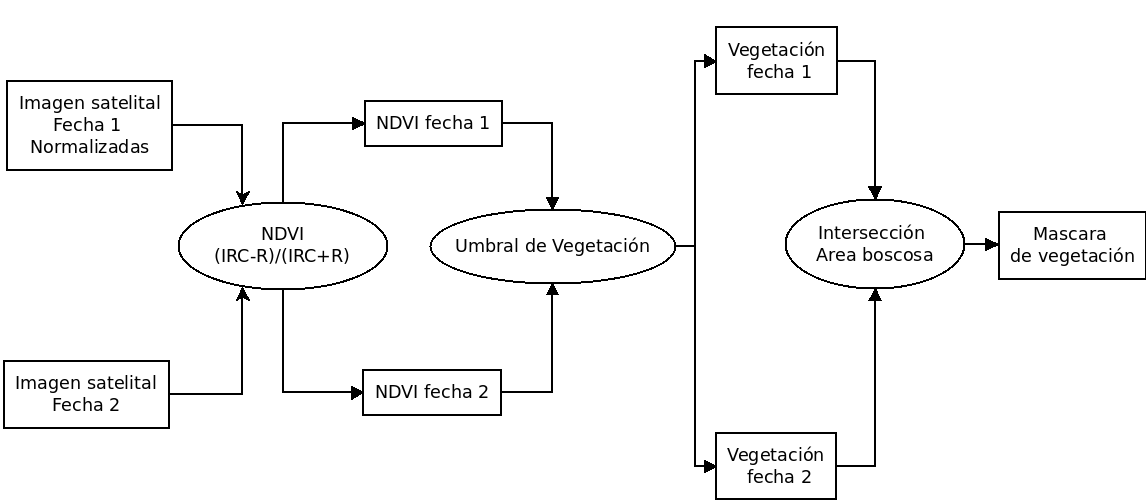
\includegraphics[width=1.0	\textwidth]{./Figures/cap4/discriminacionForestal_2.png}
	\caption{Diagrama de flujo. Discriminaci\'on Forestal.}
	\label{fig:discrimForestal}
\end{figure}


\subsubsection{Mascara de P\'erdida Forestal}
El proceso consiste en la intersecci\'on entre la mascaras de vegetaci\'on y cambio. En la intersecci\'on solo son considerados los cambios correspondiente a p\'erdidas  $ MP $, debido a que se pretende generar una imagen binaria $ MPF $ que represente la perdida forestal en un pixel.\\~\\
La imagen $ MPF $ probablemente tendr\'a errores que son inherentes a los procesos utilizados para su creación \cite{lovell2001filtering}. Estos errores lo consideramos como ruidos en la imagen $ MPF $. El filtro de mediana \cite{gonzalez2002woods} reducir\'a el porcentaje de falsas alarmas en la imagen $ MPF $ eliminando los ruidos generados.
En la Figura \ref{fig:intersPerdida} podemos observar el flujo de tareas para la obtenci\'on de la mascara que representa la perdida forestal en dos tiempos .
\begin{figure}[H]
	\centering
	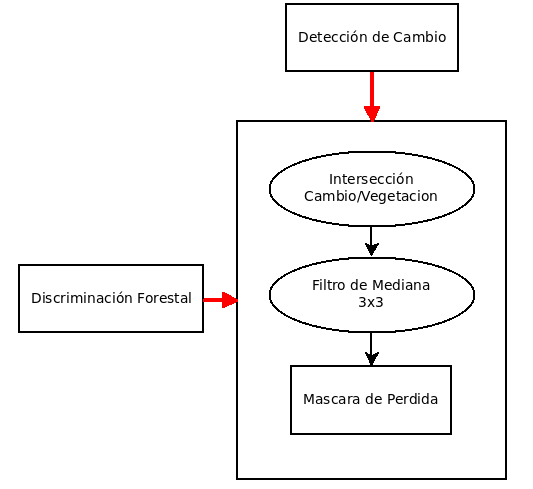
\includegraphics[width=0.6	\textwidth]{./Figures/cap4/interseccionPerdida.png}
	\caption{Diagrama de procedimientos para la obtenci\'on de la m\'ascara de perdida forestal.}
	\label{fig:intersPerdida}
\end{figure}

\subsection{Estimaci\'on de p\'erdida de carbono forestal}
El procedimiento final en la metodolog\'ia consiste en estimar el carbono perdido o no secuestrados dentro del tiempo transcurrido entre las im\'agenes satelitales. El producto constituye la mascara de perdida forestal ($ MPF $) junto con la cuantificaci\'on ($ CCP $) en toneladas de carbono obtenida a trav\'es de una ecuaci\'on de regresi\'on lineal. La ecuaci\'on de regresi\'on fue generada por medio del mapa global de carbono (variable dependiente) \cite{saatchi2011benchmark} y el NDVI (variable independiente) determinadas por las im\'agenes Landsat en un an\'alisis previo (m\'as detalles en la secci\'on \ref{subsec:estimacionCarbono}). La regresi\'on fue evaluada a trav\'es del coeficiente de determinaci\'on $ r^{2} $. En la Tabla \ref{t:coefDeter} se presenta el tipo de relaci\'on del coeficiente de determinaci\'on \cite{kris2014estimacionCorr}.
\nomenclature[59]{$ r^{2}$}{Coeficiente de determinaci\'on para una regresi\'on.}
\begin{table}[H]
	\centering
	\begin{tabular}{|l|l|}
		\hline
		\textbf{Valor} & \textbf{Significado} \\ \hline
		0,0            & Ninguna Relaci\'on     \\ \hline
		0,25           & Relaci\'on baja        \\ \hline
		0,50           & Relaci\'on Moderada    \\ \hline
		0,75           & Relaci\'on Buena       \\ \hline
		1,00           & Relaci\'on perfecta    \\ \hline
	\end{tabular}
	\caption{Rangos del coeficiente de determinaci\'on.}
	\label{t:coefDeter}
\end{table}

Sea $ C:(x,y) \longrightarrow \{ [-\infty,\infty]\}$ la cantidad de carbono, en toneladas por hect\'area, para la coordenada $ (x,y) $, se tiene que: 
\begin{equation}\label{ec:regreLinelCarb}
C(x,y)=h+m \times ndvi_{f}(x,y)
\end{equation}
\nomenclature[59]{$ m$}{Coeficiente en la ecuaci\'on de estimaci\'on de carbono.}
\nomenclature[59]{$ h$}{Coeficiente en la ecuaci\'on de estimaci\'on de carbono.}
Donde $ ndvi_{f} $ representa la variable independiente, $ C $ la variable dependiente y ($ h , m $) coeficientes de la ecuaci\'on de regresi\'on lineal. \\~\\
La estimaci\'on de carbono para una secuencia multitemporal ($ C_{t},C_{t_{*}} $) en funci\'on al ndvi ($ ndvi_{t},ndvi_{t_{*}} $) queda definida de la siguiente manera:
\begin{equation}
\label{e:fecha1m}
C_{t}(x,y)=h+m \times ndvi_{f_{t}}(x,y)
\end{equation}
\begin{equation}
\label{e:fecha2m}
C_{t_{*}}(x,y)=h+m \times ndvi_{f_{t_{*}}}(x,y)
\end{equation}
 El \'indice de cambio generado en la detecci\'on de cambio simplificar\'ia los c\'alculos a la hora de estimar la perdida, ya que:
 \begin{equation}
 \label{e:indiceCambiom}
 Ic(x,y)=ndvi_{f_{t}}(x,y) - ndvi_{f_{t_{*}}}(x,y)
 \end{equation}		
 Podr\'iamos restar la ecuaci\'on \ref{e:fecha1m} y \ref{e:fecha2m}:
 \begin{equation}
 \label{e:restaCarm}
C_{t}(x,y) - C_{t_{*}}(x,y)= m \times (ndvi_{f_{t}}(x,y) - ndvi_{f_{t_{*}}}(x,y))
 \end{equation}		
 \begin{equation}
 \label{e:perdidaCarm}
 PC(x,y)= C_{t}(x,y) - C_{t_{*}}(x,y)
 \end{equation}		
 Siendo $ PC(x,y)$ toneladas de carbono por hect\'area perdidos en un pixel con coordenadas $ (x,y) $. Remplazando \ref{e:indiceCambiom} y \ref{e:perdidaCarm} en \ref{e:restaCarm}, la ecuaci\'on de regresi\'on final quedar\'ia:
 \begin{equation}\label{ec:carbonom}
 PC(x,y) = m \times Ic(x,y)
 \end{equation}
 La ecuaci\'on \ref{ec:carbonom} debe ser multiplicada por un factor de $ 0,09 $, debido a que los pixeles del mapa global de carbono representan toneladas de carbono por hect\'area \cite{saatchi2011benchmark} y la superficie m\'inima representada por las im\'agenes Landsat (utilizadas para el calculo de NDVI) es de $ 900$  $m^{2}=0.09 $  $has. $. La ecuaci\'on final quedar\'ia:
 \begin{equation}\label{ec:carbonoFinalm}
 PC(x,y) = 0.09 \times m \times Ic(x,y)
 \end{equation}
 Siendo la cantidad de carbono perdido (en toneladas de $ C $) representado por la siguiente expresi\'on:
 \begin{equation}\label{ec:carbonoFinalsumatoriam}
 CCP = \Sigma_{c=0}^{fil}\Sigma_{d=0}^{col} PC(x,y)
 \end{equation}
  

 \nomenclature[63]{$PC(x,y)$}{Toneladas de carbono por hect\'area perdidos en las coordenadas $ (x,y) $.}
\nomenclature[60]{$ C(x,y)$}{Toneladas de carbono por hect\'area en las coordenadas $ (x,y) $.}

La ecuaci\'on  \ref{ec:carbonoFinalsumatoriam} ser\'a realizado teniendo en cuenta la m\'ascara de perdida forestal, es decir solo ser\'an sumados aquellos pixeles que representa una perdida seg\'un $ MPF $. La Figura \ref{fig:resulPC} nos muestra el resultado esperado por la metodolog\'ia ($ MPF $ y $ CCP $ ), donde los pixeles de color rojo representa perdida de carbono forestal y los grises a pixeles en las cuales no hubo perdida.
\begin{figure}[H]
	\centering
	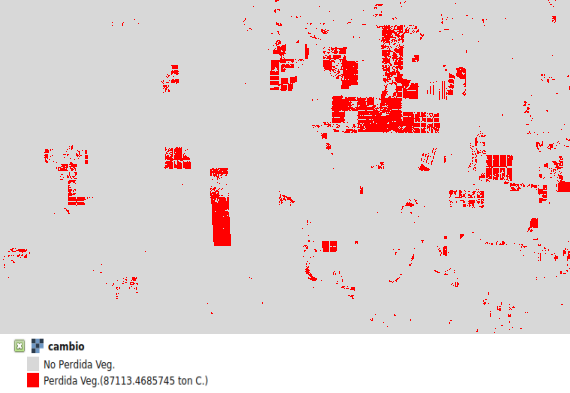
\includegraphics[width=0.8	\textwidth]{./Figures/cap4/resultadoMetodologia.png}
	\caption{Presentaci\'on del resultado. Mascara de perdida Forestal y la cantidad de carbono perdido.}
	\label{fig:resulPC}
\end{figure}
\subsection{Esquema general de la metodolog\'ia}
La metodolog\'ia presenta un esquema general descripta por el Algoritmo \ref{alg1}, desde los datos de entrada hasta su finalizaci\'on, de manera a brindar un resumen de los procesos realizados como también su aplicaci\'on en un ejemplo gr\'afico.
\begin{algorithm}
	\caption{Metodolog\'ia para estimar p\'erdida de carbono}
	\label{alg1}
	\begin{algorithmic}[1]
		\Require {$f_{t}(x,y,IRc);f_{t}(x,y,R), f_{t_{*}}(x,y,IRc);f_{t*}(x,y,R)$}
		\Statex
		\State $ I_{c_{fil \times col}}=  \begin{bmatrix}
		0 & \cdots & 0 \\
		\vdots & \ddots &  \vdots \\
		0 & \cdots & 0
		\end{bmatrix} $ \Comment{Indice de cambio $ I_{c} $}
		\State $ MC_{fil \times col} = \begin{bmatrix}
		1 & \cdots & 1 \\
		\vdots & \ddots &  \vdots \\
		1 & \cdots & 1
		\end{bmatrix} $ \Comment{Mascara de cambio $MC$}
		\State $ seguir = verdadero $ \Comment{Variable que controla la iterac\'on}
		\State $\mu_{anterior} =0$ \Comment{Media de $ I_{c} $ en la iteraci\'on anterior}
		\Statex
		\State $ iter = 0 $
		\While{$seguir$}
		
			\State \Comment{Se calculan las medias y desviaciones en funci\'on a una m\'ascara si no es la}
			\State \Comment{primera iteraci\'on (algoritmo \ref{alg:parametros})}
			\State $[\mu_{R,t},\mu_{IRc,t},\sigma_{R,t},\sigma_{IRc,t}] = \textsc{parametros}(f_{t}(x,y,R),f_{t}(x,y,IRc),MC)$		
			\State $[\mu_{R,t_{*}},\mu_{IRc,t_{*}},\sigma_{R,t_{*}},\sigma_{IRc,t_{*}}] = \textsc{parametros}(f_{t_{*}}(x,y,R),f_{t_{*}}(x,y,IRc),MC)$
			\Statex
			\State \Comment{Utilizar ecuaci\'on \ref{ec:normalizacion} para normalizar}
			\State $f_{t_{*}}^{Norm}(x,y,R) = \textsc{normalizar}(\mu_{R,t_{*}},\sigma_{R,t_{*}},\mu_{R,t},\sigma_{R,t},f_{t}(x,y,R),f_{t_{*}}(x,y,R))$  
			\State $f_{t_{*}}^{Norm}(x,y,IRc) = \textsc{normalizar}(\mu_{IRc,t_{*}},\sigma_{IRc,t_{*}},\mu_{IRc,t},\sigma_{IRc,t},f_{t}(x,y,IRc),f_{t_{*}}(x,y,IRc))$  
			
			\State \Comment{Utilizar ecuaci\'on \ref{e:ndvi} para el c\'alculo de NDVI}
			\State $ndvi_{f_{t}}=calcNDVI(f_{t}(x,y,R),f_{t}(x,y,IRc))$
			\State $ndvi_{f_{t_{*}}}=calcNDVI(f_{t}^{Norm}(x,y,R),f_{t}^{Norm}(x,y,IRc))$
			\Statex
			\State \Comment{Calculamos $ I_{c} $}
			\State $I_{c} = ndvi_{f_{t}} - ndvi_{f_{t_{*}}}$
			\State \Comment{Utilizar ecuaci\'on \ref{ec:continuar}}
			\State $seguir=\text{continuar}(\mu_{anterior},\textsc{media}(I_{c}))$
			\State $\mu_{anterior}=\textsc{media}(I_{c})$
			\Statex
			
%										\algstore{myalg}
%									\end{algorithmic}
%								\end{algorithm}
								
%								\begin{algorithm}                     
%									\begin{algorithmic} [1]                   % enter the algorithmic environment
%										\algrestore{myalg}
			\State \Comment{Calculamos $ MC $ seg\'un ecuaci\'on \ref{ec:umbMetodo}}
			\State $MC=\textsc{umbralizar}(I_{c})$	
			\Statex
			\State $iter++$
		\EndWhile	
		\Statex
		\State \Comment{Se determina la m\'ascara de vegetaci\'on seg\'un la secci\'on \ref{sec:discrForestalMet}}
		\State $MV=\textsc{mascaraVegetacion}(f_{t_{*}}^{Norm}(x,y,R),f_{t_{*}}^{Norm}(x,y,IRc),f_{t}(x,y,R),f_{t}(x,y,IRc))$
		\State 
		\State \Comment{Se determina la m\'ascara de perdida seg\'un la ecuaci\'on \ref{ec:umbMetodoMP}}
		\State $MP=\textsc{mascaraPerdida}(I_{c})$
		\Statex		
		\State \Comment{Se determina la m\'ascara de perdida forestal intersectando $ MC $ con $ MV $}
		\State $MPF=MP \textsc{ AND } MV $ 
		\Statex 		
		\State \Comment{Se estima la cantidad de carbono perdido mediante ecuaci\'on \ref{ec:carbonoFinalsumatoriam}}
		\State $CCP=sumatoria(MPF,I_{c})$
		\Statex 
		\Return $[CCP,MPF]$
		\Statex 
		
	\end{algorithmic}
\end{algorithm}

Dada una secuencia multitemporal ($ f_{t},f_{t_{*}} $), donde $ t<t_{*} $, con las bandas infrarroja cercana y roja de entrada $ (f_{t}(x,y,IRC)$, $f_{t}(x,y,R)$, $f_{t_{*}}(x,y,IRC)$,  $f_{t_{*}}(x,y,R)) $ de una peque\~{n}a porci\'on de cada imagen satelital, seg\'un la Figura \ref{fig:ejemplo_1}, se realiza un ejemplo con una porci\'on de $ 5 \times 5 $ para $ f_{t} $ y $ f_{t_{*}} $:
\begin{figure}[H]
	\centering
	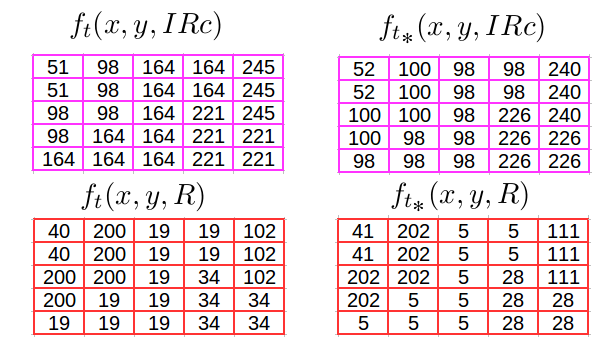
\includegraphics[width=0.8	\textwidth]{./Figures/cap4/ejemplo_entrada.png}
	\caption{Bandas de im\'agenes satelitales utilizados como entrada.}
	\label{fig:ejemplo_1}
\end{figure}
El proceso de iteraci\'on empieza normalizando radiom\'etricamente las bandas de $ f_{t_{*}} $ de manera a buscar la semejanza con las bandas de $ f_{t} $. La normalizaci\'on es realizado mediante la ecuaci\'on \ref{ec:normalizacion} habiendo calculado los par\'ametros estad\'isticos (Algoritmo \ref{alg:parametros}) en base a una mascara de cambio $ MC $, donde inicialmente sus niveles digitales valen $ 1 $. La Figura \ref{fig:ejemplo_2} nos muestra todos los procedimientos realizados en la primera iteraci\'on. 

\begin{figure}[H]
	\centering
	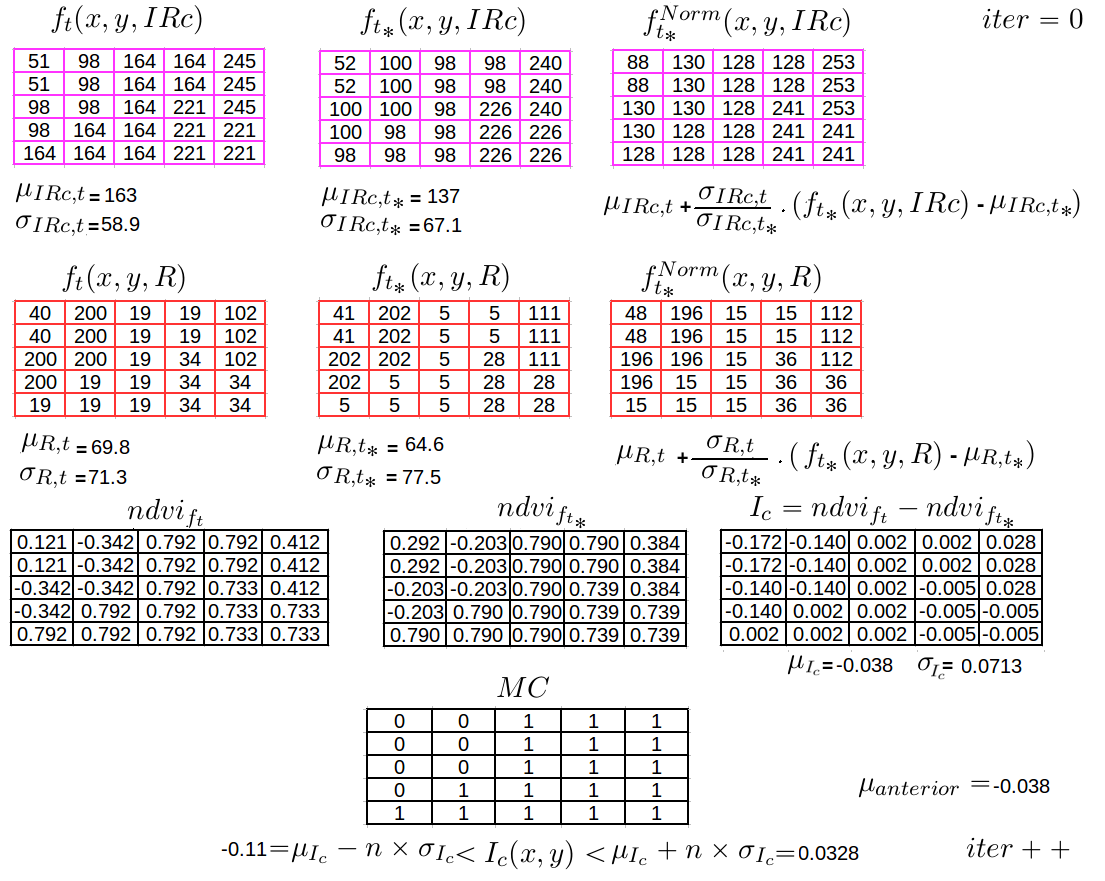
\includegraphics[width=1.0	\textwidth]{./Figures/cap4/ejemplo_iteracion_1.png}
	\caption{Primera iteraci\'on en el proceso de detecci\'on de cambio.}
	\label{fig:ejemplo_2}
\end{figure}
En la segunda iteraci\'on la mascara de cambio $ MC $ es tenido en cuenta para realizar el c\'alculo de los par\'ametros estad\'isticos solo sobre los pixeles que no sufrieron cambio ($ MC(x,y)=1 $). La Figura \ref{fig:ejemplo_3} nos muestra la segunda iteraci\'on, 
\begin{figure}[H]
	\centering
	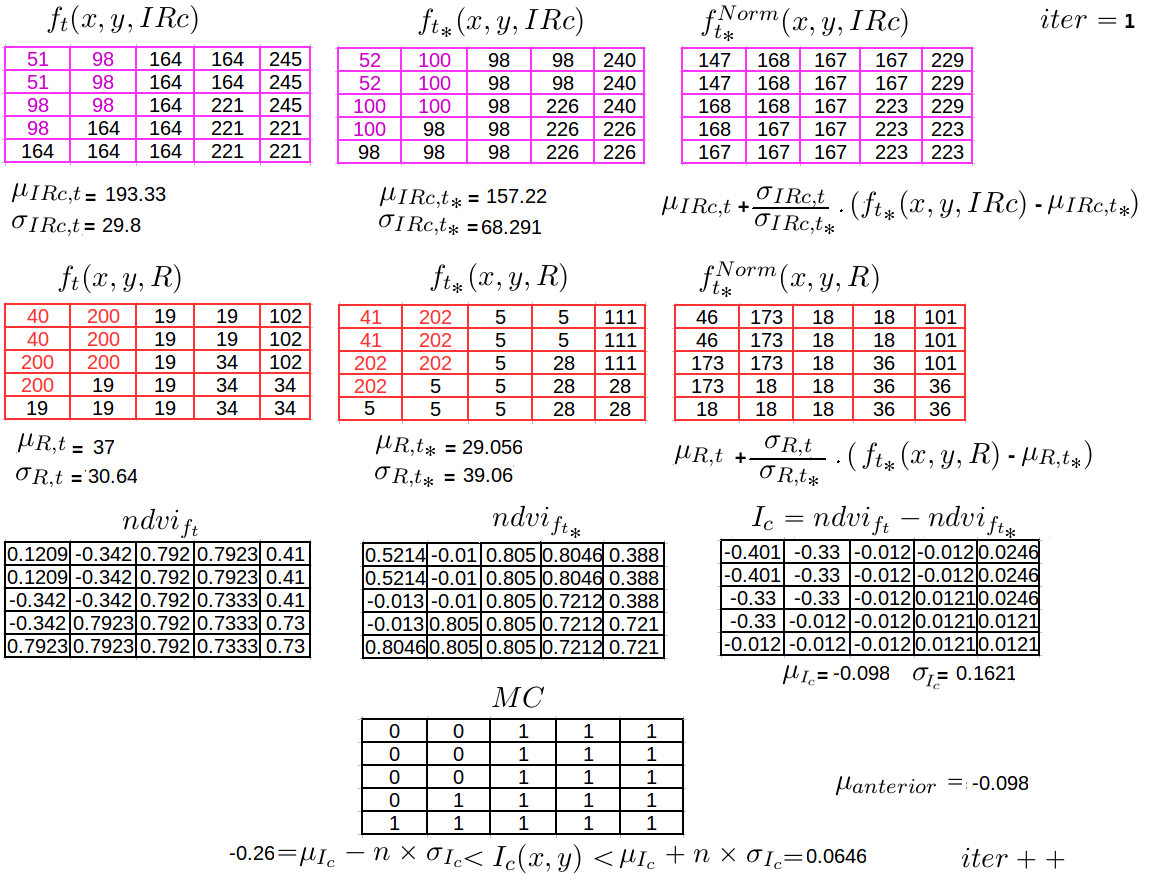
\includegraphics[width=1.0	\textwidth]{./Figures/cap4/ejemplo_iteracion_2.png}
	\caption{Segunda iteraci\'on en el proceso de detecci\'on de cambio.}
	\label{fig:ejemplo_3}
\end{figure}
En la Figura \ref{fig:ejemplo_4} podemos observar la siguiente iteraci\'on, donde la diferencia entre la media anterior $ \mu_{anterior} $ y la media de $ I_{c} $ actual ($ \mu_{I_{c}} $) cumple con la ecuaci\'on \ref{ec:continuar} para un $\epsilon=0 $, finalizando as\'i la iteraci\'on en la detecci\'on de cambio.
\begin{figure}[H]
	\centering
	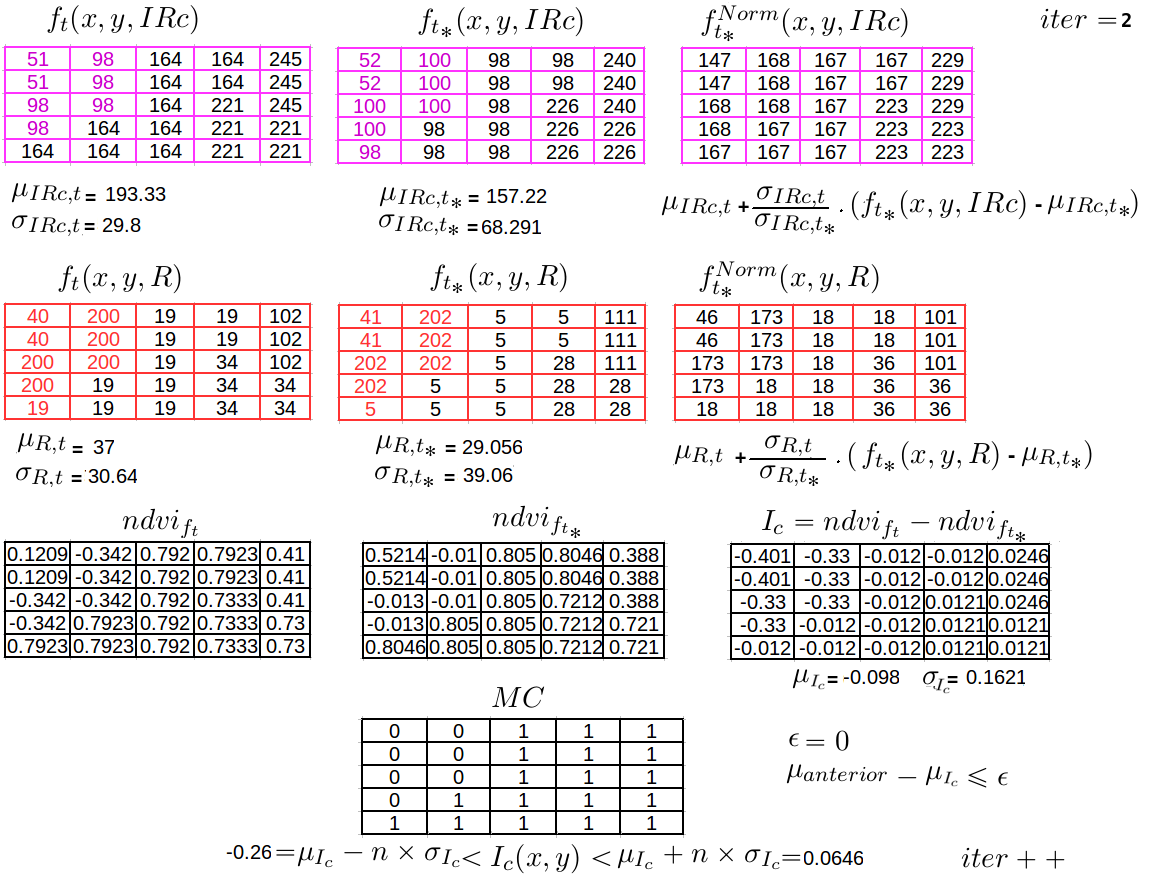
\includegraphics[width=1.0	\textwidth]{./Figures/cap4/ejemplo_iteracion_3.png}
	\caption{\'Ultima iteraci\'on en el proceso de detecci\'on de cambio.}
	\label{fig:ejemplo_4}
\end{figure}
La Figura \ref{fig:ejemplo_5} nos muestra como es obtenida la mascara de vegetaci\'on $ MV $ en en funci\'on a $ ndvi_{f_{t}} $ y $ ndvi_{f_{t_{*}}} $
\begin{figure}[H]
	\centering
	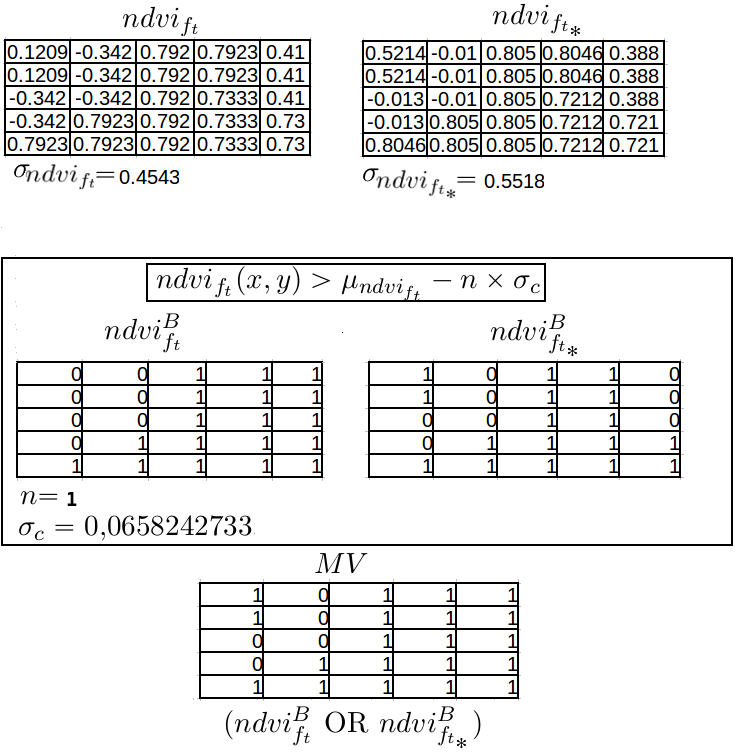
\includegraphics[width=0.8	\textwidth]{./Figures/cap4/ejemplo_ndvi.png}
	\caption{Determinaci\'on de la m\'ascara de vegetaci\'on $ MV $.}
	\label{fig:ejemplo_5}
\end{figure}
La Figura \ref{fig:ejemplo_6} podemos observar la forma en que es calculado la m\'ascara de perdida forestal y su cuantificaci\'on. En la figura se resalta en un cuadro rojo el resultado esperado por la metodología. 
\begin{figure}[H]
	\centering
	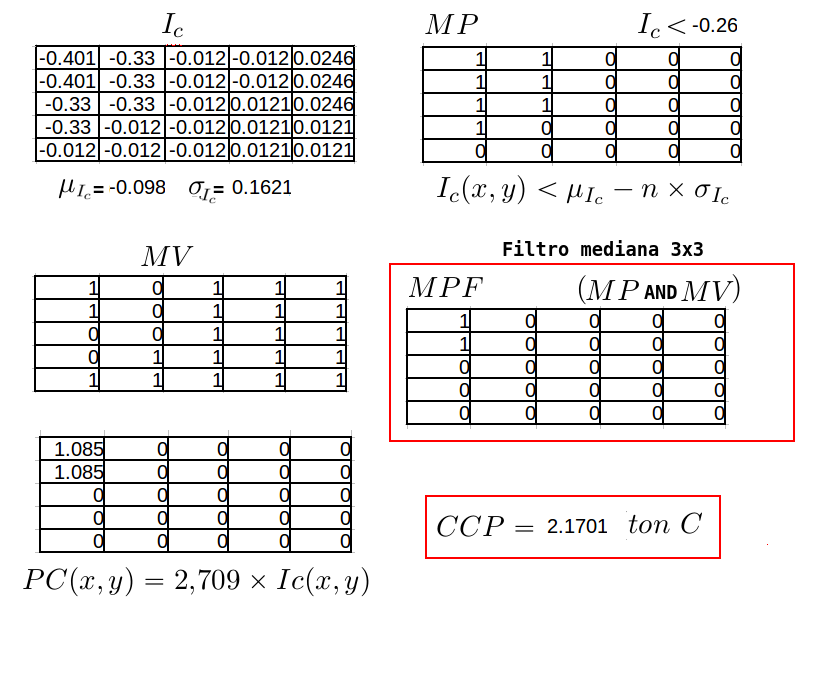
\includegraphics[width=0.8	\textwidth]{./Figures/cap4/ejemplo_resultado.png}
	\caption{Mascara de cambio forestal y cuantificaci\'on de perdida de carbono forestal.}
	\label{fig:ejemplo_6}
\end{figure}
\section{Resumen}
En este capitulo se describen los materiales y los tres procedimientos generales que componen la metodolog\'ia propuesta. La im\'agenes infrarroja cercana y roja de las dos fechas inicialmente deben pasar por un proceso de correcci\'on de errores del sensor y de ubicaci\'on geogr\'afica para realizar el an\'alisis multitemporal en la detecci\'on de cambio forestal. Una vez detectado la perdida forestal entre las fechas del proceso de detecci\'on de cambio, se realiza la estimaci\'on de carbono en base a una ecuaci\'on de regresi\'on hallado por un estudio previo. El resultado consiste en un mapa de perdida forestal junto a la cuantificaci\'on en toneladas de carbono perdidos.
\newpage{\ } 
\thispagestyle{empty} 

\chapter{Pruebas experimentales}
\lhead{Cap\'itulo 5. \emph{Pruebas experimentales}} % This is for the header on each page - perhaps a shortened title
En este capítulo se menciona las m\'etricas de evaluaci\'on utilizadas para medir el desempe\~{n}o de la metodolog\'ia propuesta. Por otro lado, se detallan los experimentos realizados y los resultados de la metodolog\'ia propuesta, seguidamente se esboza la comparaci\'on y la posterior discusi\'on de los mismos.

\section{Caso de estudio}
Filadelfia es una ciudad de Paraguay, del departamento de Boquer\'on, del Chaco paraguayo(lat-long $22^{o}20^{,}00^{,,} S - 60^{o}01^{,} 00^{,,} O$ ) con una superficie de 13.879 $ km^{2} $. Fue elevada a nivel de distrito en 2006. Su poblaci\'on la constituyen principalmente colonos menonitas. Fundada junto a otras localidades menonitas a finales de la d'ecada de 1920, ha desarrollado una cultura espec\'ifica, transmitida a lo largo de los siglos a trav\'es de la religi\'on, y una infraestructura productiva que le aporta a sus residentes alto poder de compra. Estas comunidades menonitas trabajan con modernas t\'ecnicas de producci\'on agropecuaria, fabricaci\'on de productos l\'acteos y procesamiento de s\'esamo y man\'i. Pueden ser ubicadas dentro de las imagenes landsat con path-Row 228-76 y en las VCF con c\'odigo KJ1920.\\~\\
Se opto por esta localizaci\'on debido a que ademas de estar ubicada en el Chaco Paraguayo posee un crecimiento demogr\'afico en la que las actividades agr\'icolas y ganaderas son variantes, proporcionando un ambiente ideal para las distintas pruebas y validaciones necesarias.\\~\\

\section{Métricas de evaluación}
Para realizar el control de calidad, algunos se basan en el concepto de matriz de confusi\'on, que establece una relaci\'on entre los resultados obtenidos en el proceso de asignaci\'on y la informaci\'on verdad terreno $ (VT) $ disponible para la zona de estudio. La diagonal principal representa el n\'umero de celdas correctamente catalogadas $ (T) $ , y la diagonal transpuesta, las incorrectamente catalogadas $ (F) $ . El uso de esta matriz presenta como mayor desventaja que est\'a condicionada a la veracidad y exactitud de la referencia utilizada como $ VT $.

\begin{table}[H]
	\centering
\begin{tabular}{|
		>{\columncolor[HTML]{EFEFEF}}l |l|l|l|}
	\hline
	\textbf{Categorias}             & \cellcolor[HTML]{EFEFEF}\textbf{Perdida (VT)} & \cellcolor[HTML]{EFEFEF}\textbf{No Perdida (VT)} & \cellcolor[HTML]{EFEFEF}\textbf{Total (VT)} \\ \hline
	\textbf{Perdida (Algoritmo)}    & TP                                            & FP                                               & P                                           \\ \hline
	\textbf{No Perdida (Algoritmo)} & FN                                            & TN                                               & N                                           \\ \hline
	\textbf{Total (Algoritmo)}      & P'                                            & N'                                               & Total                                       \\ \hline
\end{tabular}
		\caption{Matriz de Confusi\'on}
		\label{t:matrizConfusion}
\end{table}

Esta matriz de confusi\'on, permite extraer distintos par\'ametros que eval\'uen la calidad del resultado obtenido en un proceso de detecci\'on de cambios utilizando t\'ecnicas de teledetecci\'on. A continuación se explican los dos par\'ametros m\'as utilizados para este propósito: el porcentaje de precisi\'on global y el coeficiente Kappa. Estas medidas de la precisi\'on se han utilizado para evaluar diferentes m\'etodos de detecci\'on de cambio\cite{foody2002status}.

\subsection{Porcentaje de precisi\'on global}\label{sec:pg}
El porcentaje de precisi\'on global (Global Acurrancy, GA) se define como la suma del n\'umero de celdas clasificadas correctamente y dividiendo por el n\'umero total de celdas que componen el \'area de referencia que representa la verdad terreno. Foody \cite{foody2002status} considera \'optimo cualquier resultado a partir de un 85 de precisión global. Seguidamente se muestra la expresi\'on matem\'atica de la precisi\'on global.
		\begin{equation}
		GA = \frac{TP+TN}{T+F}\cdot100
		\end{equation}
\subsection{Coeficiente Kappa}\label{sec:kappa}
El coeficiente Kappa es otro indicador utilizado frecuentemente en un proceso de teledetecci\'on, en la fase correspondiente al control de calidad de los resultados \cite{chuvieco1998factor}. Este \'indice es una medida de la correspondencia entre los resultados de la detecci\'on de cambios y los datos verdad-terreno tomados como referencia, en relaci\'on a la exactitud de una variable aleatoria, en otras palabras, es una medida estad\'istica que ajusta el efecto del azar en la proporci\'on de la concordancia observada para elementos cualitativos (variables categ\'oricas).\\~\\
Seg\'un se indica en Jensen \cite{jensen1981urban}, en detecci\'on de cambios en zonas urbanas es m\'as apropiado utilizar el coeficiente Kappa, puesto que hace uso de toda la matriz de error.

		\begin{equation}
		KAPPA=\dfrac{Total.(TP+TN)-(P.P'+N.N')}{Total^{2}.(P.P'+N.N')}\cdot100
		\end{equation}
		
		% Please add the following required packages to your document preamble:
		% \usepackage[table,xcdraw]{xcolor}
		% If you use beamer only pass "xcolor=table" option, i.e. \documentclass[xcolor=table]{beamer}
		\begin{table}[H]
			\centering
			\begin{tabular}{|l|l|}
				\hline
				\rowcolor[HTML]{EFEFEF} 
				\textbf{Coeficiente Kappa} & \textbf{Fuerza de la concordancia} \\ \hline
				0,00                       & Pobre                              \\ \hline
				0,01-0,20                  & Leve                               \\ \hline
				0,21-0,40                  & Aceptable                          \\ \hline
				0,41-0,60                  & Moderada                           \\ \hline
				0,61-80                    & Considerable                       \\ \hline
				0,81-1,00                  & Casi perfecta                      \\ \hline
			\end{tabular}
						\caption{Valoración del coeficiente kappa\cite{landis1977measurement}.}
						\label{t:kappaTable}
		\end{table}
		


\section{Pruebas y resultados experimentales}
En esta secci\'on se describir\'an las diferentes pruebas desarrolladas para la determinaci\'on de constantes establecidas dentro de los proceso metodol\'ogicos. Igualmente se exponen los resultados obtenidos por la metodolog\'ia empleado en el estado del arte, de manera a evaluar los datos de salida a trav\'es de m\'etricas de evaluaci\'on.
\subsection{Umbral de Vegetaci\'on} 
En la metodolog\'ia hemos hablado y utilizado una variable estad\'istica\ref{sec:uvegetacion} hallada por un an\'alisis previo del comportamiento espectral que presenta la cobertura vegetal. Dicha variable corresponde a la desviaci\'on.\\~\\
Partiendo del las im\'agenes VCF \ref{sec:vcf} junto con las im\'agenes Landsat \ref{sec:landsat}, se elaboro un cruzamiento de datos. En las im\'agenes VCF, los p\'ixeles representan proporciones de vegetaci\'on existente en un espacio geogr\'afico, mientras que las im\'agenes Landsat nos permite calcular NDVI. Se procedi\'o a la obtenci\'on y calculo del NDVI en diferentes tiempos (1986,1990,2000) teniendo como referencia la fecha de la imagen VCF. Existe una colecci\'on disponible de im\'agenes VCF, del a\~{n}o 2000 hasta el 2010, en la que se tomo el a\~{n}o 2000 como referencia, por observar mayor porcentaje de cobertura vegetal que las dem\'as. Una vez obtenidos los NDVI de cada fecha, se elaboro mascaras de la imagen VCF, en la que representaba existencia de vegetaci\'on para cada rango de porcentaje. Los rangos var\'ian de 0-10, 0-20, 0-30, 0-40 y 0-50, no se analizaron en el rango completo debido a lo no existencia de p\'ixeles con los valores.
\begin{figure}[H]
	\centering
	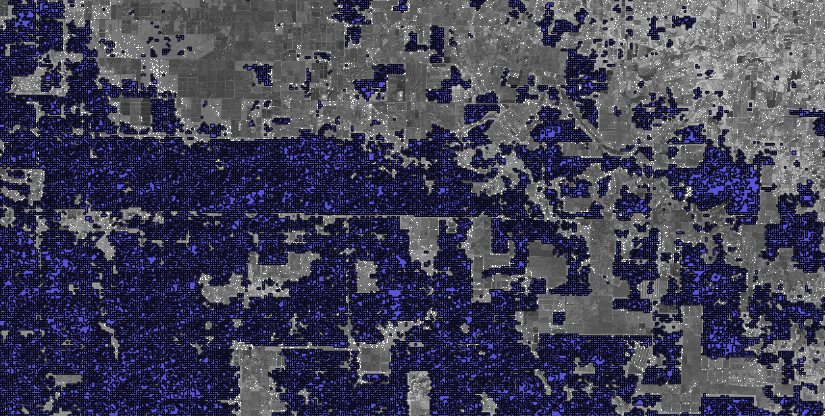
\includegraphics[width=0.8	\textwidth]{./Figures/cap5/mascaraVCF.png}
	\caption{Mascara VCF de 0-30\% sobre NDVI a\~{n}o 2000}
	\label{fig:mascVCf}
\end{figure}
Posteriormente se extrajeron 2000 puntos aleatorios, para muestreo, de la mascara VCF, donde estaran los valores de NDVI..
\begin{figure}[H]
	\centering
	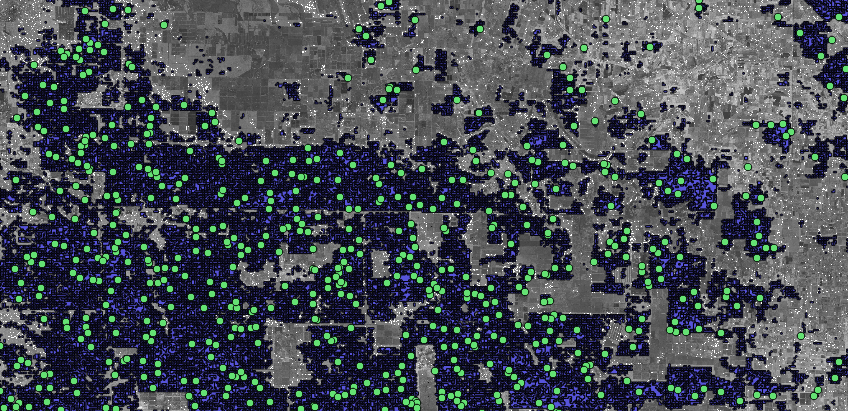
\includegraphics[width=0.8	\textwidth]{./Figures/cap5/vcfAleatorio.png}
	\caption{Puntos aleatorios dentro de la mascara VCF.}
	\label{fig:aleatorioVCf}
\end{figure}
El procedimiento se repite para cada mascara en los distintos rangos. En total se obtiene 5 grupos por cada a\~{n}o estudiado con estad\'isticas ilustrada en la tabla \ref{t:vcfNdvi}.

% Please add the following required packages to your document preamble:
% \usepackage[table,xcdraw]{xcolor}
% If you use beamer only pass "xcolor=table" option, i.e. \documentclass[xcolor=table]{beamer}
\begin{table}[H]
	\centering
	\begin{tabular}{|l|l|l|}
		\hline
		\rowcolor[HTML]{EFEFEF} 
		\multicolumn{3}{|c|}{\cellcolor[HTML]{EFEFEF}\textbf{A\~{n}o 1986}}        \\ \hline
		\rowcolor[HTML]{EFEFEF} 
		\textbf{VCF (\%)} & \textbf{NDVI (Media)} & \textbf{NDVI (Desviaci\'on)} \\ \hline
		50                & 0.356701              & 0.047891                   \\ \hline
		40                & 0.344022              & 0.0507296                  \\ \hline
		30                & 0.337696              & 0.061581                   \\ \hline
		20                & 0.339586              & 0.0632055                  \\ \hline
		10                & 0.335528              & 0.0727573                  \\ \hline
		\rowcolor[HTML]{EFEFEF} 
		\multicolumn{3}{|c|}{\cellcolor[HTML]{EFEFEF}\textbf{A\~{n}o 1990}}        \\ \hline
		\rowcolor[HTML]{EFEFEF} 
		\textbf{VCF (\%)} & \textbf{NDVI (Media)} & \textbf{NDVI (Desviaci\'on)} \\ \hline
		50                & 0.278804              & 0.0631834                  \\ \hline
		40                & 0.264651              & 0.0679451                  \\ \hline
		30                & 0.254145              & 0.0742348                  \\ \hline
		20                & 0.252186              & 0.0759032                  \\ \hline
		10                & 0.251421              & 0.0796667                  \\ \hline
		\rowcolor[HTML]{EFEFEF} 
		\multicolumn{3}{|c|}{\cellcolor[HTML]{EFEFEF}\textbf{A\~{n}o 1990}}        \\ \hline
		\rowcolor[HTML]{EFEFEF} 
		\textbf{VCF (\%)} & \textbf{NDVI (Media)} & \textbf{NDVI (Desviaci\'on)} \\ \hline
		50                & 0.0202133             & 0.0572825                  \\ \hline
		40                & 0.0104289             & 0.0608757                  \\ \hline
		30                & -0.00337075           & 0.066776                   \\ \hline
		20                & -0.00663188           & 0.0695777                  \\ \hline
		10                & -0.0103891            & 0.0757546                  \\ \hline
	\end{tabular}
		\caption{Media y desviaci\'on del muestreo realizado.}
		\label{t:vcfNdvi}
\end{table}

La tabla nos muestra claramente, que la media del NDVI es diferente para cada a\~{n}o, independientemente del porcentaje de vegetaci\'on evaluado. En este caso, no es conveniente tomar la media dentro de un patrón de comportamiento, con el fin de discriminar la vegetaci\'on. Por otro lado, las desviaciones presentan peque\~{n}as diferencias no considerables, lo cual es debido, a que el \'area foliar (hojas) en la vegetaci\'on posee diferente vigor en cada estaci\'on o condici\'on clim\'atica, al momento de ser capturado su reflectividad por sensores del sat\'elite.\\~\\
De esta manera se realiza un promedio entre todas las desviaciones, quedando como valor constante en la umbralizaci\'on de vegetaci\'on \ref{sec:uvegetacion}$ \sigma_{ndvi} = 0.0658242733 $.
\subsection{Estimaci\'on de p\'erdida de carbono forestal}
Gracias al Mapa Global de Carbono \ref{sec:saatchiMapa} es posible analizar la relaci\'on que posee con los indices de vegetaci\'on. El mapa corresponde a fechas cercanas al a\~{n}o 2000, por lo que para el estudio, se obtuvieron im\'agenes Landsat del a\~{n}o 2003 para el calculo de NDVI. Posteriormente se generaron 240 puntos aleatorios dentro \'areas que correspond\'ian a vegetaci\'on.
\begin{figure}[H]
	\centering
	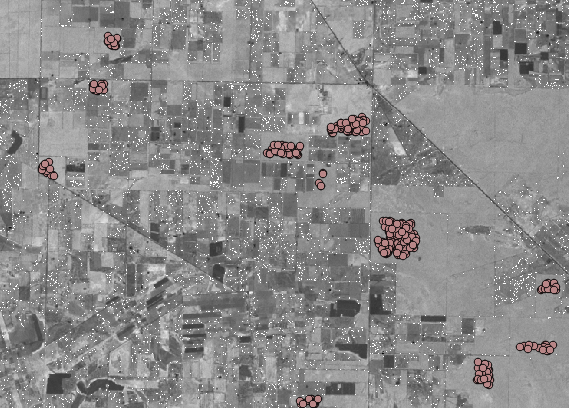
\includegraphics[width=0.8	\textwidth]{./Figures/cap5/carbNdvi.png}
	\caption{Puntos aleatorios.}
	\label{fig:aleatorioCrb}
\end{figure}
Estos puntos fueron generados para interceptar en ellos, los NDVI y ton C/ha en el espacio geográfico. De esa manera nos permiti\'o realizar un an\'alisis de regresi\'on. Inicialmente se hallo una ecuaci\'on lineal, donde el coeficiente de determinaci\'on fue moderado ($ r^{2}=0.509125 $).
\begin{figure}[H]
	\centering
	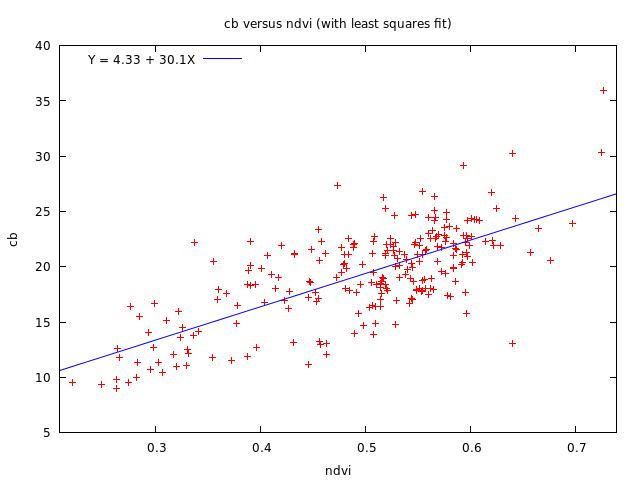
\includegraphics[width=0.8	\textwidth]{./Figures/cap4/ndviCarb.png}
	\caption{Regresi\'on Lineal. $ X=NDVI, Y=TonC/ha $}
	\label{fig:linealCar}
\end{figure}
En la misma forma se construyo una ecuaci\'on cuadr\'atica, pero el coeficiente de determinaci\'on era semejante al lineal $ r^{2}=0.509273 $.
\begin{figure}[H]
	\centering
	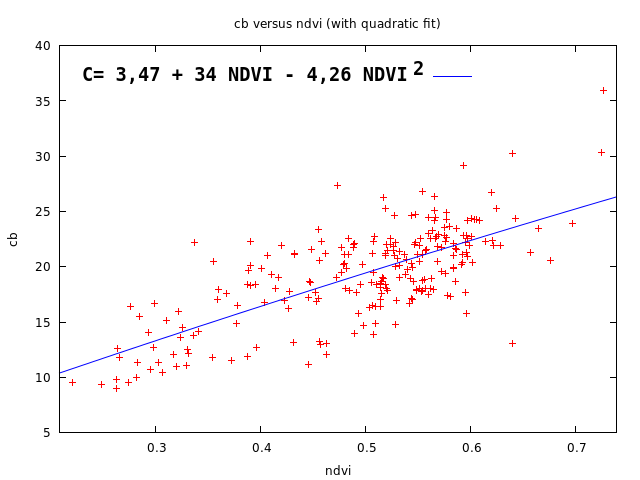
\includegraphics[width=0.8	\textwidth]{./Figures/cap4/ndvCarCuadratico.png}
	\caption{Regresi\'on cuadr\'atica. $ X=NDVI, Y=TonC/ha $}
	\label{fig:cuaCar}
\end{figure}
De esta manera, se opta por la ecuaci\'on lineal para el calculo de carbono en funci\'on al NDVI:
		\begin{equation}
		C=4,33+30,1 NDVI
		\end{equation} 
Siendo $ C $ toneladas de carbono por hect\'area.

\subsection{Prueba experimental} 
Con el prop\'osito de evaluar la calidad en la detecci\'on de cambio, se obtuvieron las im\'agenes que fueron utilizadas en la elaboraci\'on del Paraguay Forest Change Product \ref{sec:fcc}. Dichas im\'agenes corresponden a la fecha 1-26-1992	del sat\'elite Landsat-5 y 8-17-1999 del satelite Landsat-7, con path-row 228-76 del WRS-2 correspondiente al \'area del caso de estudio.\\~\\
Se delimitaron 3 tipos de \'areas, donde cada uno representa un sector las \'areas urbana, rural y h\'umeda. Esto es con el fin de evaluar la detecci\'on en diferentes condiciones o usos del suelo.
\begin{itemize}
	\item \textbf{\'Area Urbana:} zona de aglomeramiento y mayor densidad poblacional. Existe predominio  de actividades econ\'omicas no agropecuarias, sumado a la poblaci\'on total. 
	\item \textbf{\'Area Rural:} se caracteriza por la inmensidad de espacios verdes que la componen y que por esta razón est\'a destinada y es utilizada para la realizaci\'on de actividades agropecuarias y agro-industriales, entre otras.
	\item \textbf{\'Area H\'umeda:}	zona de tierras, generalmente planas, cuya superficie se inunda de manera permanente o intermitente-mente.
\end{itemize}
\begin{figure}[H]
	\centering
	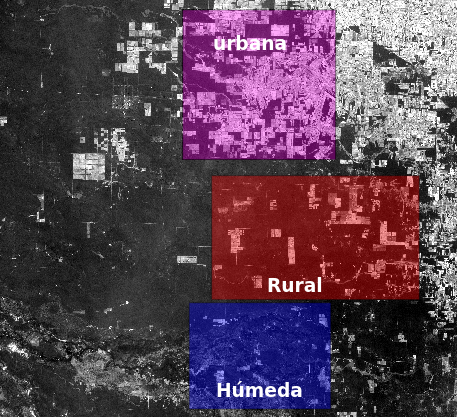
\includegraphics[width=0.8	\textwidth]{./Figures/cap5/zonas.png}
	\caption{Sectores de estudio.}
	\label{fig:zonasEva}
\end{figure}
\begin{table}[H]
	\centering
	\begin{tabular}{|l|l|l|l|l|l|l|}
		\hline
		\rowcolor[HTML]{EFEFEF} 
		\textbf{Sector} & \textbf{xMin} & \textbf{yMin} & \textbf{xMax} & \textbf{yMax} & \textbf{Has.} & \textbf{Km.} \\ \hline
		Urbano          & 748797.48     & -2532113.76   & 799869.96     & -2482116.50 & 255348.41 & 202.13   \\ \hline
		Rural           & 758474.37     & -2578885.40   & 827825.42     & -2537489.81 & 287082.72 & 221.49  \\ \hline
		Húmedo          & 750947.90     & -2615442.54   & 798257.14     & -2579960.61 & 167862.32 & 165.58	  \\ \hline
	\end{tabular}
		\caption{Pol\'igono de las \'areas. Sistema de coordenadas UTM Zona 20 K. }
		\label{t:poligonos}
\end{table}
La metodolog\'ia fue implementada como un complemento al Quantum GIS\ref{sec:quantum}, de manera a poder realizar las pruebas. 
\begin{figure}[H]
	\centering
	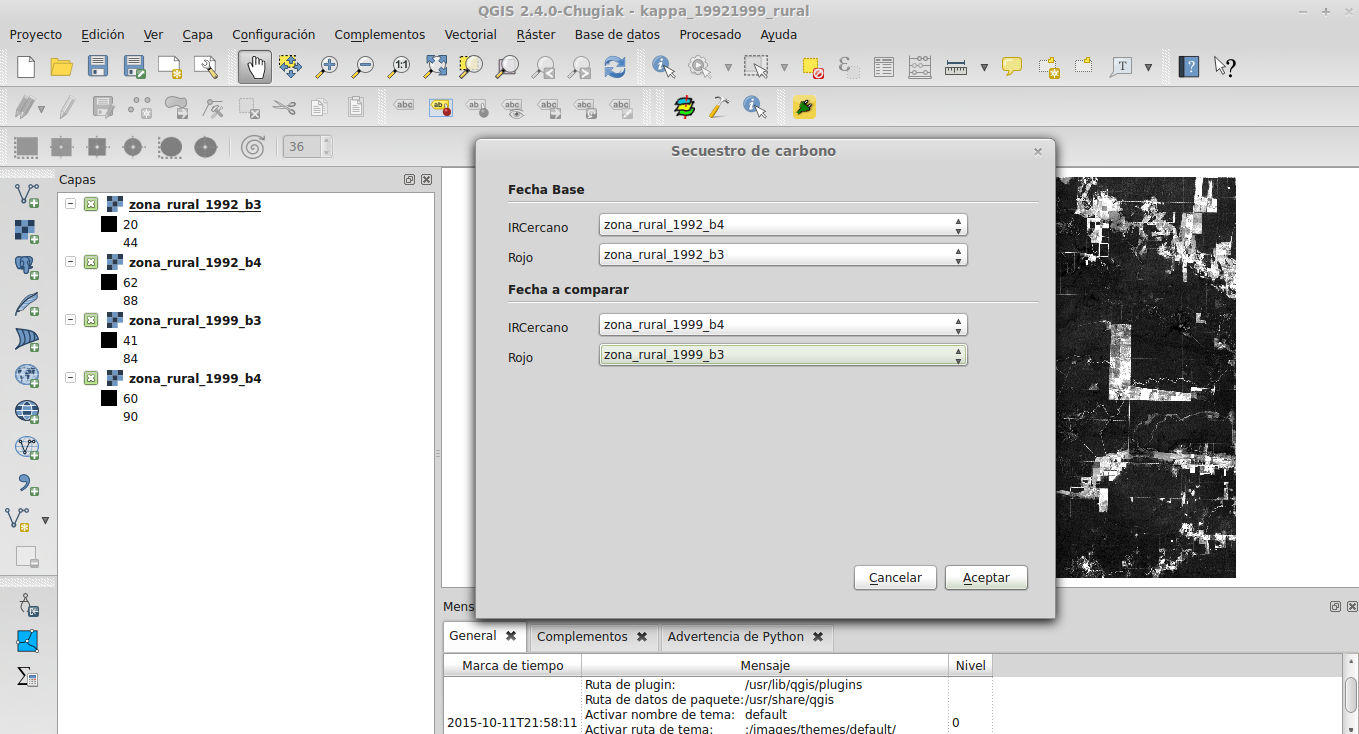
\includegraphics[width=0.8	\textwidth]{./Figures/cap5/qgisCarbono.png}
	\caption{Complemento Quantum GIS.}
	\label{fig:qgisC}
\end{figure}
El proceso de correcci\'on de las im\'agenes satelitales \ref{sec:coorImsat}, debido a que obtuvieron los productos L1T del USGS \ref{sec:landsat}, no fueron implementados por ya poseer el pre-procesamiento de correcci\'on geom\'etrica y radiom\'etrica correspondiente. Esto es beneficioso al estudio en cuanto a costo, por que no es necesario el levantamiento de los puntos de control (GCP) en el terreno para la correcci\'on geom\'etrica espec\'ificamente. La interpolaci\'on espacial fue hecha por un polinomio cuadr\'atico y la radiom\'etrica por el m\'etodo de convoluci\'on cubica.
% Please add the following required packages to your document preamble:
% \usepackage[table,xcdraw]{xcolor}
% If you use beamer only pass "xcolor=table" option, i.e. \documentclass[xcolor=table]{beamer}
\begin{table}[H]
	\centering

	\begin{tabular}{|l|l|l|l|l|}
		\hline
		\rowcolor[HTML]{EFEFEF} 
		\textbf{Sat\'elite} & \textbf{Path-row} & \textbf{Fecha} & \textbf{RMSE} & \textbf{GCP} \\ \hline
		Landsat-5         & 228-76            & 1-26-199       & 4.302         & 108          \\ \hline
		Landsat-7         & 229-76            & 8-17-1999      & 4.066         & 199          \\ \hline
	\end{tabular}
		\caption{RMSE obtenido del meta-dato de cada imagen obtenida.}
		\label{t:rmse}
\end{table}

Se recortaron las bandas de las im\'agenes, infrarroja cercana y roja $ (B4,B3) $, para cada sector y fecha e introducidas como datos de entrada al complemento, ilustraci\'on \ref{fig:qgisC}. A continuaci\'on se muestran los resultados de cada sector con diferentes coeficientes de tolerancia, descripto en la secci\'on \ref{sec:discriminacion}, luego de pasar por el complemento:
\begin{figure}[H]
	\centering
	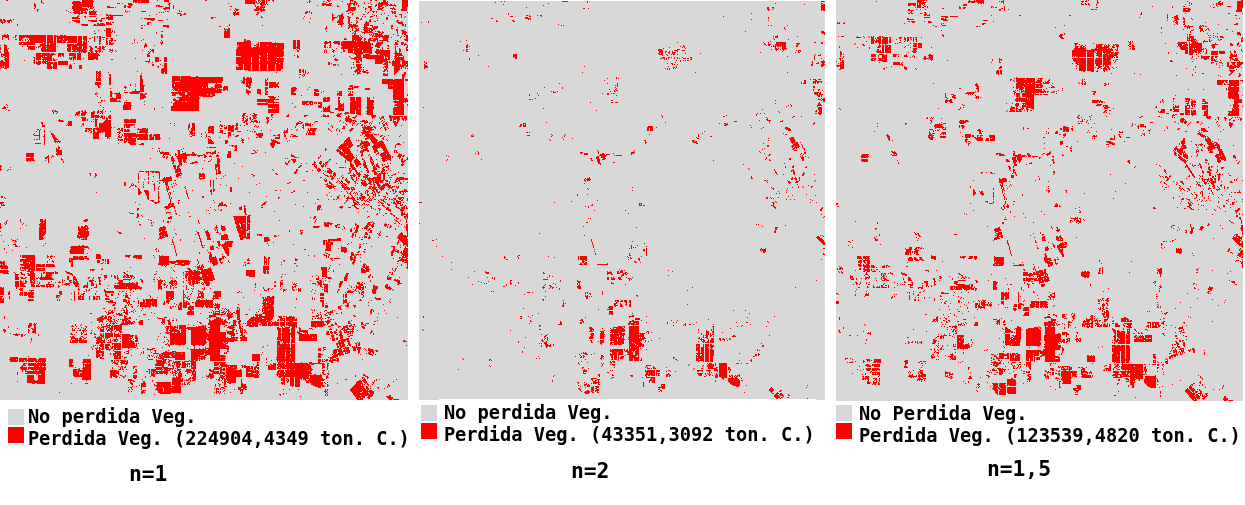
\includegraphics[width=0.8	\textwidth]{./Figures/cap5/res_zona_urbana.png}
	\caption{\'Area Urbana.}
	\label{fig:ubana}
\end{figure}
\begin{figure}[H]
	\centering
	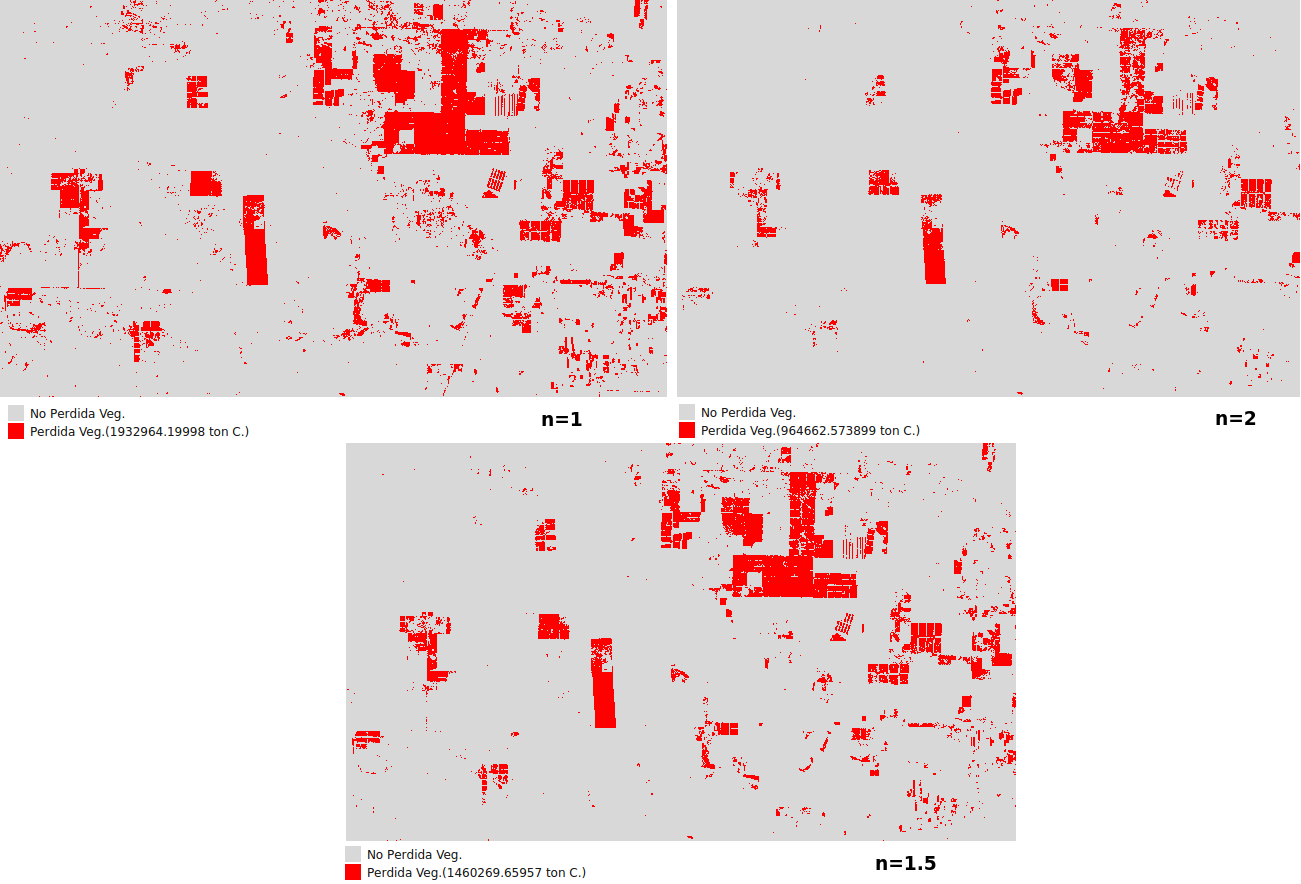
\includegraphics[width=0.8	\textwidth]{./Figures/cap5/res_zona_rural.png}
	\caption{\'Area Rural.}
	\label{fig:rural}
\end{figure}
\begin{figure}[H]
	\centering
	\includegraphics[width=0.8	\textwidth]{./Figures/cap5/res_zona_humeda.png}
	\caption{\'Area H\'umeda.}
	\label{fig:humeda}
\end{figure}

\subsection{Discusi\'on de resultados}
La evaluaci\'on de la calidad en la detecci\'on de perdida forestal fueron hechas con la comparaci\'on del Paraguay Forest Change Produc (PFCP) y los resultados obtenidos por cada sector y coeficiente de tolerancia $ (n) $. El indice kappa y la precision Global nos permitira saber la calidad en los resultados de detecci\'on de cambio.\\~\\
Previamente se realizo una re-clasificaci\'on en la imagen PFCP, ya que en ella refleja varios tipos de bosques y no bosques, por ello se procedi\'o a dejar solo aquellos pixeles que representan perdida de vegetaci\'on en cualquier de los tipos.
\begin{figure}[H]
	\centering
	\includegraphics[width=0.8	\textwidth]{./Figures/cap5/pcfp.png}
	\caption{Re-clasificaci\'on de la imagen PFCP. Perdida = 2, Otros=1}
	\label{fig:pfcp}
\end{figure}
Una vez generado la imagen de referencia para la evaluaci\'on, con ayuda de la aplicaci\'on GRASS GIS \ref{sec:grass} se obtuvo los siguientes resultados:
% Please add the following required packages to your document preamble:
% \usepackage[table,xcdraw]{xcolor}
% If you use beamer only pass "xcolor=table" option, i.e. \documentclass[xcolor=table]{beamer}
\begin{table}[H]
	\centering

	\begin{tabular}{|l|l|l|}
		\hline
		\rowcolor[HTML]{EFEFEF} 
		\multicolumn{3}{|l|}{\cellcolor[HTML]{EFEFEF}\textbf{N=1}}   \\ \hline
		\rowcolor[HTML]{EFEFEF} 
		\textbf{\'Area}  & \textbf{Kappa}  & \textbf{Precisi\'on Global} \\ \hline
		Urbano         & 0.476389        & 84.257452                 \\ \hline
		Rural          & 0.65782         & 93.82121                  \\ \hline
		H\'umeda         & 0.301541        & 90.624794                 \\ \hline
		\rowcolor[HTML]{EFEFEF} 
		\multicolumn{3}{|l|}{\cellcolor[HTML]{EFEFEF}\textbf{N=1.5}} \\ \hline
		\rowcolor[HTML]{EFEFEF} 
		\textbf{\'Area}  & \textbf{Kappa}  & \textbf{Precisi\'on Global} \\ \hline
		Urbano         & 0.315273        & 83.514875                 \\ \hline
		Rural          & 0.671753        & 94.899171                 \\ \hline
		H\'umeda         & 0.425555        & 96.693648                 \\ \hline
		\rowcolor[HTML]{EFEFEF} 
		\multicolumn{3}{|l|}{\cellcolor[HTML]{EFEFEF}\textbf{N=2}}   \\ \hline
		\rowcolor[HTML]{EFEFEF} 
		\textbf{\'Area}  & \textbf{Kappa}  & \textbf{Precisi\'on Global} \\ \hline
		Urbano         & 0.09368         & 81.642457                 \\ \hline
		Rural          & 0.570687        & 94.33648                  \\ \hline
		H\'umeda         & 0.425555        & 96.693648                 \\ \hline
	\end{tabular}
		\caption{Coeficiente Kappa y precisi\'on Global obtenidos.}
		\label{t:kappaGa}
\end{table}

En la figura \ref{fig:kappaGrafico}, podemos observar que los coeficientes kappas en todos los $ n  $ son mejores para zonas rurales, variando en resultados moderados y considerables. Seguido por zonas h\'umedas, donde $ n=1 $ se obtienen resultados aceptables a diferencia de las dem\'as que son moderadas. Por ultimo las zonas urbanos son las que presentan gran variaci\'on entre los coeficientes hallados para el, debiendo implementar tolerancia baja $(n=1)$, al modelo de detecci\'on, para obtener resultados moderados. Los coeficientes son interpretados seg\'un la tabla \ref{t:kappaTable}.
\begin{figure}[H]
	\centering
	\includegraphics[width=0.8	\textwidth]{./Figures/cap5/kappaGrafico.png}
	\caption{Coeficiente Kappa por cada \'Area y tolerancia.}
	\label{fig:kappaGrafico}
\end{figure}


La precisi\'on global, seg\'un la ilustraci\'on \ref{fig:gaGrafico}, nos dice que el mejor resultado fue en la zona h\'umeda $ (n=2) $ bajando el porcentaje para los dem\'as tolerancias. Pero en zonas rurales obtenemos porcentajes parejos y elevados para cualquier $ n $. Tanto para zonas h\'umedas y rurales seg\'un Jensen \cite{jensen1981urban} son \'optimos por sobrepasar el 85\%. Las zonas urbanas se encuentran entre 81\% - 85\% proximos al umbral, lo que los deja sin ning\'un resultado satisfactorio.
\begin{figure}[H]
	\centering
	\includegraphics[width=0.8	\textwidth]{./Figures/cap5/gaGrafico.png}
	\caption{GA por cada \'Area y tolerancia.}
	\label{fig:gaGrafico}
\end{figure}

\subsection{Dificultades encontradas} 
Unas de las principales dificultades encontradas fueron en el proceso de correcci\'on geom\'etrica, debido a que es necesario ir al terreno para el levantamiento de puntos de control, sino se utilizan las im\'agenes Landsat prove\'idas por USGS \ref{sec:landsat}. Otro punto considerable a lo que se refiere a dificultad, es que las im\'agenes Landsat presentan un porcentaje de nubosidad, por lo que requerir\'a un pre-procesamiento que permita su utilizaci\'on en el an\'alisis.\\~\\

Habiendo evaluado los resultados en base a los objetivos propuestos, en el siguiente y \'ultimo cap\'itulo se exponen las conclusiones de este trabajo  y finalmente trabajos futuros que puedan dar continuidad a este trabajo final de grado.
\newpage{\ } 
\thispagestyle{empty} 

\chapter{Conclusiones y trabajos futuros}
\lhead{Capítulo 6. \emph{Conclusiones y trabajos futuros}}
%\lhead{Capítulo 6. \emph{Conclusiones y trabajos y futuros}} % This is for the header on each page - perhaps a shortened title
En base a los resultados obtenidos en la estimaci\'on de perdida de carbono en nuestra \'area de estudio, este cap\'itulo nos presenta las conclusiones y recomendaciones para investigaciones futuras derivadas del trabajo:
\section{Conclusiones}

\begin{itemize}
\item Una vez evaluado las diferentes zonas de nuestro caso de estudio, podemos darnos cuenta que la metodolog\'ia propuesta posee una mejor respuesta, respecto a la calidad, en \'areas rurales. Esto es debido a que el Coeficiente kappa o los indices de acuerdo var\'ian entre 0.57-0.67 y su precisi\'on global sobrepasan el umbral optimo de 85\%, para cada coeficiente de tolerancia $ n $. Por lo que se considera satisfactorio la metodolog\'ia propuesta, ya que la perdida de carbono es un fen\'omeno frecuente en \'areas con vegetaci\'on predominante.

\item Para zonas donde la vegetaci\'on no predomina, esta metodolog\'ia podr\'ia no resultar suficientemente conveniente. Las pruebas experimentales hechas en zonas urbanas, la precisi\'on global y el coeficiente kappa no son \'optimos por el cual se llega a esa interpretaci\'on.

\item En \'areas cercanas a r\'ios o sujetas a inundaci\'on, se observaron resultados aceptables para  estudios con tolerancias medias y altas en la detecci\'on de perdida forestal. Por lo que el monitoreo en estos tipos de zonas con la metodolog\'ia propuesta podr\'ia ser aun de gran utilidad, ya que la presencia de agua en la vegetaci\'on modifica la respuesta espectral, dificultando su clasificaci\'on como cobertura vegetal.

\item Mediante los an\'alisis estad\'isticos empleados tanto para la determinaci\'on de umbrales vegetaci\'on/no vegetaci\'on como en el hallazgo de ecuaciones de transformaci\'on a carbono, nos indica que empleando extracciones de indices vegetales y variables estad\'isticas es posible generar metodolog\'ias no complejas destinadas al monitorio ambiental. Esta sencillez nos libera de necesarias supervisiones y entrenamientos normalmente empleadas en teledetecci\'on.

\item El mapa global de carbono \cite{saatchi2011benchmark} constituyo un factor importante para la automatizaci\'on, al permitir determinar una ecuaci\'on que transforme el indice vegetal a carbono. De no existir, hubiese sido necesario aplicar previos muestreos forestales en el terreno.

\item La correcci\'on geom\'etrica implica procesos que engloba visitas al terreno para levantamientos de puntos de control requeridas en las interpolaciones. Gracias a la utilizaci\'on de im\'agenes Landsat L1T prove\'idas por la USGS, no fue necesario sumar ese costo a la metodolog\'ia, automatizando-la por no haber necesidad de realizar dicho procedimiento.

\end{itemize}

La idea al elegir como caso de estudio parte del chaco paraguayo, es la de actuar de impulsora en la generaci\'on de herramientas para el monitoreo ambiental, donde con el empleo de procesamientos digital de im\'agenes satelitales que conlleven t\'ecnicas computacionalmente sencillas y autom\'aticas podamos identificar alertas referentes a perdida en el contenido de carbono forestal. De manera que una vez detectado, a trav\'es de las estimaciones, se puedan generar pol\'iticas de acci\'on o prevenci\'on contra los da\~{n}os posibles al ambiente. El chaco paraguayo es una regi\'on muy afectada actualmente por la degradaci\'on y de-forestaci\'on en los bosques, donde la falta de recursos y el costo  elevado en el monitoreo dificulta las intervenciones a tiempo, constituyendo un caso ideal e impulsora para la aplicaci\'on de metodolog\'ias como la propuestas en esta investigaci\'on.



\section{Trabajos futuros}
Se pretende que la metodolog\'ia propuesta siga mejorando en t\'erminos de pre-procesamiento de las im\'agenes satelitales, ante factores que influyan en el momento de captura de los datos hechas por sensores remotos como tambi\'en en t\'ecnicas que permita mejora la detecci\'on de cambio forestal, por lo que mencionamos como trabajos futuros:
\begin{itemize}
\item Proponer t\'ecnicas que permitan detectar y eliminar nubosidad en las imagen satelitales.
\item Mejorar la precisi\'on global y el coeficiente kappa para zonas urbanas.
\item Dise\~{n}ar mejores t\'ecnicas que clasifique cobertura vegetal mediante la extracci\'on de indices en todas las bandas.
\item Adaptar la metodolog\'ia, de manera a que permita recibir im\'agenes satelitales con diferentes resoluciones radiom\'etricas.

\end{itemize}

\newpage{\ } 
\thispagestyle{empty} 

%----------------------------------------------------------------------------------------
%	BIBLIOGRAPHY
%----------------------------------------------------------------------------------------

\lhead{\emph{Bibliografía}} % Change the page header to say "Bibliography"
%\bibliographystyle{apacite}
%\bibliographystyle{unsrtnat} % Use the "unsrtnat" BibTeX style for formatting the Bibliography
\bibliographystyle{alpha} % Es el estilo BiBTeX estandard más sencillo. Las entradas son ordenadas alfabéticamente con etiquetas numéricas.
%\bibliographystyle{unsrt} % Es muy parecido al estilo plain, pero en este estilo las referencias no se ordenan alfabéticamente sino que se citan en orden de aparición. Se utilizan etiquetas numéricas para referenciarlas.
%\bibliographystyle{apacite}
\bibliography{Bibliography} % The references (bibliography) information are stored in the file named "Bibliography.bib"
%\input{./Chapters/Anexo}




\end{document}  
